\documentclass[acmsmall, anonymous, authordraft, review]{acmart} % can add review if you want line numbers
\settopmatter{printacmref=false} % get rid of acm noise
\renewcommand\footnotetextcopyrightpermission[1]{}
\usepackage{stmaryrd}
\usepackage{xspace,listings,url,framed,amssymb,
            mathpartir,hyperref,doi, mathtools,wrapfig,
            stmaryrd, graphicx, tikz, colortbl, xparse, etoolbox,
            pgffor, makecell} % double brackets llbracket
\usepackage[customcolors,norndcorners]{hf-tikz}
\usetikzlibrary{arrows}
\usetikzlibrary{shapes.geometric}
\usetikzlibrary{shapes.multipart}
\usetikzlibrary{positioning}
\usetikzlibrary{calc}
\usetikzlibrary{backgrounds}
\usepackage[inline]{enumitem}
\usepackage{epigraph}
%\setlength{\epigraphwidth}{0.75\linewidth}
\setlength{\epigraphrule}{0pt}
\renewcommand*{\textflush}{flushright}
%\renewcommand*{\epigraphsize}{\normalsize\itshape}
\setlength{\epigraphwidth}{4in}
\newcommand{\code}[1]{{\tt #1}\xspace}
\newcommand{\FZ}[1]{\textbf{FZ: #1}}
%% Formatting
\newcommand{\EM}[1]{\ensuremath{#1}\xspace}
\newcommand{\xt}[1]{{\sf{#1}}}
\newcommand{\bt}[1]{\xt{\bf #1}}
\renewcommand{\b}[1]{\EM{\overline{#1}}}
\newcommand{\EMxt}[1]{\EM{\xt{#1}}}
\newcommand{\EMbt}[1]{\EM{\bt{#1}}}

%% Variables
\newcommand{\x}   {\EMxt x}
\newcommand{\n}   {\EMxt n}
\newcommand{\e}   {\EMxt e}
\newcommand{\m}   {\EMxt m}
\newcommand{\s}   {\EM{\sigma}}
\renewcommand{\t} {\EMxt t}
\newcommand{\ta}  {\EM{\tau}}
\renewcommand{\a} {\EMxt a}
\newcommand{\K}   {\EMxt K}
\renewcommand{\k} {\EMxt k}
\newcommand{\Kp}  {{\EMxt{K'}}}
\newcommand{\Kpp}  {{\EMxt{K''}}}
\newcommand{\Kppp}  {{\EMxt{K'''}}}
\newcommand{\ep}  {{{\EMxt{e'}}}}
\newcommand{\epp}  {{{\EMxt{e''}}}}
\renewcommand{\sp}{{{\EM{\s'}}}}
\newcommand{\spp}{{{\EM{\s''}}}}
\newcommand{\ap}  {\EM{\a'}}
\newcommand{\aE}[1]  {\EM{\a_{#1}}}
\newcommand{\app}  {\EM{\a''}}
\newcommand{\tp}  {\EM{ \t'}}
\newcommand{\tpp}  {\EM{ \t''}}
\newcommand{\C}   {\EMxt C}
\newcommand{\Cp}  {\EMxt{C'}}
\newcommand{\EC}   {\EMxt E}
\newcommand{\fd}  {\EMxt{fd}}
\newcommand{\md}  {\EMxt{md}}
\newcommand{\mdpp}  {\EM{\md'}}
\newcommand{\mt}  {\EMxt{mt}}
\newcommand{\mtp}  {\EMxt{mt'}}
\newcommand{\mtpp}  {\EMxt{mt''}}
\newcommand{\M}{\EMxt M}
\newcommand{\MN}  {\EMxt{M\,K}}
\newcommand{\MNargs}[1]  {\EMxt {M #1~K}}
\newcommand{\f}   {\EMxt f}
\newcommand{\fp}   {\EMxt{ f'}}
\newcommand{\E}   {\EM{\Gamma}}
\newcommand{\EE}   {\EM{\mathcal{E}}}
\newcommand{\any} {\EM{\star}}
\newcommand{\this}{\EMxt{this}}
\newcommand{\that}{\EMxt{that}}
\newcommand{\none}{\EM{\cdot}}
\newcommand{\D}   {\EMxt D}
\newcommand{\Dp}   {\EMxt{D'}}
\newcommand{\p}   {\EMxt p}
\newcommand{\np}{\n'}

\newcommand{\Get}[2]   {\EM{#1.#2()}}
\newcommand{\Set}[3]   {\EM{#1.#2(#3)}}
\newcommand{\Call}[3]  {\EM{#1.#2(#3)}}
\newcommand{\DynCall}[3]  {\EM{#1@#2(#3)}}

\newcommand{\New}[2]   {\EM{\new\;#1(#2)}}
\newcommand{\SubCast}[2]{\EM{<\hspace{-.6mm}{#1}\hspace{-.6mm}>\hspace{-1mm}\;{#2}}}
\newcommand{\ShaCast}[2]{\EM{\prec #1 \succ #2}}
\newcommand{\MonCast}[2]{\EM{\triangleleft\; #1 \triangleright #2}}
\newcommand{\BehCast}[2]{\EM{\blacktriangleleft #1 \blacktriangleright #2}}
\newcommand{\new}      {\EM{\bt{new}}}
\newcommand{\HT}[2]    {\EM{{#1}\!:{#2}}}
\newcommand{\Mdef}[5]  {\EM{ \HT{ #1( \HT{#2}{#3})}{#4}\;\{{#5}\}}}
\newcommand{\Mdefz}[3] {\EM{ \HT{ #1()}{#2}\;\{{#3}\}}}
\newcommand{\Mdefa}[4]  {\EM{ \HT{ #1( #2 )}{#3}~\{{#4}\}}}
\newcommand{\obj}[2]   { \EM{ #1\{#2\}}}
\newcommand{\alloc}[4] {\EM{#1\;#2  = \xt{alloc}(#3, #4)}}
\newcommand{\cast}[8]  {\EM{#6\;#7\;#8=\xt{#5 cast}(#1, #2, #3, #4)}}
\newcommand{\behcast}[7]  {\EM{\xt{behcast}(#1, #2, #3, #4)=#5\,#6\,#7}}
\newcommand{\moncast}[6]  {\EM{\xt{moncast}(#1, #2, #3, #4)=#5\,#6}}

\newcommand{\Alt}[1]   { &\B #1 \\}
\newcommand{\B}        {\EM{~|~}}
\newcommand{\bang}     {\EM{\xt{!}}}

\newcommand{\dispatch}[5] {\EM{#1\;#2 = \xt{disp}(#3,#4,#5)}}
\newcommand{\readf}[4]{\EM{\xt{read}(#1,#2,#3,#4)}}
\newcommand{\convert}[1]{\EM{\xt{cnvtMD}(#1)}}
\newcommand{\convertFD}[1]{\EM{\xt{cnvtFD}(#1)}}
\newcommand{\readfield}[4]{\EM{#1 = \xt{read}(#2,#3,#4)}}
\newcommand{\setf}[5] {\EM{\xt{write}(#1,#2,#3,#4,#5)}}
\newcommand{\Reduce}[6]   {\EM{{#1}~{#2}~{#3} \rightarrow {#4}~{#5}~{#6}}}
\newcommand{\ReduceA}[6]  {\EM{#1~#2~#3 } & \EM{\rightarrow #4~#5~#6}}
\newcommand{\Class}[3]    {\EM{\bt{class}\;#1\,\{\,#2~#3\,\}}}
\newcommand{\Ftype}[2]    {\EM{ \HT{#1}{#2} }}
\newcommand{\Fdef}[2]    {\EM{ \HT{#1}{#2} }}
\newcommand{\Mtype}[3]    {\EM{ \HT{#1(#2)}{#3}}}
\newcommand{\Type}[1]     {\EM{\{#1\}}}

\newcommand{\opdef}[2]    {\framebox[1.1\width]{#1} ~ #2\\}
\newcommand{\Map}[2]     {\EM{ #1[#2] }}
\newcommand{\Bind}[2]     {\EM{#1 \mapsto #2}}

\newcommand{\Sub}{\EM{<:}}
\newcommand{\OK}{\EM{~\checkmark}}
\newcommand{\SubE}[1]{\EM{<:_{#1}}}
\newcommand{\names}[1]{\EM{\xt{names}(#1)}}
\newcommand{\untyped}[1]{\EM{\xt{untyped}(#1)}}

\newcommand{\mnames}[1]{\EM{\xt{methName}(#1)}}
\newcommand{\fnames}[1]{\EM{\xt{fieldName}(#1)}}


\newcommand{\ConsSub}{\EM{\lesssim}}

\newcommand{\CondRule}[3]{ #3 &~ #2 \\}
\newcommand{\SuchRule}[3]{ #3 &~{\emph{s.t.}} #2 \\}
\newcommand{\EnvType}[5]{ \EM{#1\,#2\,#3\vdash #4 : #5}}

\newcommand{\IRule}[4][]{\inferrule*[lab={\tiny #2},#1]{#3}{#4}}
\newcommand{\HasType}[3]{ \EM{#1 (#2) = #3}}
\newcommand{\wrapper}[1]{\EM{\xt{wrap}(#1)}}
\newcommand{\spec}[4]{\EM{\xt{spec}(#1,#2,#3,#4)}}

\newcommand{\castfn}[4]{\text{cast}(#1,#2,#3,#4)}
\newcommand{\GenCast}[5]{#1~#2 \vdash #3 \hookrightarrow #4 \Uparrow #5 }
\newcommand{\AnaCast}[5]{#1~#2 \vdash #3 \Downarrow #5 \hookrightarrow #4}
\newcommand{\TransClass}[2]{\EM{ #1 \rightharpoonup #2 }}
\newcommand{\inv}[2]{\xt{invoke}(#1, #2)}
\newcommand{\classoff}[2]{\EM{\xt{mtypes}(#1,#2)}}
\newcommand{\classoffs}[3]{\EM{\xt{mtypes}(#1,#2,#3)}}
\newcommand{\mtype}[3]{\EM{\xt{mtype}(#1,#2,#3)}}
\newcommand{\wftype}[3]{\EM{\xt{wftype}(#1,#2,#3)}}

\newcommand{\field}[2]{\EM{\xt{field}(#1,#2)}}
\newcommand{\In}{\EM{\in}}

\newcommand{\T}{\EM{\xt T}}
\newcommand{\Cast}{Cast }
\newcommand{\fb}{\EM{\xt{f!}}}

\newcommand{\AND}{\EM{\wedge}}
\newcommand{\App}[2]{\EM{#1(#2)}}

\newcommand{\StrSub}[4]{\EM{#1~#2\vdash #3\Sub #4}}
\newcommand{\tmeet}[4]{\xt{tmeet}(#1,#2,#3,#4)}
\newcommand{\mmeet}[4]{\xt{mmeet}(#1,#2,#3,#4)}
\newcommand{\mtypes}[2]{\xt{mtypes}(#1,#2)}


\newcommand{\WFtype}[2]{\EM{#1\vdash#2 \OK}}
\newcommand{\WF}[4]{\EM{#1\,#2\,#3\vdash#4 \OK}}
\newcommand{\WFp}[3]{#1~#2~#3\OK}

\renewcommand{\P}{\EMxt P}
\newcommand{\Pp}{\EMxt{P'}}


\newcommand{\retype}[5]{\xt{retype}(#1,#2,#3,#4,#5)}
\newcommand{\htype}[3]{\EM{\xt{htype}(#1,#2,#3)}}
\newcommand{\ftypes}[4]{\xt{ftypes}(#1,#2,#3,#4)}
\newcommand{\typeof}[1]{\xt{typeOf}(#1)}
\newcommand{\classgen}[1]{\xt{classgen}(#1)}
\renewcommand{\S}{\EM{\tau}}
\newcommand{\Sp}{\EM{\tau'}}
\newcommand{\Spp}{\EM{\tau''}}
\newcommand{\EQ}{\EM{\equiv}}

\newcommand{\Dom}[1]{\EM{\xt{dom}(#1)}}
\newcommand{\fresh}[1]{\EM{#1~\xt{fresh}}}

\newcommand{\progtrans}[2]{#1 ~\hookrightarrow_p~ #2}
\newcommand{\classtrans}[3]{#1 \vdash #2 ~\hookrightarrow_c~ #3}
\newcommand{\methtrans}[4]{#1~#2 \vdash #3 ~\hookrightarrow_m~ #4}
\newcommand{\statictype}[2]{\xt{static}(#1,#2)}

\definecolor{Gray}{gray}{0.9}
\definecolor{vlightgray}{gray}{0.93}

\lstdefinelanguage{JavaScript}{
  keywords={typeof,new,true,false,instanceof,catch,function,return,null, 
    catch, switch, var, if, in, while, do, else, case, break},
  keywordstyle=\color{darkgray},
  ndkeywords={class,def,interface,export,boolean,throw,extends,implements,import,this},
  ndkeywordstyle=\color{darkgray}\bfseries,
  identifierstyle=\color{black},
  sensitive=false,  comment=[l]{//},  morecomment=[s]{/*}{*/},
  commentstyle=\color{gray}\ttfamily,  stringstyle=\color{gray}\ttfamily,
  morestring=[b]',  morestring=[b]",
  %backgroundcolor=\color{vlightgray},
  aboveskip=\medskipamount, %0em,
  belowskip=\medskipamount, %0em
  escapeinside={(*@}{@*)}
}
\lstset{
  language=JavaScript,  extendedchars=true,  basicstyle=\small\ttfamily,
  showstringspaces=false,   showspaces=false,  numberstyle=\small,
  numbersep=9pt,  tabsize=2, breaklines=true,  showtabs=false, captionpos=b
}

%\usepackage[ruled]{algorithm2e} % For algorithms
%\renewcommand{\algorithmcfname}{ALGORITHM}
%\SetAlFnt{\small}
%\SetAlCapFnt{\small}
%\SetAlCapNameFnt{\small}
%\SetAlCapHSkip{0pt}
%\IncMargin{-\parindent}
%% Metadata Information
%\acmJournal{POMACS}
%\acmVolume{9}
%\acmNumber{4}
%\acmArticle{39}
%\acmYear{2010}
%\acmMonth{3}
%\acmArticleSeq{11}
%\acmBadgeR[http://ctuning.org/ae/ppopp2016.html]{ae-logo}
%\acmBadgeL[http://ctuning.org/ae/ppopp2016.html]{ae-logo}
% Copyright
%\setcopyright{acmcopyright}
%\setcopyright{acmlicensed}
%\setcopyright{rightsretained}
%\setcopyright{usgov}
%\setcopyright{usgovmixed}
%\setcopyright{cagov}
%\setcopyright{cagovmixed}
\setcopyright{none}
% DOI
%\acmDOI{0000001.0000001}
\begin{document}
\title{Gradual Types for Objects Redux}
\author{No Author}
%\orcid{1234-5678-9012-3456}
%\affiliation{%
 % \institution{Myself}
 % }
%  \streetaddress{104 Jamestown Rd}
 % \city{Williamsburg}
 % \state{VA}
 % \postcode{23185}
 % \country{USA}}
%\author{Chengdu Huang}
%\author{John A. Stankovic}
%\author{Tarek F. Abdelzaher}
%\affiliation{%
%  \institution{University of Virginia}
%  \department{School of Engineering}
%  \city{Charlottesville}
%  \state{VA}
%  \postcode{22903}
%  \country{USA}
%}

\begin{abstract}
The enduring popularity of dynamically typed languages has given rise to a
cottage industry of static type systems, often called \emph{gradual type
  systems}, that let developers annotate legacy code piecemeal. Type
soundness for a program which mixes typed and untyped code does not ensure
the absence of errors at runtime, rather it means that some errors will
caught at type checking time, while other will be caught as the program
executes. After a decade of research it is clear that the combination of
mutable state, self references and subtyping presents interesting challenges
to designers of gradual type systems.  This paper reviews the state of the
art in gradual typing for objects. We introduce \kafka, a class-based object
calculus with a static type system, dynamic method dispatch, transparent
wrappers and dynamic class generation. We model key features of several
gradual type systems by translation to \kafka and discuss the implications
of the respective designs.
\end{abstract}

\maketitle

\section{Introduction}

\epigraph{\small ``Because half the problem is seeing the problem''}

\vspace{-5mm}

\noindent A decade ago Siek and Taha~\cite{SiekTaha07} presented a gradual
type system for a variant of Abadi and Cardelli's object-based
calculus~\cite{cardelli:1996:theory-of-objects}. Their system featured a
dynamic type, denoted \any, and a subtype relation that combined structural
subtyping with a consistency relation between terms that only differ in
dynamic type annotations.  Soundness at the boundaries between typed and
untyped code is ensured by inserting casts following in their earlier work
for functional languages~\cite{SiekTaha06}.  Ten years later, many systems
support the gradual addition of types to untyped object-oriented
programs.\footnote{Languages which allow mixing typed and untyped with
  objects include
%%
C\#~\cite{Bierman10},
Dart~\cite{dart13}, 
DRuby~\cite{FurrAF2009},
Hack~\cite{hack13}, 
Gradualtalk~\cite{GS13},
Reticulated Python~\cite{siek14}, 
Safe Typescript~\cite{safe-typescript},
StrongScript~\cite{ecoop15}, 
Thorn~\cite{oopsla09}, 
Typed Racket~\cite{Takikawa:2012}, 
TypeScript~\cite{BAT14}.}
%%

A decade later, faithful practical realizations of Siek and Taha's elegant
idea have proved elusive. One potential reason may be that the original paper
did not consider state. The combination of mutable state, aliasing and
subtyping prevalent in object-oriented languages complicates enforcement
strategies, as one must consider situations where an object is being
accessed and mutated at different types. While several solutions have been
proposed, the performance implications of their implementation strategies
appear daunting.\footnote{Languages with \emph{sound} gradual type systems,
  \emph{i.e.} type systems that ensure to catch all violations of the typing
  discipline either statically or dynamically, experience orders of
  magnitude performance pathologies, e.g.~5x for
  Gradualtalk~\cite{allende13}, 10x Reticulated Python~\cite{siek14}, 22x
  Safe Typescript~\cite{safe-typescript}, and 121x Typed
  Racket~\cite{popl16}. These numbers merely indicate the existence of
  configurations that hurt performance. More study is needed to understand
  how often these pathologies occur in the wild.} Predictably, developers of
industrial languages have chosen to compromise on soundness to avoid
degrading performance.\footnote{Dart, Typescript and Hack are good examples,
  they all offer unchecked modes so that production code is able to run
  without runtime checks.}

This paper explores the design space of gradual type systems for
object-oriented languages. We aim to expose the forces that influenced the
design of existing systems and discuss the implications of key
decisions. While there are practical challenges that, in the end, may
prevent adoption of some of the more ambitious type systems, there may be
workable compromises that have not yet been fully explored.  To capture the
essence of gradual typing, we present translations of representative subsets
of four gradually typed languages into a common target. This target
language, dubbed \kafka, is modeled on the features exposed by the intermediate
languages of the Java Virtual Machine and the Common Language Runtime -- both
of which have been used as targets for implementations of gradual typing
systems.  The particular features we exploit are a simple static type system
equipped with dynamic casts that check the runtime type of values, the
ability to dynamically resolve method targets, and support for generating
new classes at runtime.\footnote{Both the JVM and the CLR have runtime type
  tests, reflective invocation based on method names and runtime code
  generation. Dynamic resolution was added to C\# in version
  4.0~\cite{BAT14}. In Java, \xt{invokedynamic} allows for custom method
  dispatch. The languages have similar class loading mechanisms.}

The type systems considered in this work are idealizations of
TypeScript~\cite{BAT14}, Thorn~\cite{oopsla09}, Typed Racket~\cite{tf-popl08},
and the Transient variant of Reticulated Python~\cite{siek14}. We selected
these four points in the design space because the languages had open source
implementations and the designs were influential.  TypeScript was chosen as a
representative of unsound systems that work by erasure, such as Dart and Hack.
Thorn combines dynamic and static types in the same way as C\#, an approach
further developed in StrongScript. Typed Racket provides a sound type system
that is close in spirit to Siek and Taha's original idea. Lastly, Transient
was designed to decrease the overhead of soundness, while retaining some
systematic runtime checks.  We focus on core features of each type system,
namely their treatment of objects, and explain which errors are caught
statically and which ones are caught dynamically. One, perhaps surprising,
observation is that there is no agreement on what constitutes a ``correct``
program.  We illustrate this in Section~\ref{litm} with litmus tests that
differentiate between the type systems based on which runtime errors are
generated. It is worth emphasizing that the litmus tests are well-typed in all
of the respective source languages and that, in an untyped implementation,
they all run without error.  Dynamic errors encountered in them when running
under the typed implementations vary due  to differences in the runtime
checking strategies employed by the languages, rather than a fundamental bug
in the tests.  The translation to \kafka makes those  differences explicit and
comparable in the same framework.

Translating a gradually typed language into a statically typed language,
such as the JVM's bytecode or \kafka makes explicit which of the underlying
type system's guarantees can be relied upon, and when dynamism is required.
Our contribution is thus four translations, which we prove generate
well-typed code, each taking a gradually typed expression \HT\e\T in the
source language and returning the corresponding \kafka term. The translation
of a term also entails the translation of all the classes needed to evaluate
it. Additionally, we provide a static type system to the four source
languages, and define their dynamic semantics via translation.  While
soundness of \kafka terms is not really controversial, soundness of the
source gradual type systems is more interesting.  In \kafka, a well-typed
program can only get stuck on a cast or at a dynamically resolved call.
With gradual types, an expression \Call\x\m\e, where \x is declared to be of
class \C, can have significantly different behavior depending on choices
made while designing the type system. TypeScript has \emph{optional types};
any well-typed method call can get stuck, as every type is effectively
\any. Thorn has \emph{concrete types}; a well-typed program will not get
stuck at statically typed method calls. Typed Racket has \emph{promised
  types}; a well-typed program will not get stuck at a call to \m, because
\x refers to an object, or wrapper, that implements \m. Wrappers may fail if
their target does not behave like the type that they enforce. Transient
Python will also allow the call to go through, but may get stuck if the
called function returns a value of the wrong type.

The design of \kafka is a contribution of this work.  \kafka is a statically
typed object calculus.  It is class based (with an explicit class table \K),
with mutable state (a heap address \a refers to an object with a set of
private fields denoted by \f). It allows the dynamic generation of wrapper
classes (by addition of new classes to the class table \K and allocation of
objects \a).  Methods can be statically resolved, denoted by a typed call
\KCall\a\m\x\t\tp, or can be dynamically resolved, denoted by a dynamic call
\DynCall\a\m\x. The \kafka type system has two kinds of types; classes (
denoted \C), which give rise to homonymous types, and the dynamic type \any.
\kafka subtyping is structural with recursion, using the class table \K to
resolve cycles.
  %\footnote{One subtle design choice was to privatize fields.
  %An earlier version of this paper materialized fields in types by adding
  %getter and setter methods, adding substantial verbosity for little
  %benefit.  This arose from \kafka's support for transparent wrappers,
  %since, if fields are exposed, the wrappers must be able to interpose on
  %field accesses. This feature contributed substantial complexity to
  %\kafka.} 
The heart of any gradual type system implementation is the
explicit casts that are inserted at type boundaries.  A structural cast is
built-in to \kafka: the subtype cast \SubCast\t\a checks if the object
referenced by \a is a subtype of type \t.  To support the Typed Racket
translation, \kafka is extended with a \emph{behavioral} cast operation,
which creates wrappers that enforce a specific type. This behavioral cast,
\BehCast\t\a, ensures that every method \m invoked on \a respects the type
\t.\footnote{Neither the JVM or the CLR support behavioral casts natively,
  but the casts can be encoded by a combination of class generation and
  dynamic loading. To validate this claim, our implementation of \kafka in
  the CLR provides runtime support for behavioral generation.} Protecting \a
entails runtime generation of a new class, interposing on calls to the
target object. We give \kafka an operational semantics and prove soundness
of its type system. With the exception of behavioral casts the proof is
straightforward.

%* What are your contributions? The intro doesn't spell this out for me
%* What are Kafka's design requirements (i.e. what are the core things the model needs)? I guess they are mutable state, aliasing, %  subtyping, & the dynamic type, but these should be clear before the intro starts describing what Kafka is.
%* The footnotes are way too long. Footnote 5 definitely doesn't belong in the intro.
%* Why is the background describing all of gradual typing? Why not just gradual typing for objects?
%% Main contribution? - What are they? 
%The main contributions for this paper are as follow,
%
%\begin{itemize}
%	\item illustrating gradual typing in a object-oriented systems
%	which have mutable states, aliasing, recursive typing, and subtyping.
%	\item Transition to JVM and CRL.
%	\item Kafka, a gradual typing formalism with a static type system 
%	with dynamic cast, dynamic method resolution, class generation 
%	at runtime.	
%	\item A study of the pros and cons of the different gradual typing 
%	paradigms. 
%	\item 
%\end{itemize}


\paragraph{Threats to validity.} Our study has limitations, but we believe
that these do not invalidate our conclusions. The source languages were
simplified down to their essence and some features were excluded to allow
comparison.  For example, papers on Thorn and C\# claim unboxed access to
primitives and direct field reads are crucial for performance. \kafka does
not model primitives, and fields are always accessed directly from the
current object. Typed Racket supports class composition with first-class
classes, while \kafka does not even have inheritance. TypeScript has
generics; we have chosen to leave these out of the source language for
simplicity of exposition. Subtyping in Thorn and C\# is nominal, whereas in
\kafka it is structural, as required for consistent subtyping in
Transient.  We believe these features could be accommodated at the cost of
some complexity, and that their addition would not substantially change the
outcome of our comparison. We leave one interesting system out of this
study, namely, the Monotonic variant of Reticulated Python~\cite{siek14},
because it requires in-place update of the class of objects, a
feature not supported in commercial virtual machines. An earlier version of this
paper proposed a translation that used an additional level of indirection to
model Monotonic, but that was neither intellectually satisfactory nor
elegant.  This points to the fact that Monotonic does require some virtual
machine support.  Some gradual type systems support powerful error reporting
features that can assign blame to the particular typed/untyped boundary
crossing that led to an error. We do not study blame here, as it is not
uniformly supported by all the languages under scrutiny and, we believe, it
is somewhat orthogonal to matters at hand.  Lastly, while we prove the type
soundness of \kafka and that our translations generate well-typed code, we
do not establish a formal correspondence with the semantics of the source
languages. We gained confidence in our results by testing the
implementations of the respective languages and validating that they agree
with our translation.

\medskip

\section{Background}

\vspace{-5mm}

\epigraph{\small ``If you know the enemy and know yourself...''}

\vspace{-5mm}

\noindent The intellectual lineage of gradual types can be traced back to
attempts to add types to Smalltalk and LISP. A highlight on the Smalltalk
side is the Strongtalk optional type system~\cite{Bracha93}, which led to
Bracha's notion of pluggable types~\cite{pluggabletypes}. For him, types exist
solely to catch errors at compile-time, never affecting the
runtime behavior of programs. The rationale for this is that types are
viewed as an add-on that can be turned off without affecting semantics.  In
the words of Richards~\emph{et al.}~\cite{ecoop15}, an optional type system
is \emph{trace preserving}, which means that if a term \e reduces to value
\a, adding type annotations will never cause \e to get stuck. This property
is valuable to developers as it prevents type annotations from introducing
errors, and it follows that type annotations do not effect performance. The
optional type systems currently in wide use include Hack~\cite{hack13},
TypeScript~\cite{BAT14} and Dart~\cite{dart13}. 

On the functional side, the ancestry is dominated by the work of Felleisen
and his students.  The Typed Scheme~\cite{tf-popl08} design that later
became Typed Racket is influenced by the authors' earlier work on
higher-order contracts~\cite{ff-icfp02}. Typed Racket was envisioned as a
vehicle for teaching programming, thus being able to explain the source of
errors was an important design consideration. Another consideration was to
prevent surprises for beginning users, thus the value held in a variable
annotated as a \C should always behave as a \C. To aid debugging, any
departure from the expected behavior of an object, as defined by its
promised type, must be reported at the first discrepancy. The Typed Racket
approach to gradual typing is thus quite different from optional
types. Whenever a value crosses a boundary between typed and untyped code,
it is wrapped in a contract that monitors its behavior. This ensures that
the type of mutable values remains consistent with their declared type and
that functions respect their declared interface. When a value misbehaves,
blame can be assigned to the boundary the value crossed. The granularity of
typing is the module, thus a module is either entirely typed or entirely
untyped. This means that a compilation unit only deals with uniform code
(typed or untyped) and that closely coupled functions co-located in a module
will not incur boundary crossing costs.

Siek and Taha coined the term gradual typing in~\cite{SiekTaha06} as ``any
type system that allows programmers to control the degree of static checking
for a program by choosing to annotate function parameters with types, or
not.'' Their contribution was a formalization of the idea in a lambda
calculus with references and a proof of soundness. They defined the type
consistency relation $\t \sim \tp$ which states that types that agree on
non-\any positions are compatible.  In~\cite{SiekTaha07} the authors extended
their result to a stateless object calculus and combined consistency with
structural subtyping, but extending this approach to mutable objects proved challenging.
 Reticulated Python~\cite{siek14} attempts to find a compromise
between soundness and efficiency.  The language has three modes: the
\emph{guarded} mode behaves as Racket with contracts applied to values, but
without the module granularity of Racket. The \emph{transient} mode performs
shallow checks on reads and returns, only validating if the value
obtained has matching method names, while ignoring argument types. Lastly, the
\emph{monotonic} mode is fundamentally different from the other modes. Under the
monotonic semantics, a cast updates the type of an object in place by replacing some
of the occurrences of \any with more specific types, which can then propagate recursively
through the heap until a fixed point is reached.

Other noteworthy systems include Gradualtalk~\cite{GS13}, C\#
4.0~\cite{Bierman10}, Thorn~\cite{oopsla09}, and
StrongScript~\cite{ecoop15}. Gradualtalk is a variant of Smalltalk with
Felleisen-style contracts and mostly nominal type equivalence (structural
equivalence can be specified on demand, but it is, in practice, rarely
used). C\# 4.0 adds the type {\sf dynamic} (i.e.~\any) to the C\# language
and adds dynamically resolved method invocation when the receiver of method
call is of type \any.  This means that C\# has a dynamic sublanguage that
allows developers to write unchecked code, working alongside a strongly typed
sublanguage in which values are guaranteed to be of their declared type.
The implementation of C\# in the~.Net framework replaces \any by the type
{\sf object} and adds casts where needed. A dynamically resolved method call
operation is supported as part of the reflective interface of~.Net.  Thorn
and StrongScript extend the C\# approach with the addition of optional types
(called {\em like types} in Thorn).  Thorn is implemented by translation to
the JVM.\footnote{The translation strategy is surprisingly close to what we
  present later in the paper. The main difference is that the JVM does not
  have a type \any so, like in C\#, \code{Object} is used instead.} The
presence of concrete types means that the compiler can optimize code (unbox
data and in-line methods) and programmers are guaranteed that type errors
will not occur within concretely typed code.

\newcommand{\rot}[1]{\rotatebox{80}{#1}}
\newcommand{\X}{\EM{\bullet}}
\newcommand{\XX}{\EM{\bullet^{(2)}}}
\newcommand{\XY}{\EM{\bullet^{(1)}}}

\begin{figure}[!ht]
  \center
~ \\[2cm]
  {\footnotesize
\begin{tabular}{r|lllllllllllllr}
 & & \rot{Nominal}
  & \rot{Optional types}
  & \rot{Concrete types}
  & \rot{Promised types}
  & \rot{Class based}
  & \rot{First-class Class}
  & \rot{Soundness claim}
  & \rot{Unboxed prim.}
  & \rot{Subtype cast}
  & \rot{Shallow cast}
  & \rot{Generative cast}
  & \rot{Blame}
  & \rot{Pathologies}
  \\
Dart         &&\X &\X &   &   &\X &   &    &    &\X &   &   &   &  - 
\\\hline
Hack         &&\X &\X &   &   &\X &   &    &    &\X &   &   &   &  -  
\\\hline
TypeScript   &&   &\X &   &   &\X &   &    &    &   &   &   &   &  -  
\\\hline
C\#          &&\X &\X &\X &   &\X &   &\XX & \X &\X &   &   &   &  -  
\\\hline
Thorn        &&\X &\X &\X &   &\X &   &\XX & \X &\X &   &   &   & 0.8x
\\\hline
StrongScript &&\X &\X &\X &\X &\X &   &\XX &    &\X &   &\X &   & 1.1x   
\\\hline
Gradualtalk  &&\XY&   &   &\X &\X &   & \X &    &   &   &\X &\X &  5x
\\\hline
Typed Racket &&   &   &   &\X &\X &\X &\X  &    &   &\X &\X &\X & 121x 
\\\hline
Reticulated Python    \\
\it Transient&&   &\X &   &   & \X &  & \X &    &   &\X &   &\X & 10x \\
\it Monotonic&&   &   &   &\X & \X &  & \X &    &   &   &\X &\X &  27x\\
\it Guarded  &&   &   &   &\X & \X &  & \X &    &   &   &\X &\X &  21x\\
\end{tabular}}
  \caption{Overview of implemented gradual type systems. (1) Gradualtalk has
    optional structural constraints. (2) Concretely typed expressions are
    sound in C\#, Thorn and StrongScript.}\label{over}
\end{figure}

\figref{over} reviews gradual type systems with publicly available
implementations. All languages here are class-based, except TypeScript which
has both classes and plain JavaScript objects. Most languages base subtyping
on explicit name-based subtype declarations, rather than on structural
similarities.  TypeScript uses structural subtyping, but does not implement
a runtime check; this is likely due to the JavaScript roots of that
language.  Anecdotal evidence suggests that structural subtyping is rarely
needed~\cite{ecoop15}. StongScript extends TypeScript but changes subtyping
back to nominal.  The consistency relation used in Reticulated Python is
fundamentally structural, it would be nonsensical to use it in a nominal
system.\footnote{Consistency relates classes that differ in the number of
  occurrences of \any in their type signature and not whether they are
  declared to extend one another.}  For Racket, the heavy use of first-class
classes and class generation naturally leads to structural subtyping as many
of the classes being manipulated have no names.  Optional types are the
default execution mode for Dart, Hack and TypeScript.  Transient Python is,
in some senses, optionally typed as any value can flow into a variable
regardless of its type annotation, leading to its ``open world'' soundness
guarantee~\cite{siek14}.  In Thorn and C\#, primitives are concretely typed;
they can be unboxed without tagging.  The choice of casts follows from other
design decisions. Languages with concrete types naturally tend to use
subtype casts to establish the type of values. For nominal systems, there are
highly optimized algorithms. Shallow casts are casts that only check the
presence of methods, but not their signature. These are used by Racket and
Python to ensure some basic form of type conformance. Generative casts are
used when information such as a type or a blame label must be associated
with a reference or an object.

Blame assignment is a topic of investigation in its own right. Anecdotal
evidence suggests that the context provided by blame helps developers
pinpoint the provenance of the ill-typed values. A fitting analogy are the
stack traces printed by Java when a program terminates abruptly. Developers
working in, e.g, C++ must run their program in a debugger to obtain the same
information. Stack traces have little runtime cost because they piggyback
on another feature, namely precise exceptions, which does come at a price as
it inhibits some compiler optimizations. Recording blame is likely costly, 
but no data exists on its real performance impact.

The last column of \figref{over} lists self-reported performance pathologies.
These numbers are not comparable as they refer to different programs and
different configurations of type annotations. They are not worst case scenarios
either; most languages lack a sufficient corpus of code to conduct a thorough
evaluation.  Nevertheless, one can observe that for optional types no overhead
is expected, as the type annotations are erased during compilation. Concrete
types insert efficient casts, and lead to code that can be optimized.  The
performance of the transient semantics for Reticulated Python can be viewed as a
worst case scenario for concrete types -- i.e. there is a shallow cast at almost
every call. Finally, languages with generative casts tend to suffer prohibitive
slow downs in pathological cases.

%%%%%%%%%%%%%%%%%%%%%%%%%%%%%%%%%%%%%%%%%%%%%%%%%%%%%%%%%%%%%%%%%%%%%%%%%%%

% TODO remove this newpage
%\newpage
\section{KafKa: A Core Calculus}\label{kafkacore}

\epigraph{\hspace{-1cm}\small ``Aux chenilles du monde entier et aux papillons qu'elles renferment''}

\vspace{-2mm}

\noindent
The basis of our formal approach is \kafka, a class-based, statically typed
object-oriented language. The distinctive features of the calculus are its
support for both typed and untyped method innovation, as well as that
dynamic class generation by explicit class tables.  The features of \kafka
are modeled on common compilation targets for object-oriented language such
as the JVM's Java Bytecode or the .NET CLR's Common Intermediate
Language. Both of which have typed intermediate language with support for
untyped method call (through their reflection API) and class generation (by
dynamic loading).  Our design is guided by the intuition that the semantics
of object-oriented languages with gradual types can be translated to a
common representation by the introduction of \emph{casts} and
\emph{wrappers}.

\begin{figure}[!h]\hrulefill

\vspace{4mm}

\small\begin{tabular}{@{}ll}

\begin{minipage}{9cm}\begin{tabular}{@{}l@{~}l@{}l@{}l@{}l@{}l@{}l@{}l}
\e\hspace{.1cm} ::= & \hspace{.2cm} \x        
    &\B \this         
   &\B \that      
   &\B \FRead\f     
   &\B \FWrite\f\e   
   &\B \KCall\e\m\e\t\t \\
   & &
   &\B \SubCast\t\e 
   &\B \BehCast\t\e 
   &\B \New\C{\e[1]..}  
   &\B \DynCall\e\m\e 
\end{tabular}\end{minipage}&
\begin{minipage}{3.4cm}\begin{tabular}{l@{~}l@{}l@{}l}
  \k &::= \Class \C {\fd[1]..}{\md[1]..} \\
 \md &::= ~ \Mdef\m\x\t\t\e \\ 
 \fd &::= ~ \Fdef\f\t \\ 
  \t &::= ~ \any  \B   \C  \\ 
\end{tabular}\end{minipage} 
\end{tabular}

\vspace{4mm}

\noindent\hrulefill
\caption{\kafka Syntax.}\label{syn}
\end{figure}

\paragraph{Syntax}  
\kafka is an object calculus that satisfies the above design
requirement. Its syntax is given in \figref{syn}.  Types consist of class
names \C, \D and the dynamic type, written \any.  Class definitions have a
class name and (possibly empty) sequences of field and method definitions,
\Class\C{\fd[1]..}{\md[1]..}. Field definitions consist of a field and its
type, \Fdef\f\t. Method definitions have (for simplicity) a single argument
and an expression, denoted \Mdef\m\x\t\t\e.  \kafka supports a limited form
of overloading, allowing both a typed implementation and an untyped
implementation for each method.  Fields are private to objects, and can be
accessed only from the object's scope; reading a field is denoted
\(\FRead\f\) and writing a field is denoted \(\FWrite\f\e \).  The calculus
supports both statically and dynamically resolved method invocation.  A
statically resolved call, denoted \KCall\e\m\ep\t\tp, is guaranteed to
succeed as the type system ensures that the expression \e will evaluate to
an object of a class which has a method \Mtype\m\t\tp. A dynamically
resolved call, \DynCall\e\m\ep, can get stuck if the object that \e
evaluates to does not have a method \Mtype\m\any\any.  We let meta-variables
\x ranges over variable names, \m and \f range over methods and fields
respectively; \this is a distinguished identifier representing a method
receiver, while \that is a distinguished field name that will be used in
wrapper classes.  Providing two different cast mechanisms is a key feature
of the calculus.  The former, the \emph{structural cast}, \(\SubCast\t\e\),
denotes the usual subtype cast that dynamically type-checks its argument.
The latter, the \emph{behavioral cast}, \(\BehCast\t\e\), rather than
type-checking the argument at runtime, builds a wrapper around it.  The
wrapper then ensures that all the successive requests to the object will be
understood (or raise an error). The design of the behavioral cast is
intricate, and deserves its own section below.  State is represented via a
heap \s mapping addresses ranged over by \a to objects
denoted \hspace{-1mm}\obj\C{\a[1]..}.


\paragraph{Static semantics}
A well-formed program, denoted \WFp\e\K, consists of an expression \e and a
class table \K where each class \k is well-formed and \e is well-typed with
respect to \K.  A class is well-formed if all its fields and methods are
well-typed and it has at most two definitions for any method \m, one typed
\Mdef\m\x\C\D\e and one untyped \Mdef\m\x\any\any\e.  The static semantics
of \kafka is mostly standard; the complete set of rules is in Appendix.  The
subtype relation, \StrSub\M\K\t\tp, shown in \figref{sub}, allows for
recursive structural subtyping: for this the environment \M keeps track of
the set of subtype relations assumed.  The dynamic type \any is a singleton
in the subtype relation, it is neither a super or a sub-type of any other
type.  The notation \md\In\App\K\C denotes the method definition \md
occurring in class \C and class table \K.  Recall fields are hidden from the
class type signature, so subtyping is limited to method definitions.  Key
type rules are in \figref{f:staticsem}.  Method calls use syntactic
disambiguation to select between typed and untyped methods (dynamic method
resolution uses @). A dynamically resolved call places no requirements on
the receiver or argument, and returns a value of type \any.  A statically
resolved call has the usual type requirements on arguments. The two subtype
cast rules are similar; they ensure the value has the cast-to type. However,
the way their soundness is enforced at runtime is very different.  

\begin{figure}[!t] \hrulefill\small

\vspace{-2mm}

\begin{mathpar}
\Rule{SAss}{
\C \Sub \D \in \M
}{
 \StrSub \M\K \C\D
}

\hspace{-8mm}

\Rule{SRec}{
 \M' = \M~\C\Sub\D\\\\
\md \in \App\K\D \implies \mdp \in \App\K\C ~.~ \StrSub{\M'}\K\md{\mdp}
}{
 \StrSub \M\K \C \D 
}

\hspace{-8mm}

\Rule{SMet}{
  \StrSub \M\K {\tp[1]} {\t[1]} \\\\
  \StrSub \M\K {\t[2]} {\tp[2]}
}{
 \StrSub \M\K {\Mdef\m\x{\t[1]}{\t[2]}\e} {\Mdef\m\x{\tp[1]}{\tp[2]}\ep}
}
\end{mathpar}

\hrulefill\caption{\kafka subtyping}\label{sub}%%%%%%%%%%%%%%%%%%%%%%%%%%%%%%%%%%%%%%


\hrulefill\small

\begin{mathpar}
\Rule{W6}{
  \EnvType \Env\s\K\e\C \\
  \Mtype\m\t\tp \in \App\K\C  \\
  \EnvType \Env\s\K\ep\t
}{
  \EnvType \Env\s\K{\KCall\e\m\ep\t\tp}\tp
}    

\Rule{W7}{
  \EnvType \Env\s\K\e\any \\
  \EnvType \Env\s\K\ep\any
}{
  \EnvType \Env\s\K{\DynCall\e\m\ep}\any
}    

\\

\Rule{W9}{
  \EnvType \Env\s\K\e\tp
}{
  \EnvType \Env\s\K{\SubCast\t\e}\t
}

\Rule{WB}{
  \EnvType \Env\s\K\e\tp
}{
  \EnvType \Env\s\K{\BehCast\t\e}\t
}

\Rule{W9}{
  \s(\a) = \obj\C{\ap[1]..}
}{
  \EnvType \Env\s\K\a\C
}

\Rule{W10}{
 }{
   \EnvType \Env\s\K\a\any
}
\end{mathpar}

\hrulefill
\caption{\kafka static semantics (excerpt)}\label{f:staticsem}
\end{figure}


\paragraph{Dynamic Semantics}
The small step operational semantics for \kafka appears in
\figref{fig:semantics}.  To resolve the \this reference in field accesses,
the syntax of expressions is extended at runtime with forms
%
\[ \e  ::= \dots \B \a \B \FReadR\a\f \B \FWriteR\a\f\e \]
%
where \a is a reference.  The static typing of references
(\figref{f:staticsem}) can be either the class of the object they map to in
the heap \s or the dynamic type \any.  We also use evaluation contexts, \EE,
defined as follows
\[
\begin{tabular}{llllllllllllllllll}
\EE &::=& ~ \FWriteR\a\f\EE   &\B  
        \KCall\EE\m\e\t\t  &\B
        \KCall\a\m{\EE}\t\t &\B
        \DynCall\EE\m\e   &\B\\
&       & \DynCall\a\m\EE   &\B
       \SubCast\t\EE  &\B
      \BehCast\t\EE  &\B
       \New\C{\a[1]..\,\EE\,\e[1]..} &\B 
      \EM{\square}
\end{tabular}
\]
\noindent
The dynamic semantics is defined over \emph{configurations}: triples \K\e\s,
where \K is a class table, \e is an expression and \s is a heap.  A
configuration evaluates in one step to a new configuration, \Reduce
\K\e\s\Kp\ep\sp; the new configuration may include a new class table built
by extending the previous table with new classes.  Calling forms specify the
typing of the method to resolve overloading; this is always \(\any \to
\any\) for dynamic calls, but can be either \(\C \to \D\) or \(\any \to
\any\) for static calls.  Structural casts to \any always succeed while
structural casts to \C check that the runtime object is an instance of a
subtype of \C.  Evaluation contexts are deterministic and enforce a strict
evaluation order.




%
\begin{figure}[!h]
\noindent\hrulefill


\medskip
\small

\begin{minipage}{\textwidth}
\small        
\begin{tabbing}
  \K\HS \New\C{\a[1]..} \HS\HS\HS\= \s~ \HS\HS \=\Red\HS\HS \= \K \HS\= \ap \HS\HS\= \sp\HS\HS \= \WHERE\HS\= \fresh\ap \HS\HS\HS\HS\HS\HS\HS\HS\=  \sp = {\Map\s{\Bind\ap{\obj\C{\a[1]..}}}}
\\
\K\HS \FReadR\a{\f[i]} \> \s           \>\Red\>     \K \>$\a[i]$ \> \s  \> \WHERE \>\App\s\a=\obj\C{\a[1]..\a[i]..}
\\
\K\HS {\FWriteR\a{\f[i]}\ap} \> \s     \>\Red\>     \K \> \ap \> \sp \>  \WHERE \>\App\s\a=\obj\C{\a[1]..\a[i]..} \HS  \> \sp = \Map\s{\Bind\a{\obj\C{\a[1]..\ap..}}}
\\
\K\HS{\KCall\a\m\ap\t\tp} \> \s      \>\Red\>     \K \>  \ep \> \s \> \WHERE\> \ep = {[\a/\this~{\ap/\x}]\e} \HS \> \Mdef\m\x{\t_{1}}{\t_{2}}\e\In \App\K\C  \\ \> \> \> \> \> \> \>  \App\s\a=\obj\C{\a[1]..} \> \StrSub {\emptyset}\K\t {\t_{1}} \\ 
\> \> \> \> \> \> \> \StrSub {\emptyset}\K{\t_{2}} \tp
\\
 \K\HS {\DynCall\a\m\ap}\> \s        \>\Red\>    \K \> \ep \> \s \>  \WHERE\> \ep = {[\a/\this~{\ap/\x}]\e}\HS \> \Mdef\m\x\any\any\e \In \App\K\C \\ \> \> \> \> \> \> \> \App\s\a=\obj\C{\a[1]..} 
\\
 \K\HS {\SubCast \any\a} \> \s       \>\Red\>   \K \> \a \> \s
\\
 \K\HS {\SubCast \D\a} \> \s        \>\Red\>    \K \> \a \> \s \>  \WHERE\> \StrSub {\emptyset}\K\C \D \>\App\s\a=\obj\C{\a[1]..} 
\\
 \K\HS {\BehCast \t\a} \> \s         \>\Red\>   \Kp \> \ap \> \sp \> \WHERE\> \behcast \a\t\s\K \Kp\ap\sp    
\\
\K \HS \EM{\EE[\e]} \> \s            \>\Red\>   \Kp \> \EM{\EE[\ep]} \> \sp \> \WHERE \> \K~\e~\s \Red~\Kp~\ep~\sp
\end{tabbing}
\end{minipage}

\medskip

\hrulefill
\caption{\kafka dynamic semantics}\label{fig:semantics}
\end{figure}



\paragraph{Behavioral Casts}\label{p:behcast}
A cast \BehCast\t\a creates a wrapped object \ap which dynamically checks
that object \a behaves as if it was of type \t.  We refer to the type of \a
as the \emph{source} type, and to the type \t as the \emph{target} type.
This cast is generative as it creates both a new class (for the wrapper
object) and a new instance of that class (the wrapper itself). Its dynamic
semantics is reported in \figref{behavetext} and \figref{w}.  When the
target type is a class, say \Cp, the bcast function wraps a reference \a
with an instance of a freshly generated wrapper class \D that abides by the
interface of \Cp or gets stuck. The function allocates the wrapper in the
heap and updates the class table.  The cast performs a check that the source
type has at least all the method names requested by the target type.  Also
the cast is not defined for classes with overloaded methods (\textsf{nodups}
checks that).  This prevents ambiguity in method resolution for wrapped
objects. When the target type is \any, the cast allows \a to act like an
instance of \any.

One way to understand wrappers is that they play two roles, they check that
object being wrapped has the method expected by the target type, and they
are adapters that ensure \kafka code is well-typed. Consider for example
a \EM{\BehCast\D\New\C{}} where \C and \D are defined as follows.

\begin{tabbing}
\hspace{1cm}\= \class\= \C \{    \hspace{3cm}\=  \class\=  \D \{\\
   \>  \> \Mdef\m\x\any\any\x   \>        \>  \Mdef\m\x\D\D\x\\
   \>  \}  \> \>                         \}
\end{tabbing}

\noindent
The cast will check that the instance of \C has the method expected by \D,
in this case this is the sole method \m.  Importantly, it does not check
whether argument and return types match (in this example, they do not). 
The second role of the cast is for soundness of \kafka, the value 
returned by the cast must be a subtype of the target type \D. This is 
achieved by generating a new class with the right method signatures.

\begin{figure}[!b]
\hrulefill
\small

\vspace{-4mm}

\begin{equation*}
  \behcastE\a\Cp\s\K \Kp\ap\sp \HS\HS\WHERE\HS\HS \begin{cases}
\HS  \App\s\a = \obj\C{\a[1]..} \HS\HS
  \fresh{\D,\ap,\that} \HS\HS
  \md[1].. \In \App\K\C \HS \mdp[1].. \In \App\K\Cp \\\HS
  \names{\mdp[1]..} \subseteq \names{\md[1]..} \HS \cload{\md[1]..} \HS \cload{\mdp[1]..} \\\HS
  \Kp = \K\,\wrap\C{\md[1]..}{\mdp[1]..}\D\that \HS\HS
  \sp = \Map \s{\Bind\ap{\obj\D{\a}}} 
  \end{cases}
\end{equation*}

\begin{equation*}
  \behcastE\a\any\s\K \Kp\ap\sp  \HS\HS\WHERE\HS\HS\begin{cases}\HS
  \App\s\a = \obj\C{\a[1]..} \HS\HS \md[1].. \In \App\K\C \HS\HS
  \fresh{\D,\ap,\that} \HS\HS \cload{\md[1]..} \\\HS
  \Kp = \K\,\wrapAny\C{\md[1]..}\D\that \HS\HS
  \sp = \Map \s{\Bind\ap{\obj\D{\a}}} 
\end{cases}\end{equation*}


\hrulefill
\vspace{-2mm}\caption{Behavioral casts}\label{behavetext}
\end{figure}

\begin{figure}[!t]
\hrulefill
\small

\begin{tabbing}\small
  \wrap\C{\md[1]..}{\mdp[1]..}\D\that = \src{\Class\D{\Fdef\that\C}{\mdpp[1]..}}\\
  \HS\HS\WHERE\HS\= \Mdef\m\x{\t[1]}{\t[2]}\e\In\md[1].. \\
                 \> \mdpp[1] =\= \src{\Mdef\m\x{\tp[1]}{\tp[2]}{~\BehCast{\tp[2]}{\KCall{\FRead\that}\m{\bscast{\tp[1]}\x}{\t[1]}{\t[2]}}}} ..
    \HS \= \textbf{if} \HS \Mdef\m\x{\tp[1]}{\tp[2]}\ep\In\mdp[1].. \\
\\[-3mm]
\> \>  \src{\Mdef\m\x{\t[1]}{\t[2]}{~\KCall{\FRead\that}\m{\x}{\t[1]}{\t[2]}}} ..  \>\textbf{otherwise}
\\[3mm]
  \wrapAny{\C}{\md[1]..}{\D}{\that} = \src{\Class \D{ \Fdef\that\C}{ \mdp[1]..}}\\
\HS\HS\WHERE\HS\=\mdp[1] = \src{ \Mdef\m\x{\any}{\any}{~\BehCast\any{ \KCall{\FRead\that} \m {\bscast{\t}\x}{\t}{\tp}} } }   ..
    \HS\HS\HS\HS \= \textbf{if} \HS \Mdef\m\x{\t}{\tp}\e\In\md[1].. \\
\end{tabbing}

\vspace{-5mm}

\hrulefill
\vspace{-2mm}
%%%%%%%%%%%%%%%%%%%%%%%%%%%%%%%%%%%%%%%%%%%%%%%%%%%%%%%%%%%%%%%%%%%%%%%%%%%%%
\caption{Wrapper class generation}\label{w}\end{figure}


Wrapper class generation is implemented by the \xt{W} and \xt{W\!\any}
functions. Their first three arguments \(\C\), \(\md[1]..\), \(\mdp[1]..\)
are the source type and its methods definitions, and the method definitions
of the target type. The fourth argument, \(\D\), is the class name of the
wrapper class being built; this is always a fresh name. The last argument is
the \that field name, which is also fresh.  The function builds a new
wrapper class \(\D\).  The field \that stores a reference to the target
object and has thus type \(\C\).  The invocation of a method that appears in
\(\mdp[1]..\) is forwarded to the corresponding method invocation in
\(\md[1]\), except that the arguments are protected by behavioral casts
following the interface in \(\md[1]..\) and the return type following the
interface in \(\mdp[1]..\).  Methods defined in the source type but missing
from \(\mdp[1]..\) are added to the wrapper class and simply redirected to
corresponding method in the wrapped object.  Wrapping an object so that it
behaves as \any is simpler, as the wrapper systematically protects the input
type and casts back the return type to \any. Only methods existing in the
source type are wrapped. The behavioral cast reduction rule satisfies a
property instrumental to our design: a wrapper class generated for a target
type \D, is always a subtype of \D.  This will allow us to refer to both
unwrapped and wrapped objects via the original, source language, types. The
wrapper generation function will always produce a well-formed class for a
target type $\D$. The reason being that the wrapper class only contain
methods from either the source or the target type. The wrapper class will
also never contain any duplicates as it can only contain methods that exists
in the source type.  Furthermore, at most the wrapper class will contain
every method of the source type.

\subsection{Type soundness} 
Well-typed \kafka configurations satisfy a type-preservation theorem, and
either reduce to values or are stuck on a dynamic method invocation or on
one of the two casts provided by the language.

\medskip\noindent{\bf Theorem: Type Soundness.} ~  
{\bf Given} \WFp\K{\e~\s} and
      \EnvType\cdot\s\K\e\t,
{\bf then} either one of the following holds:
    \e is already evaluated to value \a,      
    there is some \ep such that \Reduce \K\e\s \Kp\ep\sp and
       \WFp\Kp{\ep~\sp} and \EnvType\cdot\sp\Kp\ep\t,
{\bf or} \e is stuck on one of the three following error contexts
    $\EE[\DynCall\a\m{\ap}]$,
    $\EE[\SubCast\tp\a]$,
   or $\EE[\BehCast\tp\a]$.\\

\noindent
The wrapper class generated from behavioral cast will not contain
any duplicate methods or fields. The \xt{nodups} function takes a 
list of method definitions, and will return false if there exists 
any duplicate method names.

\medskip\noindent{\bf Lemma: No duplicates.} {\bf Given} $~\md[1].. \In \App\K\C~$ $ $and$~$ $\cload{\md[1]..}~$ 
and $~\names{\mdp[1]..} \subseteq \names{\md[1]..}$,
and $~\k = \wrapE{\C,\md[1].., \mdp[1]..,\D,\that}$, {\bf then} $~\cload{\mdpp[1]..}$, where $~\mdpp[1].. \In \k$. \\

\noindent
The wrapper class generated from behavioral cast is always a subtype of the
target type.

\medskip\noindent{\bf Lemma: Subtype preservation.} ~ {\bf Given} $~\md[1]..\In\App\K\C~$ $ $and$ $ $~\mdp[1].. \In \App\K\Cp$ and 
$~\names{\mdp[1]..} \subseteq \names{\md[1]..}$, and $~\wrap\C{\md[1]..}{\mdp[1]..}\D\that $, 
{\bf then} $\StrSub\emptyset\K\D\Cp$..\\

We have implemented a complete coq implementation of type soundness
for kafka. The complete coq proofs are avaliable at \emph{[link omitted for blind review]}.


\subsection{Implementation}

We designed \kafka to have a close correspondence to the intermediate
languages used by common VMs. To validate this aspect of our design, we
implemented a small compiler from \kafka to C\# and the CLR, alongside a
runtime that provides the behavioral cast operation. The implementation is
available from our website \emph{[link omitted for blind review]}.

The only substantial challenge in the development relates to one of our earliest design
choices: the use of a structural type system. As previously mentioned,
structural typing is key for the consistent subtyping used in Reticulated
Python, but few virtual machines have built-in support for it. Thus our
implementation converts structural types to nominal types, maintaining
semantic equivalence.  We do this by whole program analysis. Consider a
class table \K, and assume that \StrSub{}\K\t\tp for some \t and \tp. C\#
already handles the case where \t or \tp is \any, via its \xt{dynamic} type,
which has the same semantics as \any in \kafka. If $\t=\C$ and $\tp=\D$,
then we generate the interface \xt{ID}, which the translated version of \C
implements. \xt{ID} has the same methods as \D, allowing the same operations
to be performed on its instances. We then refer to \D by \xt{ID} in the
generated C\# type signatures and casts, which then allows our translation
of \C to be used wherever a \D is expected, satisfying subtyping. If we
apply this to every pair of types \C and \D where the subtyping relation
holds, the C\# subtyping relation ends up mirroring the \kafka one exactly.
C\# has another quirk in its type system, namely it does not allow for
covariance or contravariance in interface implementation, whereas \kafka's
subtyping allows both. However, C\# does allow for \emph{explicit
  implementations}, which we use to implement covariant and contravariant
interface implementation, by explicitly calling out the interface method to
implement and forwarding to the actual implementation.

The goal of our implementation was to validate the choice of features to
include in \kafka by showing that match to those provided in modern, high
performance VMs, and for most of \kafka's functionality, the implementation
was trivial. What our implementation does not do is provide a picture of the
performance of the gradual typing systems. This limitation is due to a wide
range of factors, including having none of the commonly-cited performance
optimizations, such as threesomes~\cite{siek10}, combined with the inherent
restrictions on what programs can be reasonably written in \kafka.


\medskip

%%%%%%%%%%%%%%%%%%%%%%%%%%%%%%%%%%%%%%%%%%%%%%%%%%%%%%%%%%%%%%%%%%%%%%%
\section{Translating Gradual Type Systems}

\epigraph{\small ``Was ist mit mir geschehen? dachte er. Es war kein Traum''}

\vspace{-5mm}

\noindent
We are now ready to give semantics to the four gradual type systems of
interest by translating them into \kafka.  For each source language,
compilation into \kafka is realized by a translation function that maps
well-typed source programs into well-typed \kafka terms, respecting a
uniform mapping of source types to \kafka types.  The compilation makes
explicit which type casts (and, in turn, \emph{dynamic type-checks}) are
implicitly inserted and performed by the runtime of each language,
highlighting the similarities and differences among them.

To avoid unnecessary clutter, we represent the source languages using the
common syntax reported in \figref{f:sourcesyntax}.  This defines a simple
object calculus similar to \kafka, but without method overloading and, most
importantly, cast operations.  When modeling the Thorn type system, the
additional type \CW is added to the type grammar to denote Thorn \emph{like
  types}.  For each language will we also give a source-level type system;
we write $\vdash_{\!s}$ to emphasize that this is the source level typing
(and not the \kafka level typing).  As the various type system are mostly
similar we will only present their differences assuming that all the omitted
rules are identical. Given well-type source level code, each of the four
translation produces well-typed \kafka code.

\begin{figure}[!h]\hrulefill
\vspace{2mm}  \small

\begin{tabular}{lll}
\begin{minipage}{5.5cm}\begin{tabular}{@{}l@{~}l@{}l@{}l@{}l@{}l@{}l@{}l}
\e\hspace{.1cm} ::= & \hspace{.2cm} \x        
    &\B \this         
   &\B \FRead\f     
   &\B \FWrite\f\e \\
   &  
   &\B \Call\e\m\e 
   &\B \that      
   &\B \New\C{\e[1]..}  
\end{tabular}\end{minipage}&
\begin{minipage}{4cm}\begin{tabular}{l@{~}l@{}l@{}ll}
   ~ \k &::= \Class \C {\fd[1]..}{\md[1]..} \\
~ \t&::= ~ \any  \B   \C  \B \src{\CW}  \\ 
\end{tabular}\end{minipage} &
\begin{minipage}{2.9cm}\begin{tabular}{l@{~}l@{}l@{}l}
\md &::= \Mdef\m\x\t\t\e \\
~\fd&::= ~ \Fdef\f\t \\ 
\end{tabular}\end{minipage}\end{tabular}

\vspace{2mm}\hrulefill
\caption{Common syntax of source languages}\label{f:sourcesyntax}
\end{figure}


The common source language does not have explicit casts but it allows to
write programs such as

\begin{tabbing}
\hspace{1cm}\K\HS \Call{\New\C{}}\m{\New\D{}} \HS\HS\HS\WHERE\HS
  \K\HS =\HS \= \class\= \C \{\\
       \> \HS \Mdef\m\x\any\C{\HS\x\HS}\\
       \> \}  \\
       \>\class \D \{ \}
\end{tabbing}         

\noindent
Here, the method \m takes an argument of type \any and returns the same
value under type \C.  If the top-level expression passes an instance of \D
into \m, the result is going to be of the wrong type. All the source
language would allow this program but they differ in whether it is should
give rise to an error. 

\subsection{TypeScript}

\begin{figure}[hb]

\hrulefill  \footnotesize

\hspace{-.5cm}\begin{minipage}{\textwidth}\begin{tabular}{lllllll}  
\begin{minipage}{1cm}\begin{mathpar}  
		\Rule{STG-VAR}{
			~\\\\  ~\\\\
			\HasType \Env\x\t
		}{
			\EnvTypeS \Env\K\x\t
		}
\end{mathpar}\end{minipage}
&
\begin{minipage}{1.5cm}\begin{mathpar}
		\Rule{STG-GET}{ ~\\\\
			\HasType \Env\this\C \\\\
			\Fdef\f\t \in \App\K\C
		}{
			\EnvTypeS \Env\K{\FRead\f}\t
		}    
	\end{mathpar}
\end{minipage} &
\begin{minipage}{2.7cm}\begin{mathpar}  
		\Rule{STG-SET}{
			\HasType \Env\this\C \quad
			{\Fdef\f\t \in \App\K\C} \\\\
			\EnvTypeS \Env\K\e\tp \\\\
			\ConvertE\K{s}\tp\t
		}{
			\EnvTypeS \Env\K{\FWrite\f\e}\t
		}    
\end{mathpar}\end{minipage}& \begin{minipage}{1.8cm}\begin{mathpar}  
		\Rule[width=15em]{STG-CALL}{
			~\\\\       
			\EnvTypeS \Env\K\e\any \\\\
			\EnvTypeS \Env\K\ep\t 
		}{
			\EnvTypeS \Env\K{\Call\e\m\ep}{\any}
		}    
\end{mathpar}\end{minipage}& \begin{minipage}{2.8cm}\begin{mathpar}  
		\Rule[width=15em]{STG-CALL}{
			\EnvTypeS \Env\K\e\C \quad
			\EnvTypeS \Env\K\ep\t \\\\
			\Mtype \m{\t[1]}{\t[2]}\in \App\K\C  \\\\
			\ConvertE\K{s}\t{\t[1]}
		}{
			\EnvTypeS \Env\K{\Call\e\m\ep}{\t[2]}
		}    
\end{mathpar}\end{minipage}&\begin{minipage}{2.6cm}\begin{mathpar}  
		\Rule{STG-NEW}{
			\Ftype{\f[1]}{\t[1]}.. \in \App\K\C \\\\
			\EnvTypeS \Env\K{\e[1]}{\tp[1]}..\\\\
			\ConvertE\K{s}{\tp[1]}{\t[1]}..
		}{
			\EnvTypeS \Env\K{\New\C{\e[1]..}}\C
		}
\end{mathpar}\end{minipage}\end{tabular}\end{minipage}

\vspace{2mm}

\hrulefill
\caption{TypeScript type system}\label{convts}

\hrulefill  \small  \vspace{-3mm}
  
\begin{mathpar}
\Rule{STGC-SUB}{
  \SSub\cdot\K\t\tp
}{
  \ConvertE\K{s}\t\tp
}

\Rule{STGC-TOANY}{~
}{
  \ConvertE\K{s}\t\any
}

\Rule{STGC-ANYCONC}{~
}{
  \ConvertE\K{s}\any\tp
}
\end{mathpar}
\vspace{-5mm}

\hrulefill\caption{TypeScript type convertibility}\label{tsts}

\hrulefill

\smallskip

\begin{tabular}{@{}l@{~ ~ ~ ~~~~~~~~~~~~~~~~~~~~~~~~~~~~~~~~~~~~}ll}
\small
 \begin{minipage}{8cm}  
\begin{tabbing}
\TR{\Class \C{\fd[1]..}{\md[1] .. } } = \src{ \Class \C{ \fdp[1]..}{\mdp[1]..}}\HS \WHERE\HS
  \=\fdp[1] = \src{\Ftype\f\any}..\HS\HS\=\fd[1] = \Ftype\f\t .. \HS\HS\=\md[1] = \Mdef\m\x{\t[1]}{\t[2]}\e \\
  \>\mdp[1] = \src{\Mdef\m\x\any\any\ep}..\HS\HS \>\>\ep = \TR{\e}
\end{tabbing}
\begin{tabbing}
\TR{\FRead\f}\HS\HS\HS\HS\= = \src{\FRead\f}
\\
\TR{\FWrite\f\e} \> = \src{\FWrite\f\ep} \HS\HS\HS\HS\HS\=\WHERE~\ep=\TR\e
\\
\TR\this           \>= \src{\SubCast\any\this}
\\
\TR\x \> = \src \x
\\
\TR{\Call{\e[1]}\m{\e[2]}} \> = \src{\DynCall{\ep[1]}{\m}{\ep[2]}} \HS\>\WHERE\HS\ep[1] = \TR{ \e[1]} \HS \ep[2] = \TR{\e[2]}
\\
\TR{\New\C{\e[1]..}} \> = \src{\SubCast\any{\New\C{\ep[1]..}}} \HS \>\WHERE \HS   \ep[1] = \TR{\e[1]} ..
\end{tabbing}
\end{minipage}
\end{tabular}

\smallskip
\hrulefill
\caption{TypeScript translation}\label{tst}

\end{figure}

TypeScript is a backward compatible extension of JavaScript with classes and
type annotations. Type equivalence is structural and subtyping of recursive
types is supported. The following three expressions illustrate the language.
The first expression is ill-typed because method the receiver of the
invocation to \n is of type \C and \C does not have a method by that name.
The second expression will also be flagged as erroneous as the argument to
\m is \C rather than a \D as expected. The last expression is statically
correct as the instance of \C is cast to a \D via method \mp. At runtime
that expression will evaluate successfully.


{\small
\begin{tabbing}
  \hspace{.5cm}
   \=  \Call{\New\C{}}\n{\New\D{}} \HS\HS\HS\HS\HS\HS\HS\HS\HS\HS\HS\HS\HS\HS\WHERE\HS \K\HS =\HS\= \class\= \C \{\\
   \> \Call{\New\C{}}\m{\New\C{}}                                  \>  \HS  \Mdef\m\x\D\C{~\this~} \\
   \> \Call{\New\C{}}\m{\Call{\New\C{}}\mp{\New\C{}}}              \>  \HS  \Mdef\mp\x\any\D{~\x~}\\
   \>                                                              \>  \}   \\
   \>                                                              \> \Class\D{}{}
\end{tabbing}}


\noindent
Our formalization of TypeScript's type system is in
\figref{convts}. The type system relies on the \emph{convertibility}
relation, denoted \ConvertE\K{s}\t\tp, which captures precisely the implicit
type conversions allowed by TypeScript.  The relation appears in
\figref{tsts} and states that a type is convertible to a super type and
that \any is convertible to anything and conversely. We illustrate the type
system by focusing on the example above. For the first expression, the
receiver has type \C, but the class does not have method \n. The second
expression is ill-typed because the argument to method \m is of type \C and
\C is not convertible to \D. The third expression is correct because the
argument to \mp is of type \C and \C is convertible to \any, the expected
type of \mp.

The TypeScript compiler translates code to JavaScript with all types erased.
Since convertibility allows arbitrary values can be passed whenever a \any
value is expected, method calls may fail because the receiver need not have
the requested method. The designers of TypeScript saw this unsoundness as a
way to ensure that types do not get in the way of running correct programs,
e.g. when importing a new library with type annotations inconsistent with
existing client code; and an insurance for backwards compatibility, as
ignoring types means all browsers can run TypeScript code -- with no
additional overhead.

The translation to \kafka appears in \figref{tst} and is straightforward.
The translation function \(\TR{\dots}\) is applied to class definitions and
expression, it takes TypeScript and returns the corresponding \kafka
code. Grey background is used to identify translated terms. The translation
is exceedingly simple, all type annotations become \any and all source
method calls are translated to dynamic \kafka calls.  For instance one would
translate the class definition and the last expression of the example above as:

\medskip
{\small
\begin{tabbing}
  \hspace{.2cm}
   \= \DynCall{(\SubCast\any{\New\C{}})}\m{\DynCall{(\SubCast\any{\New\C{}})}\n{\New\C{}}} \HS\HS\HS\WHERE\HS \K\HS =\HS\= \class\= \C \{\\
   \>              \>\HS \Mdef\m\x\any\any{~\SubCast\any\this~} \\
   \>              \>\HS  \Mdef\mp\x\any\any{~\x~}\\
   \>                                                              \>  \}   
\end{tabbing}}
\medskip

\noindent
Observe that the TypeScript translations does insert some structural casts
to \any, they are needed for the result to be well-typed, but these have no
operational effect (a structural cast to \any always succeed at runtime).
The unsoundness of the TypeScript type system is evidence in the
translation, by discarding the type of the callee and systematically relying
on dynamic method invocation for method calls it clear that TypeScript
programs can get stuck at any point of their execution.


All TypeScript types are represented with the dynamic \kafka type, \any, and
all translated expressions have type \any.  This is a simple instance of a
general property that all our translations into \kafka satisfy.  Let
\(\kty\t\) be a mapping from source types to \kafka types -- for TypeScript
the mapping is trivial: for all types \t, \kty\t = \src{\any}.  It then
holds that if \e is a well-typed source expression with type \t, then
\TR{\e} is a well-typed \kafka expression with type \kty{\t}. 

% \subsection*{Type Correctness}
% 
% The type correctness lemma states that well-typed TypeScript expressions 
% will always translate to well-typed \kafka expressions.
% 
% \medskip\noindent{\bf Lemma: Type correctness of TypeScript translation.}
% {\bf Given} $~\WFpX\K\e{s}~$,
% and $~\WFtypeX \K{s}\t$,
% and $\HT\x\tp \in \Env \implies \WFtypeX\K{s}\tp$,
% and $~\EnvTypeE\Env\K{s}\e\t$,
% and $~\TR\K = \Kp$,
% and $~\TR\Env = \Envp$,
% {\bf then} $~\EnvType\Envp\cdot\Kp{\TRG{\e}\Env}{\t}$. \\

\subsection{Thorn}

Thorn has a combination of dynamic, optional, and concrete types.  Concrete
types, written \C, behave as one would expect: a variable \HT\x\C is
guaranteed to refer to an instance of \C or a subtype thereof.  Optional
types are analogous of TypeScript type annotations: occurrences of
optionally typed variables, denoted \HT\x{\dt\C}, are checked statically
within their scope but may be bound to dynamic values.  Optional types thus
provide some of the benefits of static typing without any loss of
expressiveness or flexibility.  Subtyping on optional types is inherited
from the subtyping relation on concrete types, that is {\dt\C} \Sub {\dt\D}
whenever \C \Sub \D; also, it always hold that \C \Sub \dt\C.

The formalization of the Thorn type system is built on top of the rules
presented for TypeScript in \figref{tsts} and \figref{convts}. The
definition of subtyping is extended to account for optional types, this 
appears in \figref{subth}. Optional types are subtypes if the corresponding
concrete types are subtypes. Concrete types are subtypes of optional types,
if the relation holds on concrete types. The convertibility rule must be
extended by one case, as shown in \figref{convth}, this extra rule states
that an optional type is convertible to a concrete parent type. Type rule
for method calls, shown in \figref{thts} must be extended to handle
receivers of optional types, they are treated as if they were concrete
types.

\begin{figure}[!t]

\hrulefill  \small
\vspace{-3mm}
  
\begin{mathpar}
\Rule{TSWeak}{
  \SSub \M\K\C\D
}{
  \SSub \M\K{\dt\C}{\dt\D}
}

\Rule{TSLow}{
  \SSub \M\K\C\D
}{
  \SSub \M\K{\C}{\dt\D}
}
\end{mathpar}

\hrulefill
\caption{Thorn subtyping}\label{subth}

\hrulefill  \small
\vspace{-3mm}
  
\begin{mathpar}
\Rule{STHC-OPTCONC}{
  \SSub\cdot\K\C\D
}{
  \ConvertE\K{th}\CW\D
}
\end{mathpar}

\hrulefill
\caption{Thorn type convertibility}\label{convth}


\hrulefill  
\vspace{0.5mm}

\begin{mathpar}  
\Rule{STH-CALL}{
  \EnvTypeW \Env\K\e\tp \\  (\tp=\C~~\vee~~\tp=\CW) \\
  \Mtype \m{\t[1]}{\t[2]}\in \App\K\C  \\
  \EnvTypeW \Env\K\ep\tpp  \\
  \ConvertE\K{th}\tpp{\t[1]}
  }{
  \EnvTypeW \Env\K{\Call\e\m\ep}{\t[2]}
}    
\end{mathpar}

\hrulefill
\caption{Thorn type system}\label{thts}
 

\hrulefill

\medskip

\begin{tabular}{@{}l@{~ ~ ~ ~~~~~~~~~~~~~~~~~~~~~~~~~~~~~~~~~~~~}ll}
  \small
 \begin{minipage}{8cm}  
\begin{tabbing}
\TR{\Class \C{\fd[1]..}{\md[1].. }}\= = \src{ \Class \C{ \fdp[1]..}{\mdp[1]..~ \mdpp[1]..}} 
\HS \WHERE \\ \> {\fdp[1]} = \src{\Ftype\f{\kty\t}} .. \LS\LS\LS \=\fd[1] = \Ftype\f\t ..   \\
\> {\mdp[1]} = \src{\Mdef\m\x{\kty{\t[1]}}{\kty{\t[2]}}{\ep}} .. \HS\HS \= \md[1] = \Mdef\m\x{\t[1]}{\t[2]}\e ..\HS\HS\= \ep = \TAG{\e}{\HT\this\C\,\HT\x{\t[1]}}{\t[2]} ..\\
\> {\mdpp[1]} = \src{\Mdef\m\x\any\any{\SubCast\any{\KCall\this\m{\SubCast{\kty{\t[1]}}\x}{\t[1]}{\t[2]}}}}
\HS \textbf{\IF} \kty{\t[1]} = \D \textbf{\OR} \kty{\t[2]} = \D\\
          \>\hspace{1cm} empty \HS  {\bf otherwise}  ..                  
\end{tabbing}
\begin{tabbing}
\TRG{\x}\Env\hspace{1.4cm}\= = \src \x
\\
\TRG{\FRead\f}\Env        \> = \src{\FRead\f} 
\\
\TRG{\FWrite\f\e}\Env     \> = \src{\FWrite\f\ep} \hspace{.5cm}
   \=\WHERE\HS \TypeCk{\K, \Env}\this\C \HS\HS\=  \Ftype\f\t\In\App\K\C \HS\HS\= \ep = \TAG\e\Env{\kty\t}
\\
\TRG{\Call{\e[1]}\m{\e[2]}}\Env \>= \src{\DynCall{\ep[1]}{\m}{\ep[2]}} 
   \>\WHERE\HS \TypeCk{\K,\Env}{\e[1]}\t \> \kty\t=\any \>  \ep[1]= \TRG{\e[1]}\Env \HS\HS\= \ep[2]=\TAG{\e[2]}\Env\any
\\
\TRG{\Call{\e[1]}\m{\e[2]}}\Env \>= \src{\KCall{\ep[1]}{\m}{\ep[2]}{\t[2]}{\tp[2]}} 
\>\WHERE\HS \TypeCk{\K,\Env}{\e[1]}\C \>  \ep[1] = \TRG{\e[1]}\Env \>   \ep[2] = \TAG{\e[2]}\Env{\t[2]} \>  \Mtype\m{\t[1]}{\tp[1]}\In\App\K\C \\
\> \> \> \t[2] = \kty{\t[1]} \> \tp[2] = \kty{\tp[1]}
\\
\TRG{\New\C{\e[1]..}}\Env\> = \src{\New\C{\ep[1]..}} 
     \>\WHERE\HS \Ftype{\f[1]}{\t[1]}\In\C \> \ep[1] = \TAG{\e[1]}\Env{\t[1]} ..
\\
\TAG\e\Env\t\> = \src\ep 
     \>\WHERE\HS  \TypeCk{\K,\Env}\e\tp \> \ep = \TRG\e\Env \> \EM{\K\vdash\kty\tp \Sub \kty\t}
\\
 \TAG\e\Env\t \>= \src{\SubCast{\kty\t}\ep}
     \>\WHERE\HS   \TypeCk{\K,\Env}\e\tp \> \ep = \TRG\e\Env \> \EM{\K\vdash\kty\tp \not\Sub \kty\t} 
\end{tabbing}
\end{minipage}
\end{tabular}

\medskip

\hrulefill
\caption{Thorn translation}\label{thtr}
\end{figure}

The following expressions illustrate the difference between Thorn and
TypeScript.  The class table \K has three classes, class \A defines methods
\m and \n which both return their argument. The only difference between them
is that \m uses optional types for its argument and return value, in both
cases \CW.  Classes \C and \D are defined such that they are unrelated by
subtyping. We will study the four expressions, the first two are ill-typed,
the remaining two are deemed well-typed, but the last one will require
dynamic checks.

\medskip

\begin{tabbing}
\HS\HS\HS\=  
\Call{\New\A{}}\n{\New\D{}}\HS\HS\HS\HS\HS\HS\HS\HS\HS\HS\HS\HS\HS \WHERE \HS\K\HS=\HS\=\class\= \A \{
% ERR -- D !|=> C} 
\\\>
\Call{\New\A{}}\m{\New\D{}}
  \>    \HS  \Mdef \n\x\C\C{~\x~}
% ERR -- D !|=> ?C 
\\\>
\Call{\New\A{}}\m{\Call{\New\A{}}\n{\New\C{}}}
  \>    \HS \Mdef \m\x{\dt\C} {\dt\C}{~\x~}
\\\>
\Call{\New\A{}}\n{\Call{\New\A{}}\m{\New\C{}}}
%  -- Cast inserted} 
  \> \}
  \\\>   \> \Class\C{}{\Mdef\mp\x\any\any\x}
  \\\>   \> \Class\D{}{\Mdef\m\x\any\any\x}


\end{tabbing}
\medskip

\noindent
The first expression is ill-typed because method \n expects a \C, it gets
a \D which is not convertible to \C. The second expression is ill-typed
because it attempts to convert a \D into a \dt\C.  Typing the argument of \m
as a \dt\C suggests that the intention of the programmer is to invoke this
method only with instances that behave as \C; since \D does not convert to
\C the expression is flagged as erroneous. The third expression passes \C
where \dt\C is expected; this is allowed as subtyping implies
convertibility.  The last expression invokes \n and passes a \dt\C where a
\C is expected; although potentially unsound, this is allowed by Thorn to
foster program evolution.  Convertibility thus includes a \(\dt\C\Mapsto\C\)
rule; at runtime Thorn protects the call and ensures soundness by inserting
a dynamic type cast to \C around the argument.  If the receiver object has
an optional type, method invocation is statically checked: optional types
behave as contracts between variables and contexts, and whenever an object
has type \dt\C a well-typed context is expected to use it only as a variable
pointing to an instance of the class \C.  Since the runtime does not
guarantee that \dt\C variables points to instances of the class \C, the
conformance of the value actually accessed is checked individually at each
method invocation, as if the callee had type \any.

The translation of Thorn into \kafka is given in~\figref{thtr}. As with
TypeScript translation proceeds top-down. The differences are that the
translation function for expressions, \TRG{\e}\Env, takes a source-level
typing environment as input. This is used to record the expect type of \this
and arguments \x to methods. Furthermore, the translation can also request
the insertion of casts, this is done with the function \TAG{\e}\Env\t which
translates an expression and ensures that the result is of type \t. The most
interesting case in the translation is the handling of method invocation
\Call\e\m\ep. If the type of \e is a concrete \C, then a statically resolved
invocation of the form \KCall\e\m\ep\t\tp will be emitted. If \e is dynamic
or an optional type, then a dynamically resolved call of the form
\DynCall\e\m\ep is emitted.  The argument of statically resolved method
invocation, as well as constructors and field assignment are all translated
using the auxiliary function as their expected type is known.  This function
translates its argument, checks if its type is a subtype of the expected
type \t, and if not it inserts the appropriate cast.  The cast is performed
in the \kafka type system, and not in the source type system, and must
respect the mapping from Thorn types to \kafka types.  This mapping is
defined by the \kty\t function: \kty\t = \any if \t=\dt\C or \t=\any, \t
otherwise.  Thorn optional and dynamic types are mapped to the \any type,
while concrete types are unchanged.

We have seen that any method can be called statically and dynamically. For
this to work out it is necessary to generate a dynamic version of all Thorn
methods.  Class translation relies on overloading to provide two
implementations of each method: one is used with concrete receiver
and the other is
optionally typed (or dynamic) object.  More precisely, given a Thorn method
\(\md\) with type \(\t[1] \to \t[2]\), the \kafka translation first
generates a method \(\mdp\) with type \(\kty{\t[1]} \to \kty{\t[2]}\)
(protecting the the return value with appropriate cast to \kty{\t[2]} if
necessary), to be used in a concretely typed context.  The \kafka
translation also generates a second method \mdpp, that wraps \mdp so that it
is safe to invoke it with type \(\any \to \any\), that is from an optionally
typed or dynamic context.  Finally, each field \f:\t is mapped to the
corresponding \f:\kty\t field.  As an example, the above translates to:

\begin{tabbing}
  \HS
  \KCall{\New \A{}}\n{\SubCast\C{(\KCall{\New\A{}}\m{\SubCast\any{\New\C{}}}\any\any)}}\C\C\
  \\ \HS\HS\HS\HS\HS\HS\HS\HS\HS\HS\HS\HS\HS\HS\HS\HS\HS\HS\HS\HS\HS\HS\HS\HS\HS\HS\HS\HS\HS\HS\HS\HS
\WHERE\HS \K=\HS\=
 \class\= \A \{\\
\>\HS    \Mdef \m\x\any \any{~\x~}\\
\>\HS    \Mdef \n\x\C\C{~\x~}\\
\>\HS    \Mdef \n\x\any\any {\SubCast\any{\KCall\this\n{\SubCast\C\x}\C\C }} \\
\>\}
 \end{tabbing}
\medskip

\noindent As expected, the outer invocation to \n has been protected by a
structural cast to \C.  Remark that \kafka overloading and the combination
of concretely typed and dynamically typed method invocation, together with
structural casts, are instrumental to give semantics to the Thorn language.


%%  \FZ{TODO 4.2: I believe ANYCONC should go to be in synch with Fig.2 of the
%%    Thorn paper}.
 
%% \FZ{TODO: 4.1: The property on the typing of translated EXPRESSIONS at the
%%   end of 4.1 does not hold for Thorn - pointed this to Jan earlier -- it
%%   should be rewritten there so that it only concerns classes (and in that
%%   case I believe it holds }


\subsection{Typed Racket}


\begin{figure}[!b]

\hrulefill

\medskip

 \small
\begin{minipage}{12cm}  
\begin{tabbing}
\TR{\Class\C{\fd[1]..}{\md[1].. }} =  \src{\Class \C {\fd[1]..}{\mdp[1].. } }\\
\hspace{4.6cm}\= \WHERE\HS 
  \mdp[1] = \src{\Mdef\m\x\t\tp{\ep[1]}} ..\HS\HS
  \md[1] = \Mdef\m\x\t\tp{\e[1]} ..\HS\HS \\
  \>\qquad\HS\HS\HS\HS \ep[1] = \TRG{\e[1]}{\x:\t\,\this:\C}
\\
\TRG\x\Env = \src{\x}
\\
\TRG{\FRead\f}\Env  = \src{\FRead\f}
\\
\TRG{\FWrite\f\e}\Env =  \src{\FWrite\f\ep} 
\>\WHERE\HS
\= \TypeCk\K{\this}\C \HS\HS
\=  \ep = \TAG\e\Env\t \HS\HS
\= \Ftype\f\t\In\App\K\C
\\
\TRG{\Call{\e[1]}\m{\e[2]}}\Env = \src{\DynCall{\ep[1]}\m{\ep[2]}}
\>\WHERE \> \TypeCk{\K,\Env}{\e[1]}\any \HS
\> \ep[1] = \TRG{\e[1]}\Env \HS
\> \ep[2] = \TAG{\e[2]}\Env\any
\\
\TRG{\Call{\e[1]}\m{\e[2]}}\Env = \src{\KCall{\ep[1]}\m{\ep[2]}{\D[1]}{\D[2]}}
\>\WHERE \> \TypeCk{\K,\Env}{\e[1]}\C 
\> \ep[1] = \TRG{\e[1]}\Env\HS\HS
\> \ep[2] = \TAG{\e[2]}\Env{\D[1]} \HS\HS
\=  \Mtype\m{\D[1]}{\D[2]}\In\App\K\C 
\\
\TRG{\New\C{\e[1]..}}\Env =  \src{\New\C{\ep[1]..}}
\>\WHERE \>  \ep[1] = \TAG{\e[1]}\Env{\t[1]} ~..
\> \Ftype{\f[1]}{\t[1]}\In\App\K\C ~..
\\
\TAG\e\Env\t = \src\ep
\> \WHERE\> \TypeCk{\K,\Env}\e\tp \HS
\> \EM{\K\vdash \t \Sub \tp}
\>  \ep = \TRG\e\Env
\\
\TAG\e\Env\t = \src{\BehCast\t\e}
\>\WHERE\> \TypeCk{\K,\Env}\e\tp \HS
   \> \EM{\K\vdash \t \not \Sub \tp}
  \>     \ep = \TRG\e\Env
\end{tabbing}
\end{minipage}

\medskip

\hrulefill
\caption{Typed Racket translation}\label{trtr}
\end{figure}

Typed Racket is an extension of the Racket programming language, supporting
Racket's key functionality through a system of contracts that dynamically
enforces type guarantees.  At first brush the formalization may appear
exceedingly simple.  The Typed Racket static type system is identical to
that of TypeScript. The translation, shown in \figref{trtr} maps classes to
homonymous classes and types to types of the same name. The \kty{t} function
is the identity.  Calls with a receiver of type \any are translated to
\kafka dynamic calls, and calls with a receiver of some type \C are
translated to statically typed calls. The auxiliary type-directed
translation function \TAG\e\Env\t introduces behavioral casts to \any or \C
appropriately. Thus casts can appear are at typed/untyped boundaries in
assignment, argument of calls or constructors. Because of the strong
guarantee provided by the behavioral cast, the Typed Racket translation is
straightforward. In Typed Racket, every typed value is assumed to behave as
specified, delegating the complexity of checking for consistency with the
type to the wrapper introduced by the behavioral cast.  So the difference
with the TypeScript translation is that typed code is able to use typed
accesses. The difference with Thorn is essentially the presence of wrappers
and the fact that each wrapper application only check the presence of
methods names rather than complete signatures for concrete types.  To
illustrate the semantics of Typed Racket, consider the following example:

\medskip
\begin{minipage}{\textwidth}
\begin{tabbing}
 \HS\HS\HS
  \Call{\New\A{}}\m{\New\C{}}
  \HS\HS\HS\HS \WHERE \HS\K\HS=\HS\=
  \class\=  \A \{ \\
  \>\HS \Mdef\m\x\any\any{ ~ \Call{\New\D{}}\m\x ~} \\
  \> \}\\
 \> \Class \C{}{\Mdef\m\x\any\any{~\x~}} \\
 \> \Class \D{}{\Mdef\m\x\D\D{~\Call\x\m\x~}} \\
\end{tabbing}
\end{minipage}
\medskip

\noindent Values cross several typed/untyped boundaries in this example.
For instance, \A's method \m expects a value of type \any while the method 
\m of \D expects a value of type \D.  The resulting
translation will insert a behavioral cast from \any to \D at the call site.  
In order to protect class \D from misbehaving objects, Typed Racket inserts a wrapper
object around the argument of \D; the wrapper is responsible for ensuring
that the actual value respects the constraints of class \D.  The \kafka
translation for Typed Racket inserts a behavioral cast at the boundary
between the invocation of class \D's method \m in class \A.  This has the
same effect of Typed Racket wrapping: the object with type \C is wrapped to
make sure that it acts as an object of type {\xt D}.  The generated \kafka
code for the example is:

%TODO: Jan is this better? { \bf JAN: I don't really like the above text. }

\medskip
\begin{minipage}{\textwidth}
\begin{tabbing}
\HS\HS \KCall{\New\A{}}\m{\BehCast\any{\New\C{}}}\any\any \\
\HS\HS\HS\HS\HS\HS\HS\HS\HS\HS\HS\HS\HS\HS\HS\HS\HS\HS\HS\HS\HS
\WHERE\HS\K\HS=\HS\=
\class\= \A \{\\
\>\HS \Mdef\m\x\any\any{ ~ \BehCast\any{\KCall{\New\D{}}\m{\BehCast\D\x}{\D}\D~}} \\
\>\}\\
 \>  \Class\D{}{\Mdef\m\x\D\D{\KCall\x\m\x\D\D}} \\
 \>  \Class{\C}{}{\Mdef\m\x{\any}{\any}{\x}} \\
\end{tabbing}
\end{minipage}
\medskip


\noindent By enforcing types on the values and not leaving the check that
the value has the correct types to the user, Typed Racket is able to
translate the typed code in class \D as if the language had no untyped
code. Any misbehavior will be instantly caught by the value themselves.

As mentioned earlier, we depart from Typed Racket in several ways. In Type
Racket the granularity of boundaries is the module, all classes in the same
module are either typed or untyped.  The finer granularity adopted here does
not lose expressiveness and matches the approach adopted in the Guarded
variant of Reticulated Python. Another feature of Typed Racket, that can be
switched on or off is protection of the \this reference. When that feature
is on, accesses to the \this reference are protected. This is needed to
support inheritance -- if an untyped class inherits from a typed one, then
the self-reference may be accessed from both typed and untyped contexts
without necessarily passing through a typed/untyped boundary. As a result,
inheritance in a gradually typed setting requires the protection of all
self-references.


\subsection{Transient Python}

The Transient variant of Reticulated Python aims for a form soundness with a
predictable cost model. The intuition for the Transient guarantee is that,
in a call such as \Call\e\m\ep, if the type of \e is some class \C, then that
method invocation will succeed. More precisely, if \e evaluates to a value
\a, the object denoted by \a has a method \m. Of course, if the type of \e is
\any, then the call can get stuck on a method not found. Transient obtains
that guarantee by statically checking that every expression is consistent to
the expected type and dynamically checking that expressions evaluates to a
value that has the method requested.

The Transient static type system is based on TypeScript except that the
convertibility rules now builds on an auxiliary \emph{consistency} relation,
defined in~\figref{subtp} to relate types \t and \tp. The modified
convertibility rule appears in \figref{convtp}. Consistent subtyping holds
between types with signatures that agree up to \any.  It is worth observing
that the Transient runtime does not use consistent subtyping, instead
it merely validates that all required method names are present.

\begin{figure}[!t]
\hrulefill
\vspace{-4mm}

\begin{mathpar}
\Rule{STTC-SUB}{
  \ConSub\cdot\K\t\tp
}{
  \ConvertE\K{tr}\t\tp
}
\end{mathpar}
\vspace{-6mm}

\hrulefill
\caption{Transient convertibility}\label{convtp}


\hrulefill
\small\vspace{-4mm}

\begin{mathpar} 
\Rule{CSCons}{
 ~
}{
 \ConSub\M\K \any \C
}

\Rule{CSCons}{
  ~
}{
 \ConSub\M\K \C \any
}

\Rule{CSCons}{
  ~
}{
 \ConSub\M\K \t \t
}

\Rule{CSAss}{
\C \Sub \D \in \M
}{
 \ConSub \M\K \C\D
}

\Rule{CSRec}{
 \M' = \M~\C\Sub\D \\\\
\mt \in \App\K\D \implies 
\mtp \in \App\K\C ~~~\wedge~~~   \ConSub{\M'}\K\mt{\mtp}
}{
 \ConSub \M\K \C \D 
}

\Rule{CSMet}{
  \ConSub \M\K {\t[2]} {\t[1]} \\
  \ConSub \M\K {\tp[1]} {\tp[2]}
}{
 \ConSub \M\K {\Mtype\m{\t[1]}{\tp[1]}} {\Mtype\m{\t[2]}{\tp[2]}}
}
\end{mathpar}

\hrulefill
\caption{Transient consistent subtyping}\label{subtp}

\hrulefill
\vspace{1mm}

\begin{tabular}{@{}l@{~ ~ ~}ll}
 \small
\begin{minipage}{8cm}  
\begin{tabbing}
\TR{\Class\C{\fd[1]..}{\md[1].. }} =  \src{\Class \C {\fdp[1]..}{\mdp[1].. } }\\
\hspace{.5cm}  \WHERE\HS \=
  \fdp[1] = \src{\Ftype\f\any} .. \HS
  \fd[1] = \Ftype\f\t ..\HS\HS
  \mdp[1] = \src{\Mdef\m\x\any\any{\SubCast\t\x ~; ~\ep[1]}} .. \HS
  \md[1] = \Mdef\m\x\t\tp\e .. \\
  \HS\HS\HS\HS\HS\HS\HS\HS\HS
   \ep[1] = \TAG\e{\x:\t\,\this:\C}\tp~ ..
\end{tabbing}
\begin{tabbing}
\TRG\this\Env \hspace{1cm} \= = \src\this
\\
\TRG\x\Env \>= \src{\SubCast\t\x} \hspace{1.5cm} \=\WHERE \HS \TypeCk{\K,\Env}\x\t
\\
\TRG{\FRead\f}\Env \>= \src{\SubCast\t{\FRead\f}} \>\WHERE\HS  \TypeCk{\K,\Env}\this\C \HS\HS\= \Ftype\f\t\In\App\K\C
\\
\TRG{\FWrite\f\e}\Env \>=  \src{\SubCast\t{\FWrite\f\ep}}
  \>\WHERE\HS
  \TypeCk{\K,\Env}\this\C
  \> \Ftype\f\t\In\App\K\C \hspace{.7cm}
  \= \ep = \TAG\e\Env\any
\\
  \TRG{\Call{\e[1]}\m{\e[2]}}\Env \>= \src{\DynCall{\ep[1]}\m{\ep[2]}}
  \>\WHERE \HS 
  \TypeCk{\K,\Env}{\e[1]}\any \HS
  \> \ep[1] = \TRG{\e[1]}\Env 
  \> \ep[2] = \TAG{\e[2]}\Env\any
\\
\TRG{\Call{\e[1]}\m{\e[2]}}\Env \>= \src{\SubCast\tp{\KCall{\ep[1]}\m{\ep[2]}\any\any}}
   \>\WHERE\HS
   \TypeCk{\K,\Env}{\e[1]}\C
   \> \Mtype\m\t\tp\In\App\K\C\HS
   \> \ep[1] = \TRG{\e[1]}\Env \HS\HS\=
   \ep[2] = \TAG{\e[2]}\Env\any
\\
\TRG{\New\C{\e[1]..}}\Env \>=  \src{\New\C{\ep[1]..}} \>\WHERE\HS
\Ftype{\f[1]}{\t[1]}\In\App\K\C
  \>\ep[1] = \TAG{\e[1]}\Env{\any} ~..
\\
\TAG\e\Env\t \>= \src{\SubCast\t\ep}
    \>\WHERE\HS \TypeCk{\K,\Env}\e\tp 
    \> \EM{\ConSub{}\K\t\tp} 
    \> \EM{\K\vdash\t\not{<:}\tp} 
    \> \EM{\ep = \TRG\e\Env}
\\
\TAG\e\Env\t \>= \src\ep \>\WHERE\HS  \TypeCk{\K,\Env}\e\tp
     \>\EM{\K\vdash\t\Sub\tp} \HS \> \ep = \TRG\e\Env
\end{tabbing}
\end{minipage}
\end{tabular}

\medskip

\hrulefill

\caption{Transient translation}\label{tptr}
\end{figure}

The Transient translation appears in \figref{tptr}. Each class is translated
to a homonymous \kafka class, field types are translated to \any, method
types are given the $\any \to \any$ signature. Since argument and return
types are erased, our translation can use structural casts to implement
Transient runtime checks. They degenerate to simple inclusion checks on
method names.  The translation of method invocation makes explicit the
Transient guarantee.  A method call \Call\e\m\ep is translated to
\KCall\e\m\ep\any\any if the type \e is not \any. This translation combined
with the soundness of \kafka entails that the method call will not get
stuck.  Of course of \e is of type \any, the call will be translated to
\DynCall\e\m\ep which can get stuck.  To achieve that guarantee the
translation must insert structural casts at every expression read. Transient
also checks arguments of methods, since the expression may not use the
argument (but Transient checks it anyway) our translation generates method
bodies of the form \SubCast\t\x; \e where \e is the body of the expression
and the semi colon is syntactic sugar for sequencing.\footnote{This can be
  sugared to
  \SubCast\tp{\KCall{\New\A{\SubCast\any{\SubCast\t\x}}}\m{\SubCast\any\e}\any\any}
  where \A is class with a single field of type \any and an identity method
  \m. The type of \e is \tp. All of the cast expect the one to \t are only
  there to please the type system and can be optimized away as they will
  always succeed. } Likewise, in order to ensure that field assignment will
not get stuck, Transient gives all fields type \any, then checks the field
value on reads based on the static typing.


\newcommand{\sspce}{;~}
\newcommand{\idbody}[1]{\SubCast{#1}\x\sspce \SubCast{#1}\x}
\begin{tabular}{lr}
\multicolumn{1}{c}{\textbf{Source}} & \multicolumn{1}{c}{\textsf{\textbf{KafKa}}} \\
\(
\begin{array}{l@{\,}l}
\Class\C{}{&\Mdef\m\x\C\C\x} \\
\Class\D{}{&\Mdef{\xt n}\x\D\D\x} \\
\Class{\xt E}{}{&\Mdef\m\x\D\D\x} \\
\Class{\xt F}{}{&\Mdef\m\x{\xt E}{\xt E}\x \\
                &\Mdef\n\x\any\any{\Call\this\m\x}} \\
\multicolumn{2}{l}{\Call{\Call{\New{\xt F}{}}\n{\New\C{}}}\m{\New\C{}}}
\end{array}
\) &
\(
\begin{array}{l@{\,}l}
\Class\C{}{&\Mdef\m\x\any\any{\idbody\C}} \\
\Class\D{}{&\Mdef{\xt n}\x\any\any{\idbody\D}} \\
\Class{\xt E}{}{&\Mdef\m\x\any\any{\idbody\D}} \\
\Class{\xt F}{}{&\Mdef\m\x\any\any{\idbody{\xt E}} \\
                &\Mdef\n\x\any\any{\SubCast{\any}{\x}\sspce \SubCast{\xt E}{\KCall\this\m{\SubCast\any\x}\any\any}}} \\
\multicolumn{2}{l}{\DynCall{\KCall{\New{\xt F}{}}\n{\SubCast\any{\New\C{}}}\any\any}\m{\New\C{}}}
\end{array}
\)
\end{tabular} \\[1em]

The example presents two mutually incompatible classes \C and \D,
along two potential consumers for \C and \D, \C itself and \code E,
and a conversion class \code F. \code F is used to acquire a
reference to \C as an \code E, which implies that the method \m of \C has type \D to
\D, despite it actually having type \C to \C, even with the possibility to call
method \m through untyped code.

In Typed Racket, any call to method \m of class \code F, encounters a
wrapper that ensures that the argument and return type of \m is always a
\D. Therefore, if the method \m is called with a \C, the program would get
stuck at the cast to \D. In Transient, the cast to \code E is a no-op, so
when we call \m with \C, no extra cast to \D is encountered. The Transient
design allows method \m, which expects an instance of class \C as argument,
to be called with a value of type \any at any point. However, this forces \m
to check its arguments at every method invocation.
 

%\begin{figure}[!t]
%% \small
%%  \begin{tabular}{|lll|}\hline
%%   \begin{minipage}{4.6cm}
%%     \begin{lstlisting}
   
    
    
%% class A {
%%  m(x:A):A {this}}

%% class I {
%%  n(x:I):I {this}}

%% class T {
%%  s(x:I):T {this}
%%  t(x:*):* {this.s(x)}}
 
%% new T().t(new A()) 
%%       \end{lstlisting}    
%%   \end{minipage}
%% &
%%   \begin{minipage}{4.6cm}
%%     \begin{lstlisting}
%% class A {
%%  m(x:A):A {this}}

%% class Q { 
%%  m(x:Q):Q {this}} 
 
%% class I {
%%  m(x:Q):I {this}}

%% class T {
%%  s(x:I):T {this}
%%  t(x:*):* {this.s(x)}}
 
%% new T().t(new A()) 
%%       \end{lstlisting}    
%%   \end{minipage}
%% &  
%%   \begin{minipage}{4.3cm}
%%     \begin{lstlisting}
    
%% class C {
%%  m(x:C):C {x}}

%% class D {
%%  n(x:D):D {x}} 
 
%% class E {
%%  m(x:D):D {x}}

%% class F {
%%  m(x:E):E {x}
%%  n(x:*):* {this.m(x)}}
 
%% new F().n(new C())
%%        .m(new C()) 
%%       \end{lstlisting}    
%%   \end{minipage}  
%% \\[2mm]
%% (Litmus test 1) & (Litmus test 2) & (Litmus test 3) 
%% \\[3mm]

%% \\\hline
%% \end{tabular}

%% \center

%% \begin{tabular}{|r|l@{~}l@{~}l|}\hline
%%                      & L1 & L2 & L3 \\\hline\rowcolor{Gray}
%% Thorn                &    &    & \V \\
%% Typed Racket         &    & \V &    \\\rowcolor{Gray}
%% Transient RetPy      &    & \V & \V \\
%% TypeScript           & \V & \V & \V \\\hline
%% \end{tabular}  
%  \caption{Semantic litmus tests.}\label{litmus}
%\end{figure}




\section{Gradual Type System Shootout \& Conclusions}\label{litm}

\epigraph{\small ``There is no perfection only life.''}

\vspace{-5mm}

\noindent
Gradual typing has matured beyond being an experimental language feature in
the petri dish of academia. Applications are now being written that
incorporate gradual types.  However the proposed language designs have
subtle semantics and differ in their dark corners. It is the responsibility
of language researchers to paint a clear picture of each approach to gradual
typing.

\begin{wrapfigure}{r}{.7\columnwidth}
 \vspace{-.4cm}
  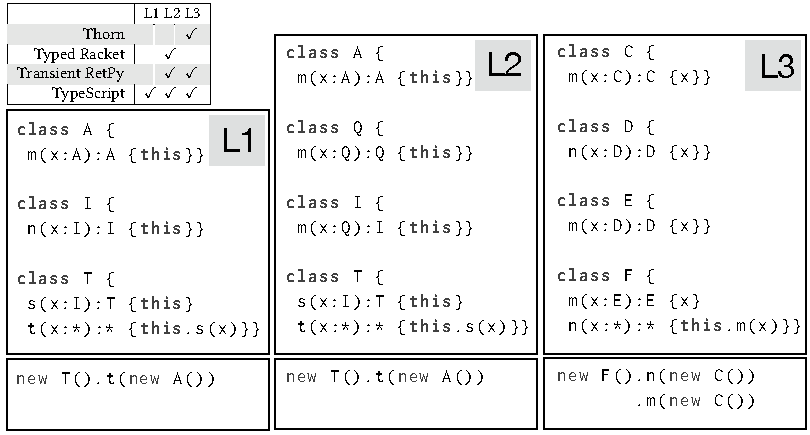
\includegraphics[width=.7\columnwidth]{../figures/litm}
   \caption{Gradual typing semantic litmus tests.}\label{litmus}
\end{wrapfigure}

\noindent In this paper we have compared the essence of four gradual type
system designs, namely TypeScript, Thorn, Typed Racket, and Transient Python.
Our formalization have shown that they differ in which programs are viewed as
statically correct. Thorn distinguishes between concrete and like types,
whereas Transient uses the notion of consistency to determine if values may be
compatible. A perhaps more surprising result is that even at runtime these
languages do not agree on what constitutes a valid program. Consider
\figref{litmus} which shows three small programs -- well-typed in all four
languages. These synthetic examples consist of a class table and a top-level
expression. All three will execute without getting stuck under TypeScript's
permissive semantics.  {\bf L1} fails in all other semantics because \A is not
a subtype of \xt I (Thorn) and \A and \xt I have different sets of methods
(Racket and Python).  {\bf L2} fails in Thorn because the concrete type checks
require subtyping of \A and \xt I to hold. {\bf L3} fails in Thorn because \n
casts an instance of \C to \xt E, despite \C not being a subtype of \xt E.
{\bf L3} also fails in Racket as \xt{F.m} casts an instance of \C to \xt E,
which in turn requires \C.\m to only take and return values of type \D, which
is then called with an instance of a \C. Transient, in contrast, can run {\bf
L3} without error, as, unlike Thorn, it does not compare argument types, and,
unlike Racket, it does not recall the prior cast to \xt E. Thus given these
three programs and the ability to observe errors, one can divine which
semantics a language implements.

Another open question for gradual type system designers is performance of
the resulting implementation. On the one hand, type annotations are a source
of information about programmer intent that could be used to generate
efficient code.  On the other hand, without soundness guarantees this
information cannot be relied upon and becomes, at best, hints that can be
used in heuristic-driven code generation.  The different languages do make
some guarantees which become apparent in our translations -- when the
translation generate static method invocations, for Thorn, Racket and
Python, these invocations can be optimized. The price for these guarantees
comes in the form of casts and wrappers which are not be needed in a fully
dynamic program. The nature of these casts and their dynamic frequency will
make a significant difference to end users.  Thorn inserts them at
boundaries of concrete types only. Racket inserts them whenever a value
crosses either a typed or untyped boundary. Lastly, Transient Python inserts
casts after variable reads. The casts themselves are different, Thorn and
Python merely check for subtyping whereas Racket's casts require allocation.

This paper has introduced \kafka, a framework for comparing the designs of
gradual type systems for object-oriented languages. We have proven \kafka's
type system to be sound in the presence of the dynamic generation of wrapper
classes. Then we have introduced four translations from idealized fragments
of real programming language into \kafka. These translations are shown to
generate well-typed \kafka code. The features that are required to support
gradual types include subtype casts, the ability to generate new classes and
for classes to transparently interpose on target objects. \kafka has proven
to be a versatile vehicle for deconstructing the designs of gradual type
systems.

Going forward there are some issues we wish to investigate further.  We do
not envision that supporting nominal subtyping within \kafka will pose
problems, it would only take adding a nominal cast and changing the
definition of classes. Then nominal and structural could coexist. A more
challenging question is to handle the intricate semantics of Monotonic
Python. For these we would need a somewhat more powerful cast operation.
Rather than building each new cast into the calculus itself, it would be
interesting to axiomatize the correctness requirements for a cast and let
users define their own cast semantics.

\newpage

\bibliographystyle{unsrturl}
\bibliography{../../bib/jv,../../bib/all}

\clearpage

\appendix
%%%%%%%%%%%%%%%%%%%%%%%%%%%%%%%%%%%%%%%%%%%%%%%%%%%%%%%%%%%%%%%%%%%%%%%%%%%%%%
%%%%%%%%%%%%%%%%%%%%%%%%%%%%%%%%%%%%%%%%%%%%%%%%%%%%%%%%%%%%%%%%%%%%%%%%%%%%%%
\section{Full \kafka Definition}%%%%%%%%%%%%%%%%%%%%%%%%%%%%%%%%%%%%
%%%%%%%%%%%%%%%%%%%%%%%%%%%%%%%%%%%%%%%%%%%%%%%%%%%%%%%%%%%%%%%%%%%%%%%%%%%%%%
%%%%%%%%%%%%%%%%%%%%%%%%%%%%%%%%%%%%%%%%%%%%%%%%%%%%%%%%%%%%%%%%%%%%%%%%%%%%%%
\label{appendix:kafka}

\subsection{Well-formedness}

The well-formedness judgments for \kafka are defined for programs, classes, methods, fields, and types.

\vspace{-1cm}

\begin{figure}[!h]
	\small
\begin{minipage}{\textwidth}\begin{tabular}{ll}  
\begin{minipage}{7cm}\begin{mathpar}  
\opdef{~\WFq{\K~\e~\s}}{\text{Well-formed program}}
\vspace{-3mm}
\IRule{WP}{
  \EnvType\emptyset\s\K\e\t \\\\
  \WFtype\K\s \\\\
  \k \in \K \implies \WF{}\cdot\K\k
}{
  \WFq{\K~\e~\s}
}
\end{mathpar}\end{minipage}& \begin{minipage}{5.5cm}\begin{mathpar} 

\opdef{\WF{}\s\K {\Class\C{\fd[1]..}{\md[1]..}}}{\text{Well-formed class}}
\vspace{-2.5mm}
\IRule{WC}{
 \WF {}{}\K {\fd[1]..} \\\\
 \WF {\this:\C~}\s\K {\md[1]..} \\\\
  \cload{\md[1]..~\fd[1]..}
}{
 \WF {}\s\K {\Class \C {\fd[1]..}{\md[1]..}}
}
\end{mathpar}\end{minipage}\end{tabular}\end{minipage}\end{figure}

% \vspace{-1cm}

% The \xt{nodups} function states that there are no overloaded 
% field or method names within the given field and method definitions. \\

\small
\opdef{~\WF \Env\s\K \md}{Well-formed methods}
\vspace{-1mm}
\begin{mathpar}
\IRule[width=18em]{WT1}{
 \Envp = \Env{~\Ftype\x\any} \\
 \EnvType \Envp\s\K\e\any\\
 \WFtype\K\any \\
}{
 \WF \Env\s\K {\Mdef\m\x\any\any\e}
}

% \IRule[width=18em]{WT2}{
\IRule{WT2}{
 \Envp = \Env{~\Ftype\x\C}\\ 
 \EnvType \Envp\s\K\e\Cp\\
 \WFtype\K\C \\
 \WFtype\K\Cp \\
}{
 \WF \Env\s\K {\Mdef\m\x\C\Cp\e}
}
\end{mathpar}

\begin{figure}[!h]
	\small
\begin{minipage}{\textwidth}\begin{tabular}{lll}  
\begin{minipage}[t]{3.7cm}\begin{mathpar}  
\vspace{4mm}
\opdef{~\WFtype \K {\fd}}{\text{Well-formed fields}}
% \vspace{-3mm}
\IRule{WF}{
%  ~\\\\
 \WFtype\K\t 
}{
 \WFtype\K{\Fdef\f\t}
}
\end{mathpar}\end{minipage}& \begin{minipage}[t]{4.2cm}\begin{mathpar} 
 
\opdef{~\WFtype\K\t}{\text{Well-formed types}}
% \vspace{-3mm}
\IRule{WA}{
  ~\\\\
}{
 \WFtype\K\any
}

\IRule{WC}{
 ~\\\\
 \C \in \K
}{
 \WFtype\K\C
}
\end{mathpar}\end{minipage}& \begin{minipage}[t]{5cm}\begin{mathpar} 

\opdef{~\WFtype\K\s}{\text{Well-formed heaps}}
\IRule{WH}{
\Bind\ap{\obj\C{\a[1] ..}}~\in~\s \implies \\\\
\Class\C{\fd[1]..}{\md[1]..}\in\K ~~~\wedge~~~  
\EnvType\cdot\s\K{\a[1]}{\t[1]} ~..
}{
 \WFtype\K\s
}
\end{mathpar}\end{minipage}\end{tabular}\end{minipage}\end{figure}

\subsection{Expression typing}

The expression typing judgments for \kafka includes in ascending order as listed in the formalism:
variable, untyped address, subsumption, field assignment, field read, static method invocation, dynamic method invocation, object creation,
subtype cast, typed address.


\opdef{\EnvType\Env\s\K\e\t}{\e has type \t in environment \Env against heap \s and class table \K}
%\vspace{-2mm}
\begin{mathpar}
\IRule{KT-VAR}{
   ~\\\\
   ~\\\\
   \HasType \Env\x\t
 }{
   \EnvType \Env\s\K\x\t
}

\IRule{KT-SUB}{
  ~\\\\
  \EnvType \Env\s\K\e\tp \\\\
 \StrSub \cdot\K \tp \t
 }{
  \EnvType \Env\s\K\e\t 
}   

\IRule{KT-READ}{
  ~\\\\
  \HasType\Env\this\C \\\\
  \Fdef\f\t \in \App\K\C
}{
  \EnvType \Env\s\K{\FRead\f}\t
}  

\IRule{KT-REFREAD}{
  \s(\a) = \C\{..\} \\\\
  \Fdef\f\t \in \App\K\C
}{
  \EnvType \Env\s\K{\FReadR\a\f}\t
}  

\IRule{KT-WRITE}{
  \HasType\Env\this\C \\\\
  \Fdef\f\t \in \App\K\C \\\\
  \EnvType \Env\s\K\e\t
}{
  \EnvType \Env\s\K{\FWrite\f\e}\t
}    

\IRule[width=12em]{KT-REFWRITE}{
  \s(\a) = \C\{..\} \\\\
  \Fdef\f\t \in \App\K\C \\\\
  \EnvType \Env\s\K\e\t
}{
  \EnvType \Env\s\K{\FWriteR\a\f\e}\t
}  

\IRule[width=16em]{KT-CALL}{
  \EnvType \Env\s\K\e\C \\\\
  \EnvType \Env\s\K\ep\t \\\
  \Mtype\m\t\tp \in \App\K\C 
}{
  \EnvType \Env\s\K{\KCall\e\m\ep\t\tp}\tp
}    

\IRule{KT-DYNCALL}{
  ~\\\\
  \EnvType \Env\s\K\e\any \\\\
  \EnvType \Env\s\K\ep\any
}{
  \EnvType \Env\s\K{\DynCall\e\m\ep}\any
}    

\IRule[width=20em]{KT-NEW}{
  ~\\\\
  \EnvType \Env\s\K{\e[1]}{\t[1]}..\\\\
  \Class \C {\Fdef{\f[1]}{\t[1]}..}{\md[1]..} \in \K
}{
  \EnvType\Env\s\K{\New\C{\e[1]..}}\C
}

\IRule{KT-SUBCAST}{
  \EnvType \Env\s\K\e\tp
}{
  \EnvType \Env\s\K{\SubCast\t\e}\t
}

\IRule{KT-BEHCAST}{
  \EnvType \Env\s\K\e\tp
}{
  \EnvType \Env\s\K{\BehCast\t\e}\t
}

\IRule{KT-REFTYPE}{
  \s(\a) = \obj\C{\ap[1]..}
}{
  \EnvType \Env\s\K\a\C
}

\IRule{KT-REFANY}{
 }{
   \EnvType \Env\s\K\a\any
}
\end{mathpar}

\subsection{Dynamic function}

The \xt{dyn} function returns all the methods with $\star$ type for a particular set of 
signatures of method typing.

\begin{mathpar}
\IRule{DYNE}{
}{
  \dyn{\cdot} = \cdot
}

\IRule{DYN}{
 \dyn{\mt[1]..} = \mtp[1].. \\
}{
  \dyn{\Mtype{\m}{\t}{\t} ~\,\mt[1]..} = \Mtype{\m}{\any}{\any}~\,\mtp[1]..
}
\end{mathpar}

\subsection{Signature function}

The \xt{signature} function returns method typing signatures ($\mt$) of method definitions ($\md$).

\begin{mathpar}
\IRule{SGE}{
}{
  \sign{\cdot} = \cdot
}

\IRule{SG}{
  \md = \Mdef\m\x\t\t\e \\
  \sign{\md[1]..} = \mt[1].. \\
}{
  \sign{\md\,\md[1]..} = \Mtype\m\t\t~~\mt[1]..
}
\end{mathpar}

\subsection{Names function}

The \xt{names} function (\names{\fd[1]..}, \names{\md[1]..}, \names{\mt[1]..}) takes either field definitions, method definitions, or 
method typings, and returns the name of the respective fields or methods.

\subsection{Duplicated method names}

The \xt{nodups} function (\cload{\mt[1]..}, \cload{\md[1]..}) takes either
method definitions or method typings, and ensures there are no duplicates.

\clearpage

\section{Source language syntax and semantics}


\subsection*{Well-formedness for Thorn}

The well-formedness judgments for Thorn is similar to the well-formedness judgments of \kafka with the addition
of well-formed optional types ($\CW$). The turnstile ($\vdash_{\!s}$) of all source language judgment is characterized with s.

\begin{figure}[!h]
	\small
\begin{minipage}{\textwidth}\begin{tabular}{ll}  
\begin{minipage}{7cm}\begin{mathpar}  
\hspace{-1cm}
\opdef{~\WFpW{\e}{\K}}{\text{Well-formed programs}}
\vspace{-3mm}
\IRule{WP}{
  ~\\\\
  \k \in \K \implies \WFW{}\K\k \\
  \EnvTypeW\Env\K\e\t
}{
  \WFpW\e\K
}
\end{mathpar}\end{minipage}& \begin{minipage}{6.0cm}\begin{mathpar}
%\vspace{-6mm}

\opdef{\WFW{}\s\K {\Class\C{\fd[1]..}{\md[1]..}}}{\text{Well-formed classes}}
\vspace{-1mm}
\IRule[width=25em]{WCL}{
 \cload{\fd[1],\md[1]..} \\
 \fd\in\fd[1]..\implies \WFW {}\K \fd \\
 \md\in\md[1]..\implies \WFW {\text{this}:\C~}\K \md 
}{
 \WFW {}\K {\Class \C {\fd[1]..}{\md[1]..}}
}
\end{mathpar}\end{minipage}\end{tabular}\end{minipage}

\vspace{6mm}

\begin{minipage}{\textwidth}\begin{tabular}{l}  
\begin{mathpar}  
\hspace{-7.5cm}                             
\opdef{~\WFW \Env\s\K \md}{\text{Well-formed methods}}

\vspace{-3mm}

\IRule[width=18em]{WT}{
 \EnvTypeW {\Env{~\Ftype\x\C}~}\K\e\D\\
 \WFtypeW\K\C \\
 \WFtypeW\K\D \\
}{
 \WFW \Env\K {\Mdef\m\x\C\D\e}
}

\IRule[width=18em]{WWT}{
 \EnvTypeW {\Env{~\Ftype\x\t}~}\K\e\tp\\
 \WFtypeW\K\t \\
 \WFtypeW\K\tp \\
 \kty\t = \kty\tp = \any
}{
 \WFW \Env\K {\Mdef\m\x\t\tp\e}
}
\end{mathpar}\end{tabular}\end{minipage}

\vspace{4mm}

\begin{minipage}{\textwidth}\begin{tabular}{ll}  
\begin{minipage}{7cm}\begin{mathpar}  
% \hspace{-1cm}
\opdef{~\WFtypeW \K {\Fdef\f\t}}{\text{Well-formed fields}}
\vspace{-3mm}
\IRule{WF}{
 \WFtypeW\K\t 
}{
 \WFtypeW\K{\Fdef\f\t}
}

\end{mathpar}\end{minipage}& \begin{minipage}{6.0cm}\begin{mathpar} 
\hspace{-2cm}
\opdef{~\WFtypeW\K\t}{\text{Well-formed types}}
\vspace{-3mm}

\IRule{WA}{
}{
 \WFtypeW\K\any
}

\IRule{WC}{
 \C \in \K
}{
 \WFtypeW\K\C
}

\IRule{WW}{
 \C \in \K
}{
 \WFtypeW\K{\CW}
}
\end{mathpar}\end{minipage}\end{tabular}\end{minipage}
\end{figure}

% \clearpage

\subsection*{Well-formedness for Typed Racket, TypeScript, Transient}

The well-formedness judgments for Typed Racket, TypeScript, and Transient is a subset of the well-formedness judgment for \kafka.

\begin{figure}[!h]
% \vspace{-8mm}
\begin{minipage}{\textwidth}\begin{tabular}{ll}  
\begin{minipage}{4cm}\begin{mathpar} 
\opdef{~$\WFpx{\e}{\K}$}{\text{Well-formed programs}}
\vspace{-2mm}
\IRule{SWF-PROG}{
  \EnvTypex\Env\cdot\K\e\t \\\\
  \k \in \K \implies \WFx{}\cdot\K\k
}{
  \WFpW\e\K
}
\end{mathpar}\end{minipage}& \begin{minipage}{12.0cm}\begin{mathpar} 

\opdef{\WFx{}\s\K {\Class\C{\fd[1]..}{\md[1]..}}}{\text{Well-formed classes}}
\vspace{-3mm}
\IRule[width=25em]{SWF-CLASS}{
 \cload{\fd[1]..,\md[1]..} \\
 \fd\in\fd[1]..\implies \WFx {}{}\K \fd \\
 \md\in\md[1]..\implies \WFx {\this:\C~}{}\K \md 
}{
 \WFx {}{}\K {\Class \C {\fd[1]..}{\md[1]..}}
}
\end{mathpar}\end{minipage}\end{tabular}\end{minipage}
\end{figure}

\opdef{~\WFx \Env{}\K \md}{Well-formed methods}
\begin{mathpar}
\hspace{-8mm}

\IRule[width=18em]{SWF-TYMETH}{
 \EnvTypex {\Env{~\Ftype\x\C}~}\K\e\D\\
 \WFtypex\K\C \\
 \WFtypex\K\D \\
}{
 \WFx \Env{}\K {\Mdef\m\x\C\D\e}
}

\IRule[width=18em]{SWF-DYMETH}{
 \EnvTypex {\Env{~\Ftype\x\any}~}\K\e\any\\
 \WFtypex\K\any \\
 \WFtypex\K\any
}{
 \WFx \Env{}\K {\Mdef\m\x\any\any\e}
}
\end{mathpar}


\begin{figure}[!h]
% \vspace{-8mm}
\begin{minipage}{\textwidth}\begin{tabular}{ll}  
\begin{minipage}{4cm}\begin{mathpar} 
\opdef{~\WFtypex \K {\Fdef\f\t}}{\text{Well-formed fields}}
% \vspace{-3mm}
\IRule{SWF-FIELD}{
 \WFtypex\K\t 
}{
 \WFtypex\K{\Fdef\f\t}
}
\end{mathpar}\end{minipage}& \begin{minipage}{10.0cm}\begin{mathpar} 

\hspace{-5cm}

\opdef{~\WFtypex\K\t}{\text{Well-formed types}}
% \vspace{-3mm}
\IRule{SWT-ANY}{
}{
 \WFtypex\K\any
}

\IRule{SWT-TYPE}{
 \C \in \K
}{
 \WFtypex\K\C
} 
\end{mathpar}\end{minipage}\end{tabular}\end{minipage}
\end{figure}

\clearpage

\section{Litmus tests in source language}

\subsection*{Thorn}

Below we present the three litmus tests, presented in \figref{litmus}, in Thorn syntax. \\

\noindent
\textbf{Litmus Test 1}:
\begin{lstlisting}
class A() {
   def m(x:A):A = this;}

class I() {
   def n(x:I):I = this;}

class T() {
   def s(x:I):T = this;
   def t(x:dyn):dyn = this.s(x);}

 T().t(A());
\end{lstlisting}

\noindent
\textbf{Litmus Test 2}:
\begin{lstlisting}
class Q() {
   def n(x: Q): Q = this;}

class A() {
   def m(x:A): A = this;}

class I() {
   def m(x:Q):I = this;}

class T() {
   def s(x:I):T = this; 
   def t(x:dyn):dyn = this.s(x);}
   
 T().t(A());   
\end{lstlisting}


\noindent
\textbf{Litmus Test 3}:
\begin{lstlisting}
class C() { 
   def m(x:C):C = x;}

class D() {
   def n(x:D):D = x;}
      
class E() {
   def m(x:D):D = x;}      

class F() {
   def m(x:E):E = x;
   def n(x:dyn):dyn = this.m(x);} 
	     
  F().n(C()).m(C());
\end{lstlisting}
% 
% \begin{figure}[!t]
% \small
% \begin{tabular}{@{}cc}
%   \begin{tabular}{|@{}cc@{\hspace{1mm}}|}\hline
%   \begin{minipage}{4.6cm}
%     \begin{lstlisting}
% class A() {
%  def m(x:A):A = this;}
% 
% class I() {
%  def n(x:I):I = this;}
% 
% class T() {
%  def s(x:I):T = this;
%  def t(x:dyn):dyn = 
%              this.s(x);}
%       \end{lstlisting}    
%   \end{minipage}
% &
%   \begin{minipage}{4.6cm}
%     \begin{lstlisting}
% class A() {
%  def m(x:A): A = this;}
% 
% class I() {
%  def m(x:Q):I = this;}
% 
% class T() {
%  def s(x:I):T = this; 
%  def t(x:dyn):dyn = 
%              this.s(x);}
%       \end{lstlisting}    
%   \end{minipage}
% \\[2mm]
% (Litmus test 1) & (Litmus test 2)\\[3mm]
%   \begin{minipage}{4.3cm}
%     \begin{lstlisting}
% class C() { 
%   def m(x:C):C = x;}
% 
% class D() {
%   def n(x:D):D = x;}
%       
% class E() {
%   def m(x:D):D = x;}      
% 
% class F() {
%   def m(x:E):E = x;
%   def n(x:dyn):dyn =
% 	     this.m(x);}       
%       \end{lstlisting}    
%   \end{minipage}
% &
% \begin{minipage}{4cm}
% \begin{tabular}{|@{}c@{\hspace{1mm}}|}\hline
%   \begin{minipage}{4cm}
%     \begin{lstlisting}
% class Q() { 
%   def n(x:C):C = 
% 	             this;}
%     \end{lstlisting}    
%   \end{minipage}
%  \\
%   (Auxiliary classes)\\\hline
% \end{tabular}
% \\ \\ \\  
% \begin{tabular}{|@{}c@{\hspace{1mm}}|}\hline
%   \begin{minipage}{4cm}
%     \begin{lstlisting}
%   T().t(A());
%     \end{lstlisting}    
%   \end{minipage}
%   \\
%   (Program 1-2)\\\hline
% \end{tabular}
% \\ \\ \\  
% \begin{tabular}{|@{}c@{\hspace{1mm}}|}\hline
%   \begin{minipage}{4cm}
%     \begin{lstlisting}
%    F().n(C()).m(C());
%     \end{lstlisting}    
%   \end{minipage}
%   \\
%   (Program 3)\\\hline
% \end{tabular}
% \end{minipage}
% \\[2mm]
% (Litmus test 3) &
% \\\hline
%   \end{tabular}
% 
% \end{tabular}
% \end{figure}


\subsection*{TypeScript}

Below we present the three litmus tests, presented in \figref{litmus}, in TypeScript syntax. \\

\noindent
\textbf{Litmus Test 1}:
\begin{lstlisting}
class A {
    m(x: A): A { return this }
}

class I {
    n(x:I):I { return this }
}

class T {
    s(x: I): T { return this }
    t(x: any): any { return this.s(x) }
}

new T().t(new A())
\end{lstlisting}

\noindent
\textbf{Litmus Test 2}:
\begin{lstlisting}
class Q {
    n(x: Q): Q { return this }
}

class A {
    m(x: A): A { return this }
}

class I {
    m(x:Q):I { return this }
}

class T {
    s(x: I): T { return this }
    t(x: any): any { return this.s(x) }
}

new T().t(new A())
\end{lstlisting}


\noindent
\textbf{Litmus Test 3}:
\begin{lstlisting}
class C {
    m(x: C): C { return x }
}

class D {
    n(x: D): D { return x }
}

class E {
    m(x: D): D { return x }
}

class F {
    m(x: E): E { return x }
    n(x: any): any { return this.m(x) }
}

new F().n(new C()).m(new C())
\end{lstlisting}




\subsection*{Typed Racket}

Below we present the three litmus tests, presented in \figref{litmus}, in Typed Racket syntax. \\

\noindent
\textbf{Litmus Test 1}:

\begin{lstlisting}
#lang racket

(module u racket
  (define Tp% (class object%
                (super-new)
                (define/public (t x) (send this s x))))
  (provide Tp%))

(module t typed/racket
  (require/typed (submod ".." u) [Tp% (Class [t (-> Any Any)])])
  (define-type A (Instance (Class (m (-> A A)))))
  (define-type I (Instance (Class (n (-> I I)))))
  (define-type T (Instance (Class (s (-> I T)))))
  (define T% (class Tp%
               (super-new)
               (: s (-> I T))
               (define/public (s x) this)))
  (define A% (class object%
               (super-new)
               (: m (-> A A))
               (define/public (m x) this)))
  (provide T% A%))

(require 't)
(send (new T%) t (new A%))
\end{lstlisting}

\noindent
\textbf{Litmus Test 2}:

\begin{lstlisting}
#lang racket

(module u racket
  (define Tp% (class object%
                (super-new)
                (define/public (t x) (send this s x))))
  (provide Tp%))

(module t typed/racket
  (require/typed (submod ".." u) [Tp% (Class [t (-> Any Any)])])
  (define-type Q (Instance (Class (n (-> Q Q)))))
  (define-type A (Instance (Class (m (-> A A)))))
  (define-type I (Instance (Class (m (-> Q I)))))
  (define-type T (Instance (Class (s (-> I T)))))
  (define T% (class Tp%
               (super-new)
               (: s (-> I T))
               (define/public (s x) this)))
  (define A% (class object%
               (super-new)
               (: m (-> A A))
               (define/public (m x) this)))
  (provide T% A%))

(require 't)
(send (new T%) t (new A%))
\end{lstlisting}

\noindent\textbf{Litmus Test 3}:

\begin{lstlisting}
#lang racket

(module u racket
  (define Fp% (class object%
                (super-new)
                (define/public (n x) (send this m x))))
  (provide Fp%))

(module t typed/racket
  (require/typed (submod ".." u) [Fp% (Class [n (-> Any Any)])])
  (define-type C (Instance (Class (m (-> C C)))))
  (define-type E (Instance (Class (m (-> D D)))))
  (define-type D (Instance (Class (n (-> D D)))))
  (define F% (class Fp%
               (super-new)
               (: m (-> E E))
               (define/public (m x) x)))
  (define C% (class object%
               (super-new)
               (: n (-> C C))
               (define/public (n x) x)))
  (provide F% C%))

(require 't)
(send (send (new F%) n (new C%)) m (new C%))
\end{lstlisting}


\subsection*{Transient}

Below we present the three litmus tests, presented in \figref{litmus}, in Reticulated Python (transient) syntax. \\

\noindent
\textbf{Litmus Test 1}:
\begin{lstlisting}
class A:
   def m(self, x:A) -> A:
    return self
    
class I:
   def n(self, x:I) -> I:
     return self

class T:
   def s(self, x:I) -> T:
     return self
   def t(self, x:Dyn) -> Dyn:
     return self.s(x)

 T().t(A())
\end{lstlisting}

\noindent
\textbf{Litmus Test 2}:
\begin{lstlisting}
class C:
   def n(self, x:C) -> C:
     return self

class Q:
   def m(self, x:Q) -> Q:
     return self     
     
class A:
   def m(self, x:A) -> A:
     return self

class I:
   def m(self, x:Q) -> I:
     return self

class T:
   def s(self, x:I) -> T:
     return self
   def t(self, x:Dyn) -> Dyn:
     return self.s(x)

 T().t(A())
\end{lstlisting}


\noindent
\textbf{Litmus Test 3}:
\begin{lstlisting}
class C:
  def m(self, x:C) -> C:
     return x
     
class D:
  def n(self, x:D) -> D:
     return x
     
class E:
  def m(self, x:D) -> D:
     return x
     
class F:
  def m(self, x:E) -> E:
     return x   
  def n(self, x:Dyn) -> Dyn:
     return self.m(x)

 F().n(C()).m(C())
\end{lstlisting}

% 
% \begin{figure}[!t]
% \small
% \begin{tabular}{@{}cc}
%   \begin{tabular}{|@{}cc@{\hspace{1mm}}|}\hline
%   \begin{minipage}{4.6cm}
%     \begin{lstlisting}
% class A:
%   def m(self, x:A) -> A:
%     return self
%     
% class I:
%   def n(self, x:I) -> I:
%     return self
% 
% class T:
%   def s(self, x:I) -> T:
%     return self
%   def t(self, x:Dyn) -> Dyn:
%     return self.s(x)
% \end{lstlisting}    
%   \end{minipage}
% &
%   \begin{minipage}{4.6cm}
%     \begin{lstlisting}
% class C:
%   def n(self, x:C) -> C:
%     return self
% class A:
%   def m(self, x:A) -> A:
%     return self
% class I:
%   def m(self, x:Q) -> I:
%     return self
% class T:
%   def s(self, x:I) -> T:
%     return self
%   def t(self, x:Dyn) -> Dyn:
%     return self.s(x)
%       \end{lstlisting}    
%   \end{minipage}
% \\[2mm]
% (Litmus test 1) & (Litmus test 2)\\[3mm]
%   \begin{minipage}{4.6cm}
%     \begin{lstlisting}
% class C:
%  def m(self, x:C) -> C:
%     return x
% class D:
%  def n(self, x:D) -> D:
%     return x   
% class E:
%  def m(self, x:D) -> D:
%     return x    
% class F:
%  def __init__(self, f):
%     self.f = f
%  def m(self, x:E) -> E:
%     return x   
%  def n(self, x:Dyn) -> Dyn:
%     return self.m(x)
%    \end{lstlisting}    
%   \end{minipage}
% &
%   \begin{minipage}{4.6cm}
% \begin{minipage}{4.4cm}
% \begin{tabular}{|@{}c@{\hspace{1mm}}|}\hline
%   \begin{minipage}{4cm}
%     \begin{lstlisting}
% class Q:
%  def n(self, x:Q) -> Q:
%    return self
%     \end{lstlisting}    
%   \end{minipage}
%  \\
%   (Auxiliary classes)\\\hline
% \end{tabular}
% \\ \\ \\  
% \begin{tabular}{|@{}c@{\hspace{1mm}}|}\hline
%   \begin{minipage}{4.4cm}
%     \begin{lstlisting}
%  T().t(A())
%    \end{lstlisting}    
%   \end{minipage}
%   \\
%   (Program 1-2)\\\hline
% \end{tabular}
% \\ \\ \\  
% \begin{tabular}{|@{}c@{\hspace{1mm}}|}\hline
%   \begin{minipage}{4.4cm}
%     \begin{lstlisting}
%    F().n(C()).m(C());
%     \end{lstlisting}    
%   \end{minipage}
%   \\
%   (Program 3)\\\hline
% \end{tabular}
% \end{minipage} 
%   \end{minipage}
% \\[2mm]
%  (Litmus test 3) &  \\\hline
%   \end{tabular}
%   &
% 
% \end{tabular}
% \end{figure}

\clearpage

% \subsection*{Transient expression typing}
% 
% \opdef{\ConvertE\K{tr}\t\tp}{type convertibility between \t and \tp.}
% \begin{mathpar}
% \IRule{STTC-SUB}{
%   \ConSub\cdot\K\t\tp
% }{
%   \ConvertE\K{tr}\t\tp
% }
% 
% \IRule{STTC-TOANY}{
% }{
%   \ConvertE\K{tr}\t\any
% }
% 
% \IRule{STTC-ANYCONC}{
% }{
%   \ConvertE\K{tr}\any\tp
% }
% \end{mathpar} \\
% 
% \opdef{\EnvTypeT\Env\K\e\t}{\e has type \t in environment \Env against heap  and class table \K}
% \begin{mathpar}
% \IRule{STT-VAR}{
%    ~\\\\
%    ~\\\\
%    ~\\\\
%    \HasType \Env\x\t
%  }{
%    \EnvTypeT \Env\K\x\t
% }
% 
% \IRule{STT-GET}{
%    ~\\\\
%    ~\\\\   
%    \HasType \Env\this\C \\\\
%   \Fdef\f\t \in \App\K\C
% }{
%   \EnvTypeT \Env\K{\FRead\f}\t
% }    
% 
% \IRule[width=20em]{STT-SET}{
%   \HasType \Env\this\C \\\\
%   \Fdef\f\t \in \App\K\C \\\\
%   \EnvTypeT \Env\K\e\tp \\\\
%   \ConvertE\K{tr}\tp\t
% }{
%   \EnvTypeT \Env\K{\FWrite\f\e}\t
% }    
% 
% \IRule[width=20em]{STT-CALL}{
%   \EnvTypeT \Env\K\e\C \\\\
%   \EnvTypeT \Env\K\ep\tpp \\\\
%   \ConvertE\K{tr}\tpp\any \\\\
%   \Mtype \m\t\tp\in \App\K\C
% }{
%   \EnvTypeT \Env\K{\Call\e\m\ep}\tp
% }    
% 
% \IRule[width=20em]{STT-DCALL}{
%   \EnvTypeT \Env\K\e\any \\\\
%   \EnvTypeT \Env\K\ep\tpp \\\\
%   \ConvertE\K{tr}\tpp\any
% }{
%   \EnvTypeT \Env\K{\Call\e\m\ep}\any
% }    
% 
% \IRule{STT-NEW}{
%  \EnvTypeT \Env\K{\e[1]}{\tp[1]}..\\\\
%  \ConvertE\K{tr}{\tp[1]}{\t[1]}.. \\\\
%  \Class \C {\fd[1]..}{\md[1]..} \in \K
% }{
%   \EnvTypeT \Env\K{\New\C{\e[1]..}}\C
% }
% \end{mathpar}


% \clearpage

% \section{Translations}
% \renewcommand{\trulename}[1]{#1}
% 
% \subsection{Thorn}
% 
% \begin{figure}[!h]
% \begin{tabular}{@{}l@{~ ~ ~ ~~~~~~~~~~~~~~~~~~~~~~~~~~~~~~~~~~~~}ll}
% \small
%   \hspace{-.5cm}\begin{minipage}{8cm}  
% \begin{tabbing}
% \TR{\Class \C{\fd[1]..}{\md[1] .. }}\= = \src{ \Class \C{ \fdp[1]..}{\mdp[1]..~ \mdpp[1]..}} 
% \HS \WHERE~\= \fdp[1] = \src{\Ftype\f{\kty\t}} .., \HS\HS\HS\HS\HS \=\fd[1] = \Ftype\f\t ..   \\
% \> \mdp[1] = \src{\Mdef\m\x{\kty{\t[1]}}{\kty{\t[2]}}{\ep}} .., \HS \> \md[1] = \Mdef\m\x{\t[1]}{\t[2]}\e ..,\HS\HS\> \ep = \TAG{\e}{\this:\C\,\x:{\t[1]}}{\t[2]} ..,\\
% \> \mdpp[1] = \src{\Mdef\m\x\any\any{\SubCast\any{\KCall\this\m{\SubCast{\t[1]}\x}{\t[1]}{\t[2]}}}}
% \HS \IF \kty{\t[1]} = \D \OR \kty{\t[2]} = \D\\
%           \>\hspace{1cm} empty \HS  {\bf otherwise}  ..   \\
% \TR{\k .. \e} \>= \TR{\k} .. \TRG{\e}\cdot \\
% \TR{\x:\t~\Env} \>= \x : \kty{\t} ~ \TR\Env
% \end{tabbing}
% \begin{tabbing}
% \trulename{TTH1} \TRG{\x}\Env \hspace{1.4cm}\= = \src \x
% \\[1mm]       
% \trulename{TTH2} \TRG{\FRead\f}\Env \> = \src{\FRead\f} 
% \\[1mm]
% \trulename{TTH3} \TRG{\FWrite\f\e}\Env \> = \src{\FWrite\f\ep} \hspace{.5cm} \=
% \WHERE\HS\= \TypeCk{\K, \Env}\this\C, \HS  \Ftype\f\t\In\App\K\C, \HS \ep = \TAG\e\Env{\kty\t}
% \\[1mm]
% \trulename{TTH4} \TRG{\Call{\e[1]}\m{\e[2]}}\Env \>= \src{\DynCall{\ep[1]}{\m}{\ep[2]}} 
% \HS  \>\WHERE\HS \TypeCk{\K,\Env}{\e[1]}\t, \HS \kty\t=\any, \HS
%  \ep[1]= \TRG{\e[1]}\Env, \HS \ep[2]=\TAG{\e[2]}\Env\any
% \\[1mm]
% \trulename{TTH5} \TRG{\Call{\e[1]}\m{\e[2]}}\Env \>= \src{\KCall{\ep[1]}{\m}{\ep[2]}{\t[2]}{\tp[2]}} 
% \>\WHERE\HS   \TypeCk{\K,\Env}{\e[1]}\C, \HS  \ep[1] = \TRG{\e[1]}\Env, \HS
%  \Mtype\m{\t[1]}{\tp[1]}\In\App\K\C, \HS  \ep[2] = \TAG{\e[2]}\Env{\t[2]}, \\
%  \> \> \> \t[2] = \kty{\t[1]}, \HS \tp[2] = \kty{\tp[1]}
% \\[1mm]
% \trulename{TTH6} \TRG{\New\C{\e[1]..}}\Env\> = \src{\New\C{\ep[1]..}} 
%      \>\WHERE\HS    \Ftype{\f[1]}{\t[1]}\In\C, \HS  \ep[1] = \TAG{\e[1]}\Env{\t[1]} ..
% \\[1mm]
% \trulename{TTH7} \TAG\e\Env\t\> = \src\ep \> \WHERE\HS  \EM{\K\vdash\kty\tp \Sub \kty\t}, \TypeCk{\K,\Env}\e\tp, \ep = \TRG\e\Env
% \\[1mm]
% \trulename{TTH8} \TAG\e\Env\t \>= \src{\SubCast{\kty\t}\ep}
% \>\WHERE\HS  \EM{\K\vdash\kty\tp \not\Sub \kty\t}, \TypeCk{\K,\Env}\e\tp, \ep = \TRG\e\Env
% \end{tabbing}
% \end{minipage}
% \end{tabular}
% \caption{Thorn}
% \end{figure}
% 
% \subsection{TypeScript}
% 
% \begin{figure}[!h]
% \begin{tabular}{@{}l@{~ ~ ~ ~~~~~~~~~~~~~~~~~~~~~~~~~~~~~~~~~~~~}ll}
% \small
%  \hspace{-.5cm}\begin{minipage}{8cm}  
% \begin{tabbing}
% \TR{\Class \C{\fd[1]..}{\md[1] .. } } = \src{ \Class \C{ \fdp[1]..}{\mdp[1]..}}\HS \WHERE\HS
%   \=\fd[1] = \Ftype\f\t ..,\HS\HS\=\fdp[1] = \src{\Ftype\f\any} .., \HS\HS\=\md[1] = \Mdef\m\x{\t[1]}{\t[2]}\e \\
%   \>\mdp[1] = \src{\Mdef\m\x\any\any\ep},\HS\HS \>\>\ep = \TR{\e}
% \end{tabbing}
% \begin{tabbing}
% \trulename{TTS1} \TR{\FRead\f}\HS\HS\HS\HS\= = \src{\FRead\f}
% \\[1mm]
% \trulename{TTS2} \TR{\FWrite\f\e} \> = \src{\FWrite\f\ep} \HS\HS\HS\HS\HS\=\WHERE~\ep=\TR\e
% \\[1mm]
% \trulename{TTS3} \TR\this           \>= \src{\SubCast\any\this}
% \\[1mm]
% \trulename{TTS4} \TR\x \> = \src \x
% \\[1mm]       
% \trulename{TTS5} \TR{\Call{\e[1]}\m{\e[2]}} \> = \src{\DynCall{\ep[1]}{\m}{\ep[2]}} \HS\>\WHERE\HS\ep[1] = \TR{ \e[1]}, \HS \ep[2] = \TR{\e[2]}
% \\[1mm]
% \trulename{TTS6} \TR{\New\C{\e[1]..}} \> = \src{\SubCast\any{\New\C{\ep[1]..}}} \HS \>\WHERE \HS   \ep[1] = \TR{\e[1]} ..
% \end{tabbing}
% \end{minipage}
% \end{tabular}
% \caption{TypeScript}
% \end{figure}
% 
% 
%  \clearpage
% 
% \subsection{Typed Racket}
% 
% \begin{figure}[!h]
% \begin{tabular}{@{}l@{~ ~ ~ ~~~~~~~~~~~~~~~~~~~~~~~~~~~~~~~~~~~~}ll}
%  \small
% \begin{minipage}{8cm}  
% \begin{tabbing}
% \TR{\Class\C{\fd[1]..}{\md[1].. }} =  \src{\Class \C {\fd[1] ..}{\mdp[1].. } }\\
% \hspace{.7cm} \WHERE\HS 
% \mdp[1] = \src{\Mdef\m\x\t\tp{\ep[1]}} ..,\HS\HS
% \md[1] = \Mdef\m\x\t\tp{\e[1]} ..,\HS\HS
% \ep[1] = \TRG{\e[1]}{\x:\t\,\this:\C}
% \end{tabbing}
% \begin{tabbing}
% \trulename{TTK1} \TRG\x\Env = \src{\x}
% \\[1mm]
% \trulename{TTK2} \TRG{\FRead\f}\Env  = \src{\FRead\f}
% \\[1mm]
% \trulename{TTK3} \TRG{\FWrite\f\e}\Env =  \src{\FWrite\f\ep} \hspace{.8cm}
% \=\WHERE
% \= \TypeCk\K{\this}\C, \HS\HS
% \= \Ftype\f\t\In\App\K\C, \hspace{1cm}
% \= \ep = \TAG\e\Env\t
% \\[1mm]
% \trulename{TTK4} \TRG{\Call{\e1[1]}\m{\e[2]}}\Env = \src{\DynCall{\ep[1]}\m{\ep[2]}}\hspace{.8cm}
% \>\WHERE \> \TypeCk{\K,\Env}{\e[1]}\any, \HS
% \> \ep[1] = \TRG{\e[1]}\Env,\HS \hspace{1cm}
% \= \ep[2] = \TAG{\e[2]}\Env\any
% \\
% \trulename{TTK5} \TRG{\Call{\e1[1]}\m{\e[2]}}\Env = \src{\KCall{\ep[1]}{\m}{\ep[2]}{\D[1]}{\D[2]}}\hspace{.8cm}
% \>\WHERE \> \TypeCk{\K,\Env}{\e[1]}\C, \HS
% \> \Mtype\m{\D[1]}{\D[2]}\In\App\K\C, \HS
% \> \ep[1] = \TRG{\e[1]}\Env,\HS 
% \= \ep[2] = \TAG{\e[2]}\Env{\D[1]}
% \\[1mm]
% \trulename{TTK6} \TRG{\New\C{\e[1]..}}\Env =  \src{\New\C{\ep[1]..}}
%    \>\WHERE \> \Ftype{\f[1]}{\t[1]}\In\App\K\C ~..
%    \>       \>  \ep[1] = \TAG{\e[1]}\Env{\t[1]} ~..
% \\[1mm]
% \trulename{TTK7} \TAG\e\Env\t = \src\ep
% \> \WHERE\> \TypeCk{\K,\Env}\e\tp, \HS
% \> \EM{\K\vdash \t \Sub \tp},
% \>  \ep = \TRG\e\Env
% \\[1mm]
% \trulename{TTK8} \TAG\e\Env\t = \src{\BehCast\t\e}
% \>\WHERE\> \TypeCk{\K,\Env}\e\tp, \HS
%    \> \EM{\K\vdash \t \not \Sub \tp}
%    \>     \ep = \TRG\e\Env
% \end{tabbing}
% \end{minipage}
% \end{tabular}
% \caption{Typed Racket}\end{figure}
% 
% 
% \subsection{Transient}
% 
% \begin{figure}[!h]
% \begin{tabular}{@{}l@{~ ~ ~}ll}
%  \small
% \begin{minipage}{8cm}  
% \begin{tabbing}
% \TR{\Class\C{\fd[1]..}{\md[1].. }} =  \src{\Class \C {\fdp[1]..}{\mdp[1].. } }\\
% \hspace{.5cm}  \WHERE\HS \=
%   \fdp[1] = \src{\Ftype\f\any} .., \HS
%   \fd[1] = \Ftype\f\t ..,\HS\HS
%   \mdp[1] = \src{\Mdef\m\x\any\any{\SubCast\t\x ~; ~\ep[1]}} .., \HS
%   \md[1] = \Mdef\m\x\t\tp\e ..,\HS\HS
%    \ep[1] = \TAG\e{\x:\t\,\this:\C}\tp~ ..
% \end{tabbing}
% \begin{tabbing}
% \trulename{TTR1} \TRG\this\Env \hspace{1cm} \= = \src\this
% \\[1mm]
% \trulename{TTR2} \TRG\x\Env \>= \src{\SubCast\t\x} \hspace{1.5cm} \=\WHERE \HS \TypeCk{\K,\Env}\x\t
% \\[1mm]
% \trulename{TTR3} \TRG{\FRead\f}\Env \>= \src{\SubCast\t{\FRead\f}} \>\WHERE\HS  \TypeCk{\K,\Env}\this\C,\HS\HS\=\Ftype\f\t\In\App\K\C
% \\[1mm]
% \trulename{TTR4} \TRG{\FWrite\f\e}\Env \>=  \src{\SubCast\t{\FWrite\f\ep}}
%   \>\WHERE\HS
%   \TypeCk\K\this\C,
%   \> \Ftype\f\t\In\App\K\C, \hspace{.7cm}
%   \= \ep = \TAG\e\Env\any
% \\[1mm]
% \trulename{TTR5}   \TRG{\Call{\e[1]}\m{\e[2]}}\Env \>= \src{\DynCall{\ep[1]}\m{\ep[2]}}
%   \>\WHERE \HS 
%   \TypeCk{\K,\Env}{\e[1]}\any, \HS
%   \> \ep[1] = \TRG{\e[1]}\Env, 
%   \> \ep[2] = \TAG{\e[2]}\Env\any
% \\[1mm]
% \trulename{TTR6} \TRG{\Call{\e[1]}\m{\e[2]}}\Env \>= \src{\SubCast\tp{\KCall{\ep[1]}\m{\ep[2]}\any\any}}
%    \>\WHERE\HS
%    \TypeCk{\K,\Env}{\e[1]}\C,
%    \> \Mtype\m\t\tp\In\App\K\C,\HS
%    \> \ep[1] = \TRG{\e[1]}\Env, \HS\HS
%    \ep[2] = \TAG{\e[2]}\Env\any
% \\[1mm]
% \trulename{TTR7} \TRG{\New\C{\e[1]..}}\Env \>=  \src{\New\C{\ep[1]..}} \>\WHERE\HS
% \Ftype{\f[1]}{\t[1]}\In\App\K\C,
%   \>\ep[1] = \TAG{\e[1]}\Env{\any} ~..
% \\[1mm]
% \trulename{TTR8} \TAG\e\Env\t \>= \src{\SubCast\t\e}
%     \>\WHERE\HS \TypeCk{\K,\Env}\e\tp, \> (\t = \any \OR \tp = \any),\HS \> \ep = \TRG\e\Env
% \\[1mm]
% \trulename{TTR9} \TAG\e\Env\t \>= \src\ep \>\WHERE\HS  \TypeCk{\K,\Env}\e\tp, \HS\>(\EM{\ConSub{}\K\t\tp}),\HS \> \ep = \TRG\e\Env
% \end{tabbing}
% \end{minipage}
% \end{tabular}
% \caption{Transient}\end{figure}
% 
% \clearpage

\section{Proofs of Related Theorems}

In this section, we present the proof of type soundness for the type system of \kafka. The \kafka language includes the behavioural cast
semantics shown in \figref{behavetext}. \\

% \subsection*{}
% 
% Given that $\WFp\K{\e~\s}$ and $\EnvType\cdot\s\K\e\t$, then either there is some $\ep$ and $\Kpp$ (with $\Kp = \K~\Kpp$) 
% such that $\Reduce \K\e\s \Kp\ep\sp$ and $\WFp\Kp{\ep~\sp}$ and $\EnvType\cdot\sp\Kp\ep\t$ hold, 
% or $\e$ is stuck in one of the following forms:
% \begin{itemize} 
% \item $\a$
% \item $\EE[\DynCall\a\m{\ap}]$
% \item $\EE[\SubCast\tp\a]$
% \item $\EE[\BehCast\tp\a]$
% \end{itemize}


\begin{theorem}{Type Soundness of Core \kafka Typing}{}
  
  \begin{conds}
   \cond{\WFq{\K~\e~\s}}\lbl{cond1}
   \cond{$\EnvType\cdot\s\K\e\t$}\lbl{cond3a}
  \end{conds}
  
  \then\axiom{$\Reduce \K\e\s \Kp\ep\sp$}
  \axiom{$\WFp\Kp{\ep~\sp}$}
  \axiom{$\EnvType\cdot\sp\Kp\ep\t$}
  \tor\axiom{$\e$ = $\a$}
  \tor\axiom{$\e$ = $\EE[\DynCall\a\m{\ap}]$}
  \tor\axiom{$\e$ = $\EE[\SubCast\tp\a]$}
  \tor\axiom{$\e$ = $\EE[\BehCast\tp\a]$}  

%   \begin{proof} 
% %   \indana{\trf{cond1}}
% 
%   \end{proof}
\end{theorem}

% We proceed with structural induction on the judgement used to conclude $\EnvType\Env\s\K\e\t$. 
% Note that we refer to rule preconditions from left to right.

% \begin{itemize}
%   \item \RuleRef{KT-VAR}
%         Not applicable, since $\Gamma = \cdot$ and therefore contains no variables.
%   \item \RuleRef{KT-SUB}
%         We apply the IH to the first precondition. If we get stuck in the IH, then the entire
%         expression gets stuck or terminates, trivially. Therefore, the interesting case is when
%         $\Reduce \K\e\s \Kp\ep\sp$, $\WFp\Kp{\ep~\sp}$ and $\EnvType\cdot\sp\Kp\ep\tp$. Since, by the
%         second precondition, we know that $\StrSub \M\K \tp \t$, it follows by weakening of subtyping $\StrSub\M\Kp\tp\t$.
%         We can then apply \RuleRef{W2} to find that $\EnvType\cdot\sp\Kp\ep\t$, and therefore $\Reduce\K\e\s\Kp\ep\sp$, $\WFp\Kp{\ep~\sp}$, and $\EnvType\cdot\sp\Kp\ep\t$, and the theorem holds.
%   \item \RuleRef{KT-READ}
%         Since $\Gamma = \cdot$ by assumption, \RuleRef{KT-READ} cannot have applied.
%   \item \RuleRef{KT-REFREAD}
%         By inversion of $\RuleRef{KT-REFREAD}$, we know that the expression is of form $\FReadR\a\f$. It follows from $\Fdef\f\t \in \App\K\C$ that $\Class\C{\fd[i].. \Fdef\f\t ~ \fd[j] ..}{\md..}$ and from well-formedness of heaps that $\App\sigma\a = \Map\s{\Bind{\a}{\obj\C{\a[i].. ~\ap~ \a[j]..}}}$ that $\EnvType\cdot\s\K\ap\t$. Therefore, $\Reduce\K{\FReadR\a\f}\s\K\ap\s$ and $\WFp\K{\ap~\s}$, so the theorem holds.
%   \item \RuleRef{KT-WRITE}
%         Since $\Gamma = \cdot$ by assumption, \RuleRef{KT-WRITE} cannot have applied.
%   \item \RuleRef{KT-REFWRITE}
%         By inversion of $\RuleRef{KT-REFWRITE}$, we know that the expression is of form $\FWriteR\a\f\e$. Applying the IH to the third precondition, we find that either $\e$ is a value $\ap$, $\e$ is stuck, or $\Reduce\K\e\s\Kp\ep\sp$, $\WFp\Kp{\ep~\sp}$, and $\EnvType\cdot\sp\Kp\ep\C$. 
% 
%         If $\e$ steps to some $\ep$, we can trivially apply $\RuleRef{KT-REFWRITE}$ again, with weakening of typing over class tables and heaps, to conclude that $\EnvType\cdot\sp\Kp{\FWriteR\a\f\ep}\t$.
% 
%         If $\e$ is a value $\ap$, then it follows from $\Fdef\f\t \in \App\K\C$ that $\Class\C{\fd[i] ..~\Fdef\f\t ~ \fd[j]..}{\md..}$ and from well-formedness of heaps that
%         $\App\sigma\a = \Map\s{\Bind{\a}{\obj\C{\a[i]..~\app~ \a[j]..}}}$. Therefore, we can apply the definition of $\xt{write}$ implicitly, which we then define as $\sp$. 
%         Since we know that $\EnvType\cdot\s\K\ap\t$, and we know that $\forall \a \in 
%         \sigma, \Map\s{\Bind{\a}{\obj\C{..}}} \implies \Map\sp{\Bind\a{\obj\C{..}}}$, it follows that $\EnvType\cdot\sp\K\ap\t$, and from there that $\WFp\K{\ap~\sp}$ and 
%         $\EnvType\cdot\sp\K\ap\t$, so the theorem holds.
% 
%         If $\e$ is a stuck state of the form $\EE[\ep]$, define $\EE' = \Call{\EE[\ep]}\f{}$, and then the theorem holds.
% 
%   \item \RuleRef{KT-CALL}
% 
%       We apply the IH to the first precondition, finding that either $\e$ is a value $\a$, $\e$ is a stuck state, or $\Reduce\K\e\s\Kp\ep\sp$, $\WFp\Kp{\ep~\sp}$, and $\EnvType\cdot\sp\Kp\ep\C$, then case analyze.
%       \begin{itemize}
%         \item $\Reduce\K\e\s\Kp\epp\sp$, $\WFp\Kp{\epp~\sp}$, and $\EnvType\cdot\sp\Kp\epp\C$. Apply \ref{lem:ert} to the second precondition to find that $\EnvType\Kp\sp\ep\t$, and apply \RuleRef{KT-CALL} to find that $\EnvType\cdot\sp\Kp{\KCall\epp\m\ep\t\tp}\tp$.
%         \item $\e$ is $\a$: Apply the IH to $\e'$. Then, either $\e'$ is a value $\ap$, $\e'$ is stuck, or $\Reduce\K\ep\s\Kp\epp\sp$, $\WFp\Kp{\ep~\sp}$, and $\EnvType\cdot\sp\Kp\epp\t$. 
%         \begin{itemize}
%           \item $\Reduce\K\ep\s\Kp\epp\sp$, $\WFp\Kp{\epp~\sp}$, and $\EnvType\cdot\sp\Kp\epp\C$. Then, $\Reduce\K{\KCall\a\m\ep\t\tp}\s\Kp{\KCall\a\m\epp\t\tp}\sp$ by the definition of evaluation contexts. Apply \ref{lem:ert} to the first precondition to find that $\EnvType\cdot\sp\Kp\a\C$, then use \RuleRef{KT-CALL} to conclude that $\EnvType\cdot\sp\Kp{\KCall\a\m\epp\t\tp}\tp$.
%           \item $\e' = \ap$. In this case, apply correctness of $\xt{mtypes}$ to find that $\Reduce\K{\KCall\a\m\ap\t\tp}\s\K\epp\s$, where $\EnvType\cdot\s\K\epp\tp$.
%           \item $\e'$ is stuck at one of the three stuck states, of the form $\EE[\epp]$, then we can construct $\EE'[\epp] = \KCall\a\m{\EE[\epp]}\t\tp$, which is stuck.
%         \end{itemize}
%         \item If $\e$ is stuck at one of the three stuck states of the form $\EE[\epp]$, then we can construct $\EE'[\epp] = \KCall{\EE[\epp]}\m{\ep}\t\tp$, which is stuck.
%       \end{itemize}
%   
%   \item \RuleRef{KT-DYNCALL}
%   
%       We apply the IH to the first precondition, finding that either $\e$ is a value $\a$, $\e$ is a stuck state, or $\Reduce\K\e\s\Kp\ep\sp$, $\WFp\Kp{\ep~\sp}$, and $\EnvType\cdot\sp\Kp\ep\any$, then case analyze.
%       \begin{itemize}
%         \item $\Reduce\K\e\s\Kp\epp\sp$, $\WFp\Kp{\epp~\sp}$, and $\EnvType\cdot\sp\Kp\epp\any$. Apply \ref{lem:ert} to the second precondition to find that $\EnvType\Kp\sp\ep\any$, and apply \RuleRef{KT-DYNCALL} to find that $\EnvType\cdot\sp\Kp{\DynCall\epp\m\ep}\any$.
%         \item $\e$ is $\a$: Apply the IH to $\e'$. Then, either $\e'$ is a value $\ap$, $\e'$ is stuck, or $\Reduce\K\ep\s\Kp\epp\sp$, $\WFp\Kp{\ep~\sp}$, and $\EnvType\cdot\sp\Kp\epp\any$. 
%         \begin{itemize}
%           \item $\Reduce\K\ep\s\Kp\epp\sp$, $\WFp\Kp{\epp~\sp}$, and $\EnvType\cdot\sp\Kp\epp\any$. Then, $\Reduce\K{\KCall\a\m\ep\t\tp}\s\Kp{\KCall\a\m\epp\t\tp}\sp$ by the definition of evaluation contexts. Apply \ref{lem:ert} to the first precondition to find that $\EnvType\cdot\sp\Kp\a\any$, then use \RuleRef{KT-DYNCALL} to conclude that $\EnvType\cdot\sp\Kp{\DynCall\a\m\epp}\any$.
%           \item $\e' = \ap$. If $\sigma(a) = \obj\C{\app[1]..}$, and if $\Mdef\m\x\any\any\e \in \K(\C)$, then $\Reduce\K{\DynCall\a\m\ap}\s\K{[\a/\this ~ \ap/\x]\e}\any$, by the definition of evaluation. Then, since $\WFp\K{\e~\s}$, it follows that $\WFq\C$, and then that $\EnvType{\HT{\this}{\C}~\HT{\x}{\any}}\s\K\e\any$. Then, since we have that $\EnvType\cdot\s\K\a\C$ (by application of \RuleRef{KT-REFTYPE}), and that $\EnvType\cdot\s\K\ep\any$, we can use the substitution lemma to find that $\EnvType\cdot\s\K{[\a/\this ~ \ap/\x]\e}\any$, and the theorem holds.
% 
% 
%           If the precondition does not apply, and $\C$ does not contain $\m$ under type $\any$, then the expression gets stuck, and the theorem holds.
%           \item $\e'$ is stuck at one of the three stuck states, of the form $\EE[\epp]$, then we can construct $\EE'[\epp] = \DynCall\a\m{\EE[\epp]}$, which is stuck.
%         \end{itemize}
%         \item If $\e$ is stuck at one of the three stuck states of the form $\EE[\epp]$, then we can construct $\EE'[\epp] = \DynCall{\EE[\epp]}\m{\ep}$, which is stuck.
%       \end{itemize}
%       
%   \item \RuleRef{KT-NEW}
%   
%   We apply the IH to the preconditions $\e[1]..$, finding that either $\e[i]$ is a value $\a$, $\e[i]$ is a stuck state, 
%   or $\Reduce\K{\e[i]}\s\Kp{\ep[i]}\sp$, $\WFp\Kp{\ep[i]~\sp}$, and $\EnvType\cdot\sp\Kp{\ep[i]}\C[i]$, then case analyze.
%     
%   \begin{enumerate}
%    \item $\EnvType\cdot\s\K{\New\C{\e[1]..}}\C$ 
%    \item $\WFp\K{\e~\s}$  by case  
%    \item $\Class \C {\fd[1]..}{\md[1]..} \in \K$  
%    \item $\EnvType \cdot\s\K{\e[1]}{\t[1]}..$
%    \item $\fd[1].. =\Fdef{\f[1]}{\t[1]}..$ by inversion lemma on (1)
%    \item $\EnvType \cdot\s\K{\a[1]}{\t[1]}..$ by Inductive hypo on (2)
%    \item $\Kp~{\New\C{\a[1]..}~\s}$ by Inductive hypo and (6)
%    \item $\Kp=\K$
%    \item $\sp=\Map\s{\Bind\ap{\obj\C{\a[1]..}}}$
%    \item $\ap$ fresh
%    \item $\ep=\ap$ by semantics on (7)
%    \item $\EnvType \cdot\sp\Kp{\ap}{\C}$ by W10 on (8) and (9)
%    \item $\k \in \K \implies \WF{}\cdot\K\k$ by (2)
%    \item $\WFtype{\K}\s$ by premise of WF (2)
%    \item $\WFtype{\K}\sp$ by (14), (2), (4)
%    \item $\WFtype{\Kp}\sp$ by (15), (8)
%    \item $\WFp\Kp{\ap~\sp}$ by (13), (8), (16), (12)
%    \item done by (17) and (12)
%   \end{enumerate}
% 
%   \item \RuleRef{KT-SUBCAST}
%   
%       Apply the IH to the precondition, finding that either $\e$ is a value $\a$, $\e$ is a stuck state, or $\Reduce\K\e\s\Kp\ep\sp$, $\WFp\Kp{\ep~\sp}$, and $\EnvType\cdot\sp\Kp\ep\any$. If it gets stuck at one of the three stuck states, or steps to a new expression, then the case is trivial.
% 
%       Consider the $\a$ case. Case analyze on $\t$:
%       \begin{itemize}
%         \item $\t = \any$. Trivially, $\Reduce\K{\SubCast\t\a}\s \K\a\s$.
%         \item $\t = \C$. Define $\D$ such that $\sigma(\a) = \obj\D{\ap[1]..}$. Case analyze on if $\StrSub \M\K \D \C$.
%         \begin{itemize}
%           \item If $\StrSub \M\K \D \C$, then $\Reduce\K{\SubCast\t\a}\s \K\a\s$. Moreover, $\HasType\cdot\K\s\a\t$, via \RuleRef{W2} and \RuleRef{W10}.
%           \item Otherwise, $\SubCast\t\a$ is stuck, and the theorem holds.
%         \end{itemize}
%       \end{itemize}
%       
%   \item \RuleRef{KT-BEHCAST}
% \begin{proofy}
% \stepp[base] $\EnvType\cdot\s\K\e\tp$ \basis By assumption.
% \stepp[progform] $\WFp \K{\e~\s}$ \basis By assumption
% \stepp[inpswf] $\WFq \s$ \basis By inversion of \refby{progform}
% \stepp Apply IH to \refby{base} and case analyze.
% \begin{casel}
%   \caseof{ \begin{iknown}
%     \stepp[kred] $\Reduce\K\e\s\Kp\ep\sp$
%     \stepp[kbase] $\WFp\Kp{\ep~\sp}$
%     \stepp $\EnvType\cdot\sp\Kp\ep\tp$
%     \end{iknown}} 
%   \begin{proofy}
%   \stepp $\Reduce\K{\BehCast{\t}{\e}}\s\Kp{\BehCast{\t}{\ep}}\sp$ \basis By defn. of evaluation environments on \refby{kred}
%   \stepp[ktype] $\EnvType\cdot\sp\Kp{\BehCast\t\ep}\t$ \basis By \RuleRef{KT-BEHCAST}
%   \stepp $\WFp\Kp{\ep~\sp}$ \basis By \refby{kbase, ktype}
%   \end{proofy}
%   \caseof{$\e$ is stuck in one of the allowed stuck states $\EE[\ep]$}
%   \begin{proofy}
%     \stepp $\BehCast\t\e = \EE'[\ep]$ \basis By case analysis and defn. of $\EE$.
%     \stepp $\EE'[\ep]$ stuck \basis As $\ep$ stuck.
%   \end{proofy}
%   \caseof{$\e = \a$}
%   \begin{proofy}
%     \stepp Let $\C$ and $\ap[1]..$ be such that $\App\s\a = \obj\C{\ap[1]..}$
%     \stepp Case analyze on $\t$.
%     \begin{casel}
%       \caseof{$\t = \Cp$}
%       \begin{proofy}
%         \stepp Let $\D$ be fresh.
%         \stepp Let $\ap$ be fresh.
%         \stepp[wcorr] Let $\k$ be $\k = \wrap\C{\classoff\C\K}{\classoff\Cp\K}\D\that$.
%         \stepp Let $\sp = \s[\ap \mapsto \D\{\a\}]$.
%         \stepp[b2] $\EnvType\cdot{\K\k}\sp\ap\D$ \basis \RuleRef{W9}
%         \stepp[b1] $\StrSub\cdot{\K\k}\D\Cp$ \basis correctness of $\xt{wrap}$ on \refby{wcorr}
%         \stepp[wth] $\EnvType\cdot{\K\k}\sp\ap\Cp$ \basis \RuleRef{W2} on \refby{b1,b2}
%         \stepp $\WFp{\K ~ \k}{\ap~\sp}$ \basis \RuleRef{WP} on \refby{wth, inpswf}
%       \end{proofy}
%       \caseof{$\t = \any$}
%       \begin{proofy}
%         \stepp Let $\D$ be fresh.
%         \stepp Let $\ap$ be fresh.
%         \stepp[wcorr2] Let $\k$ be $\k = \wrapAny\C{\classoff\C\K}\D\that$.
%         \stepp Let $\sp = \s[\ap \mapsto \D\{\a\}]$.
%         \stepp[b21] $\EnvType\cdot{\K\k}\sp\ap\any$ \basis \RuleRef{W10}
%         \stepp $\WFp{\K ~ \k}{\ap~\sp}$ \basis \RuleRef{WP} on \refby{b21,wcorr2}
%       \end{proofy}
%     \end{casel}
%   \end{proofy}
% \end{casel}
% \end{proofy}
%   
%   \item \RuleRef{KT-REFTYPE}
%   
%       Trivial, as $\e=\a$.
%   
%   \item \RuleRef{KT-REFANY}
%   
%       Trivial, as $\e=\a$.
% \end{itemize}


% \begin{theorem}{Type Soundness of \kafka Behavioral Cast}{}
%   
%   \begin{conds}
%    \cond{\WFq{\K~\e~\s}}\lbl{cond1}
%    \cond{$\EnvType\cdot\s\K\e\t$}\lbl{cond3a}
%   \end{conds}
%   
%   \then\axiom{$\Reduce \K\e\s \Kp\ep\sp$}
%   \axiom{$\WFp\Kp{\ep~\sp}$}
%   \axiom{$\EnvType\cdot\sp\Kp\ep\t$ }
%   \tor\axiom{$\e$ = $\a$}
%   \tor\axiom{$\e$ = $\EE[\DynCall\a\m{\ap}]$}
%   \tor\axiom{$\e$ = $\EE[\SubCast\tp\a]$}
%   \tor\axiom{$\e$ = $\EE[\BehCast\tp\a]$}  
% 
%   \begin{proof} \indana{\trf{cond1}}
% 
%   \end{proof}
% \end{theorem}

  \begin{theorem}{Wrap function creates well-formed classes}{WFun-WFC}
  
  \begin{conds}
   \cond{\WFq{\K~\e~\s}}\lbl{cond1}
   \cond{\mt[1].. = \App\K\C}\lbl{cond3a}
   \cond{\mtp[1].. = \App\K\Cp}\lbl{cond3b}
   \cond{k = \wrap\C{\mt[1]..}{\mtp[1]..}\D\that}\lbl{cond4}
   \cond{\App\s\a = \obj\C{\a[1]..}}\lbl{cond5}
   \cond{\sp = \Map \s{\Bind\ap{\obj\D\a}}}\lbl{cond6}
   \cond{\cload{\mt[1]..}}\lbl{cond7}
   \cond{\fresh\that}\lbl{cond8}
  \end{conds}
  
  \then\axiom{\WF{}\sp{\K~\k}{\k}}
%     \begin{proof} \innatE{on the definition of the \xt{wrap} function}


   
%      \step{\WFtype{\K~\k}{\Fdef\that\C}}{\byjdg{WF}\trf{cond5},~\trf{cond1}}\lbl{1}
% 
%      \begin{case}{\t = \Cpp, \tp = \Cppp, \Mtype\m\tpp\tppp $\not\in$ \mtp[1].. \textbf{for} \Mdef\m\x{\t}{\tp}{~\KCall{\FRead\that()}\m{\x}\t\tp~}}\lbl{E}
%        \step{\Mtype\m\Cpp\Cppp $\in$ \mt[1].. }{\trf{cond1}, \trf{cond4}, defintion of case}\lbl{E1}
%       \step{\Cpp $\in$ \Kk}{\trf{E1}}\lbl{E2}
%       \step{\Cppp $\in$ \Kk}{\trf{E1}}\lbl{E3}
%       \step{\WFtype\Kk\Cpp}{\byjdg{WC}{\trf{E2}}}\lbl{E4}
%       \step{\WFtype\Kk\Cppp}{\byjdg{WC}{\trf{E3}}}\lbl{E5}
%       \slet{\Envp}{\Env, ~\namet{\x}{\Cpp}}\lbl{E7}
%       \step{\EnvType \Env\sp\Kk{\FRead\that}\C }{\byjdg{W3}{\trf{1},  \this variable, definition of \textbf{mtypes}}}\lbl{E6}     
%       \step{\EnvType {\Envp}\sp\Kk{\x}\Cpp}{\byjdg{W1}{\trf{E7}}}\lbl{E8}  
%       \step{\EnvType {\Envp}\sp\Kk{\KCall{\this.\that}\m{\x}\Cpp\Cppp}\Cppp}{\byjdg{W5}{\trf{E6}, \trf{E8}, \trf{E1}}}\lbl{E9}
%       \step{\WF{\Envp}{\sp}{\Kk}{\Mdef\m\x{\Cpp}{\Cppp}{~\KCall{\this.\that}\m{\x}\Cpp\Cppp~}}}{\byjdg{WT2}{\trf{E9},~\trf{E4}, ~\trf{E5}}} \lbl{E10}                 
%       \end{case}
% 
%      \begin{case}{\t = \any, \tp = \any, \Mtype\m\tpp\tppp $\not\in$ \mtp[1].. \textbf{for} \Mdef\m\x{\t}{\tp}{~\KCall{\this.\that}\m{\x}\t\tp~}}\lbl{F}
%       \statem{Same as $\t$ = \Cpp, $\t$ = \Cppp by defintion of case, \trf{cond1}, \trf{cond4}, and with WT1 and WA instead of WT2 and WC 
%       respectively.}\lbl{F1}      
%      \end{case}
% 
%      \begin{case}{\Mdef\m\x\Dp\Dpp {~\bscast\Dpp{\KCall{\FRead\that}\m{\bscast\Cp\x}\Cp\Cpp}~}}\lbl{K}
%       \step{\Mtype\m\Dp\Dpp $\in$ \mtp[1].. }{\trf{cond1}, \trf{cond4}, defintion of case}\lbl{K1}
%       \step{\WFtype\Kk\Dp}{\byjdg{WC}{\trf{K1}}}\lbl{K1a}      
%       \step{\WFtype\Kk\Dpp}{\byjdg{WC}{\trf{K1}}}\lbl{K1b}      
%       \step{\Mtype\m\Cp\Cpp $\in$ \mt[1].. }{\trf{cond1}, \trf{cond4}, defintion of case}\lbl{K2}
%       \slet{\Envp}{\Env,~\namet{\x}{\Dp}}\lbl{K3}
%       \step{\EnvType\Envp\sp\Kk{\x}{\Dp}}{\byjdg{W1}{\trf{K3}}}\lbl{K4}
%       \step{\EnvType\Envp\sp\Kk{\bscast\Cp\x}{\Cp}}{\byjdg{WB}{\trf{K4}}}\lbl{K5}
%       \step{\EnvType \Envp\sp\Kk{\FRead\that}\C}{\byjdg{W3}{\trf{1}, $\this$ variable, definition of $\textbf{mtypes}$}}\lbl{K6}
%       \step{\EnvType \Envp\sp\Kk{\KCall{\FRead\that} \m {\bscast{\Cp}\x}\Cp\Cpp }\Cpp }{\byjdg{W4}{\trf{K6},~\trf{K2},~\trf{K5},~\trf{cond3a}}}\lbl{K7}
%       \step{\EnvType \Envp\sp\Kk{\bscast\Dpp{\KCall{\FRead\that}\m{\bscast\Cp\x}\Cp\Cpp}}{\Dpp}}{\byjdg{WB}{\trf{K7}}}\lbl{K8}
%       \longstepB{\WF{\Envp}{\sp}{\Kk}{\Mdef\m\x\Dp\Dpp {~\bscast\Dpp{\KCall{\FRead\that}\m{\bscast\Cp\x}\Cp\Cpp}~}}}{\byjdg{WT2}{\trf{K8},~\trf{K1a},~\trf{K1b}}}\lbl{K9}
%       
%      \end{case}
% 
%      \begin{case}{\Mdef\m\x\Dp\Dpp {~\bscast\Dpp{\KCall{\FRead\that}\m{\bscast\any\x}\any\any}~}}\lbl{L}
%       \step{\Mtype\m\Dp\Dpp $\in$ \mtp[1].. }{\trf{cond1}, \trf{cond4}, defintion of case}\lbl{L1}
%       \step{\WFtype\Kk\Dp}{\byjdg{WC}{\trf{L1}}}\lbl{L2}      
%       \step{\WFtype\Kk\Dpp}{\byjdg{WC}{\trf{L1}}}\lbl{L3}      
%       \step{\Mtype\m\any\any $\in$ \mt[1].. }{\trf{cond1}, \trf{cond4}, defintion of case}\lbl{L4}
%       \slet{\Envp}{\Env, ~\namet{\x}{\Dp}}\lbl{L5}
%       \step{\EnvType\Envp\sp\Kk{\x}{\Dp}}{\byjdg{W1}{\trf{L5}}}\lbl{L6}
%       \step{\EnvType\Envp\sp\Kk{\bscast\any\x}{\any}}{\byjdg{WB}{\trf{L6}}}\lbl{L7}
%       \step{\EnvType \Envp\sp\Kk{\FRead\that}\C }{\byjdg{W3}{\trf{1}, \textbf{this} variable}, definition of \textbf{mtypes}}\lbl{L8}      
%       \step{\EnvType \Envp\sp\Kk{\KCall{\FRead\that} \m {\bscast{\any}\x}\any\any }\any }{\byjdg{W4}{\trf{L8},~\trf{L4},~\trf{L7},~\trf{cond3a}}}\lbl{L9}
%       \step{\EnvType \Envp\sp\Kk{\bscast\Dpp{\KCall{\FRead\that}\m{\bscast\any\x}\any\any}}{\Dpp}}{\byjdg{WB}{\trf{L9}}}\lbl{L10}
%       \longstepB{\WF{\Envp}{\sp}{\Kk}{\Mdef\m\x\Dp\Dpp {~\bscast\Dpp{\KCall{\FRead\that}\m{\bscast\any\x}\any\any}~}}}{\byjdg{WT2}{\trf{L10},~\trf{L2},~\trf{L3}}}\lbl{L11}
%      \end{case}
% 
%      \begin{case}{\Mdef\m\x\any\any {~\bscast\any{\KCall{\FRead\that}\m{\bscast\Cp\x}\Cp\Cpp}~}}\lbl{M}
%       \step{\Mtype\m\any\any $\in$ \mtp[1].. }{\trf{cond1}, \trf{cond4}, defintion of case}\lbl{M1}
%       \step{\Mtype\m\Cp\Cpp $\in$ \mt[1].. }{\trf{cond1}, \trf{cond4}, defintion of case}\lbl{M2}
%       \step{\WFtype\Kk\any}{\byjdg{WA}{\any}}\lbl{M3}      
%       \slet{\Envp}{\Env, ~\namet{\x}{\any}}\lbl{M4}
%       \step{\EnvType\Envp\sp\Kk{\x}{\any}}{\byjdg{W1}{\trf{M4}}}\lbl{M5}
%       \step{\EnvType\Envp\sp\Kk{\bscast\Cp\x}{\Cp}}{\byjdg{WB}{\trf{M5}}}\lbl{M6}
%       \step{\EnvType \Envp\sp\Kk{\FRead\that}\C }{\byjdg{W3}{\trf{1}, \textbf{this} variable}, definition of \textbf{mtypes}}\lbl{M7}
%       \step{\EnvType \Envp\sp\Kk{\KCall{\FRead\that} \m {\bscast{\Cp}\x}\Cp\Cpp }\Cpp }{\byjdg{W4}{\trf{M7},~\trf{M6},~\trf{M2},~\trf{cond3a}}}\lbl{M8}
%       \step{\EnvType \Envp\sp\Kk{\bscast\any{\KCall{\FRead\that}\m{\bscast\Cp\x}\Cp\Cpp}}{\any}}{\byjdg{WB}{\trf{M8}}}\lbl{M9}
%       \longstepC{\WF{\Envp}{\sp}{\Kk}{\Mdef\m\x\any\any {~\bscast\any{\KCall{\FRead\that}\m{\bscast\Cp\x}\Cp\Cpp}~}}}{\byjdg{WT1}{\trf{M9},~\trf{M3}}}\lbl{M10}
%      \end{case}
%     
%      \step{$\Class \D {\fd[1]..}{\md[1]..} \in \K~\k$}{\trf{cond7}}\lbl{N2}
%      \step{\cload{\classoff\D{\K~\k}}}{\trf{cond8}, \bylemm{\ref{lem:DM-WR}}{DupMeth over wrappers}{\trf{cond7}, \trf{cond4}}}\lbl{N1}
%      \step{\xt{overloading}$_{\cmd}$(\md[1]..~\fd[1]..) \textbf{for} \k}{\bylemm{\ref{lem:DM-OL}}{DupMeth gives overloading}{\trf{cond7}}, \trf{N2}, \trf{N1}}\lbl{N3}   
%      \done{\trf{1}, \trf{N3}, and \textbf{Case}}
%     \end{proof}
   \end{theorem}

\begin{lemma}{Extending Nodup with wrappers}{DM-WR}

  \begin{conds}
   \cond{k = \wrap\C{\classoff\C\K}{\classoff\Cp\K}\D\that}\lbl{cond4}
   \cond{\cload{\classoff\C\K}}\lbl{cond1}
  \end{conds}
  
  \then\axiom{\cload{\classoff\D{\K~\k}}}

%    \begin{proof} \innatE{on the construction of \k}
%     \step{\names{\classoff\D{\K~\k}} $\subseteq$ \names{\classoff\C{\K}}.}{\trf{cond4}, \textbf{wrap} function (ensures all methods in \D must be in \C).}\lbl{1}
%     \step{\cload{\classoff\D{\K~\k}}}{\trf{1}, \trf{cond1}, \textbf{dupMeth} function}\lbl{2}
%     \done{\trf{2}}
%    \end{proof}
\end{lemma}
 
    
\begin{lemma}{Nodup of wrapper class gives overloading}{DM-OL}

  \begin{conds}
   \cond{k = \wrap\C{\classoff\C\K}{\classoff\Cp\K}\D\that}\lbl{cond1}
   \cond{$\Class \D {\fd[1]..}{\md[1]..} \in \K~\k$}\lbl{cond2}
   \cond{\mt[1].. = \classoff{\D}{\K~\k}}\lbl{cond3}
   \cond{\cload{\mt[1]..}}\lbl{cond4}
   \cond{\fresh{\that}}\lbl{cond5}
  \end{conds}
  
  \then\axiom{\xt{overloading}$_{\emptyset}$(\md[1]..~\fd[1]..)}

%    \begin{proof} \indana{\trf{cond4}}
%      \begin{case}{FO1}\lbl{A}
%       \step{\xt{overloading}$_{\cmd}$(\namet{\that}{\C})}{\trf{cond5}, \trf{cond1}}\lbl{A1}
%       \done{\trf{A1}}
%      \end{case}
%      
%      \begin{case}{MO1}\lbl{B}
%       \statem{Trivial, axiom.}\lbl{B1}
%       \done{\trf{B1}}
%      \end{case}
% 
%      \begin{case}{MO2}\lbl{C}
%       \step{\xt{overloading}$_{\cmd}$(\Mdef\m\x\any\any\e ~ \mdp[1].. ~\fd[1]..)}{def of \textbf{case}}\lbl{C1}
%       \step{\m $\not\in$ \names{\mtp[1]..}}{\trf{cond4} on \textbf{case}}\lbl{C2}
%       \step{\Mdef\m\x\any\any\e $\not\in$ \mdp[1]..}{\trf{C1}, \trf{C2}}\lbl{C3}
%       \slet{\cmdp}{\cmd,~\Mdef\m\x\any\any\e}\lbl{C4}
%       \step{\xt{overloading}$_{\cmdp}$(\mdp[1]..~\fd[1]..)}{Ind Hyp on \textbf{case}, \trf{C1}, \trf{C3}, \trf{C4}}\lbl{C5}
%       \done{\trf{C3}, \trf{C4}, \trf{C5}}
%      \end{case}
% 
%      \begin{case}{MO3}\lbl{D}
%       \step{\xt{overloading}$_{\cmd}$(\Mdef\m\x\C\Cp\e ~ \mdp[1].. ~\fd[1]..)}{def of \textbf{case}}\lbl{D1}
%       \step{\m $\not\in$ \names{\mtp[1]..}}{\trf{cond4} on \textbf{case}}\lbl{D2}
%       \step{\Mdef\m\x\C\Cp\e $\not\in$ \mdp}{\trf{D1}, \trf{D2}}\lbl{D3}
%       \slet{\cmdp}{\cmd, ~\Mdef\m\x\C\Cp\e}\lbl{D4}
%       \step{\xt{overloading}$_{\cmdp}$(\mdp[1]..~\fd[1]..)}{Ind Hyp on \textbf{case}, \trf{D1}, \trf{D3}, \trf{D4}}\lbl{D5}
%       \done{\trf{D3}, \trf{D4}, \trf{D5}}      
%      \end{case}
%    \end{proof}
\end{lemma}


% \subsection{Type Soundness for the source languages}

\subsection*{Type Soundness of TypeScript and Typed Racket Translation}

\begin{lemma}{Type correctness of TypeScript/Typed Racket translation}{THTS-TRANS}
  \begin{conds}
    \cond{$\WFpX\K\e{s}$}\lbl{cond1}
    \cond{$\WFtypeX \K{s}\t$}\lbl{cond2}
    \cond{$\HT\x\tp \in \Env \implies \WFtypeX\K{s}\tp$}\lbl{cond3}
    \cond{\EnvTypeE\Env\K{s}\e\t}\lbl{cond4}
    \cond{$\TR\K = \Kp$}\lbl{cond5}
    \cond{$\TR\Env = \Envp$}\lbl{cond6}
  \end{conds}

  \then\axiom{$\EnvType\Envp\cdot\Kp{\TRG{\e}\Env}{\any}$}

%   \begin{proof} \indmsg{\EnvTypeE\Env\K{s}\e\t}
% 
%     \begin{case}{STG-VAR}\lbl{A}
%       \begin{case}{\x $\neq$ \this}\lbl{AA}
% 	\step{$\TR{\x} = \x$}{\byjdg{TTS4}{case, \trf{cond4}}}\lbl{AA1}
% 	\step{$\EnvType\Envp\cdot\Kp\x{\kty\t}$}{\trf{cond4}, \trf{cond5}, \trf{cond6}, \RuleRef{KT-VAR}}\lbl{AA2}
% 	\done{\trf{AA2}}
%       \end{case}
%       
%       \begin{case}{\x = \this}\lbl{AB}
% 	\step{\EnvTypeS\Env\K\this\t}{case}\lbl{AB1}
% 	\step{\HasType\Env\this\t}{\byjdg{Inversion}{\trf{AB1}}}\lbl{AB2}
% 	\step{\TR\this = \SubCast\any\this}{\byjdg{TTS3}{case, \trf{cond4}}}\lbl{AB3}
% 	\step{\EnvType\Envp\cdot\Kp\this{\t}}{\byjdg{KT-VAR}{\trf{AB2}}}\lbl{AB4}
% 	\step{\EnvType\Envp\cdot\Kp{\SubCast\any\this}{\any}}{\byjdg{KT-SBUCAST}{\trf{AB4}}}\lbl{AB5}
% 	\done{\trf{AB5}}
%       \end{case}
%     \end{case}
%     
%     \begin{case}{STG-GET}\lbl{B}
%       \step{$\TR{\FRead\f} = \FRead\f$}{\byjdg{TTS1}{\trf{cond4}}}\lbl{B1}
%       \step{$\EnvType\Envp\cdot\Kp{\FRead\f}{\kty\t}$}{\byjdg{KT-READ}{\trf{cond4}, \trf{cond5}, \trf{cond6}}}\lbl{B2}
%       \done{\trf{B2}}
%     \end{case}
% 
%     \begin{case}{STG-SET}\lbl{C}
%       \step{$\EnvTypeS\Env\K{\FWrite\f\e}\t$}{case}\lbl{C1}
%       \step{$\ConvertE\K{s}\tp\t$}{case}\lbl{C2}
%       \step{$\EnvTypeS\Env\K\e\tp$}{inversion on \trf{C1}}\lbl{C3}
%       \slet{\ep}{\TRG\e\Env}\lbl{C4}
%       \step{$\EnvType\Envp\cdot\Kp\ep{\any}$}{\byjdg{Ind Hyp.}{\trf{C3}, \trf{C4}}}\lbl{C5}
%       \step{$\TR{\FWrite\f\e} = \FWrite\f\ep$}{\byjdg{TTS2}{\trf{C1}, \trf{C4}, \trf{cond5}}}\lbl{C6}
%       \step{$\EnvType\Envp\cdot\Kp{\FWrite\f\ep}{\any}$}{\byjdg{KT-WRITE}{\trf{C6}, \trf{C5}, \trf{cond5}}}\lbl{C7}    
%       \done{\trf{C7}}
%     \end{case}
%     
%     \begin{case}{STG-CALL}\lbl{D}
%       \step{\EnvTypeS\Env\K{\Call{\e}\m{\ep}}\tp}{case}\lbl{D1}
%       
%       \begin{steps}{\byjdg{Inversion lemma}{\trf{D1}}}
% 	\step{\EnvTypeS\Env\K{\e}{\C}}\lbl{D2}
% 	\step{\EnvTypeS\Env\K{\ep}{\tpp}}\lbl{D3}
% 	\step{\Mtype\m\t\tp $\in$ \classoff\C\K}\lbl{D4}
% 	\step{\ConvertE\K{s}\tpp\t}\lbl{D5}
%       \end{steps}
%       
%       \slet{\e[1]}{\TRG\e\Env}\lbl{D6}
%       \slet{\ep[1]}{\TRG\ep\Env}\lbl{D7}
%       \step{\TR{\Call{\e}\m{\ep}} = \DynCall{\e[1]}\m{\ep[1]}}{\byjdg{TTS4}{\trf{D6}, \trf{D7}, \trf{D1}}}\lbl{D8}
%       \step{\EnvType\Envp\cdot\Kp{\e[1]}\any}{\byjdg{Ind Hyp.}{\trf{D2}, \trf{cond5}, \trf{cond6}}}\lbl{D9}
%       \step{\EnvType\Envp\cdot\Kp{\ep[1]}\any}{\byjdg{Ind Hyp.}{\trf{D3}, \trf{cond5}, \trf{cond6}}}\lbl{D10}
%       \step{\EnvType\Envp\cdot\Kp{\DynCall{\e[1]}\m{\ep[1]}}{\any}}{\byjdg{KT-DYNCALL}{\trf{D9}, \trf{D10}}}\lbl{D11}
%       \done{\trf{D11}}
%     \end{case}
%     
%     \begin{case}{STG-DCALL}\lbl{E}
%       \step{\EnvTypeS\Env\K{\Call{\e}\m{\ep}}\any}{case}\lbl{E1}
%       
%       \begin{steps}{\byjdg{Inversion lemma}{\trf{E1}}}
% 	\step{\EnvTypeS\Env\K{\e}{\any}}\lbl{E2}
% 	\step{\EnvTypeS\Env\K{\ep}{\tpp}}\lbl{E3}
% 	\step{\ConvertE\K{s}\tpp\any}\lbl{E4}
%       \end{steps}
%       
%       \slet{\e[1]}{\TRG\e\Env}\lbl{E5}
%       \slet{\ep[1]}{\TRG\ep\Env}\lbl{E6}
%       \step{\TR{\Call{\e}\m{\ep}} = \DynCall{\e[1]}\m{\ep[1]}}{\byjdg{TTS4}{\trf{E5}, \trf{E6}, \trf{E1}}}\lbl{E7}
%       \step{\EnvType\Envp\cdot\Kp{\e[1]}\any}{\byjdg{Ind Hyp.}{\trf{E2}, \trf{cond5}, \trf{cond6}}}\lbl{E8}
%       \step{\EnvType\Envp\cdot\Kp{\ep[1]}\any}{\byjdg{Ind Hyp.}{\trf{E3}, \trf{cond5}, \trf{cond6}}}\lbl{E9}
%       \step{\EnvType\Envp\cdot\Kp{\DynCall{\e[1]}\m{\ep[1]}}{\any}}{\byjdg{KT-DYNCALL}{\trf{E8}, \trf{E9}}}\lbl{E10}
%       \done{\trf{E10}}
%     \end{case}
% 
%     \begin{case}{STG-NEW}\lbl{F}
%       \begin{steps}{case}
% 	\step{\EnvTypeS\Env\K{\New\C{\e[1]..}}\t}\lbl{F1A}
% 	\step{\fd[1]..=\Fdef{\f[1]}{\t[1]}..}\lbl{F1B}
% 	\step{\Class \C {\fd[1]..}{\md[1]..} $\in$ \K}\lbl{F1C}
%       \end{steps}
%       \begin{steps}{\byjdg{Inversion}{\trf{F1A}}}
% 	\step{\EnvTypeS\Env\K{\e[1]}\tp$[1]$ ~..}\lbl{F2}
% 	\step{\ConvertE\K{s}{\tp[1]}{\t[1]} ~..}\lbl{F3}
%       \end{steps}
%        \slet{\ep[i]}{$\TR{\e[i]} \xt{~for~all~} i$}\lbl{F4}
%        \step{\EnvType\Envp\cdot\Kp{\ep[i]}{\any}}{\byjdg{Ind Hyp.}{\trf{F2}}}\lbl{F5}
%        \step{\TR{\New\C{\e[1]..}} = \SubCast\any{\New\C{\ep[1]..}}}{\byjdg{TTS6}{\trf{F1A}}}\lbl{F6}
%        \step{\EnvType\Envp\cdot\Kp{\New\C{\ep[1]..}}{\C}}{\byjdg{KT-NEW}{\trf{F5}, \trf{F1B}, \trf{F1C}}}\lbl{F7}
%        \step{\EnvType\Envp\cdot\Kp{\SubCast\any{\New\C{\ep[1]..}}}{\any}}{\byjdg{KT-SUBCAST}{\trf{F7}}}\lbl{F8}
%        \done{F8}
%     \end{case}
%   
%   \end{proof}
\end{lemma}

\begin{lemma}{Soundness of TypeScript/Typed Racket convertibility}{THTS-COMP}
  \begin{conds}
    \cond{$\ConvertE\K{s}\t\tp$}\lbl{cond1}
    \cond{$\EnvTypeS\Env\K\e\t$}\lbl{cond2}
    \cond{$\ep = \TRG{\e}\Env$}\lbl{cond3}
    \cond{$\TR\K = \Kp$}\lbl{cond4}
    \cond{$\TR\Env = \Envp$}\lbl{cond5}
    \cond{$\EnvType\Envp\cdot\Kp{\ep}{\t}$}\lbl{cond6}
  \end{conds}
  \then\axiom{$\EnvType\Envp\cdot\Kp{\TAG\e\Env{\tp}}{\tp}$}

%   \begin{proof}{ \indmsg{$\ConvertE\K{s}\t\tp$}}
% 
%   \begin{case}{STGC-SUB}
%       \step{$\StrSub\cdot\Kp\t\tp$}{\trf{cond4}, case}\lbl{SUB-V1}
%       \step{$\e = \TAG\e\Env{\tp}$}{TTK7 on \trf{SUB-V1}}
%       \step{$\EnvType\Envp\cdot\Kp{\e}\tp$}{\RuleRef{KT-SUB} on \trf{cond6}, \trf{SUB-V1}}\lbl{SUB-V2}
%       \done{\trf{SUB-V2}}
%   \end{case}
% 
%   \begin{case}{STGC-TOANY}
%       \step{$\e = \TAG\e\Env{\any}$}{TTK8 on \trf{TOANY-V1}}
%       \step{$\EnvType\Envp\cdot\Kp{\SubCast\any\e}\any$}{\RuleRef{KT-SUBCAST} on \trf{cond6}}\lbl{TOANY-V2}
%       \done{\trf{TOANY-V2}}
%   \end{case}
% 
%   \begin{case}{STGC-ANYCONC}
%       \step{$\e = \TAG\e\Env{\t}$}{TTK8 on \trf{ANYCONC-V1}}
%       \step{$\EnvType\Envp\cdot\Kp{\SubCast\t\e}\t$}{\RuleRef{KT-SUBCAST} on \trf{cond6}}\lbl{ANYCONC-V2}
%       \done{\trf{ANYCONC-V2}}
%   \end{case}
% 
%   \end{proof}
\end{lemma}

\begin{lemma}{Type correctness of Typed Racket translation}{THTR-TRANS}
  \begin{conds}
    \cond{$\WFpX\K\e{s}$}\lbl{cond1}
    \cond{$\WFtypeX \K{s}\t$}\lbl{cond2}
    \cond{$\HT\x\tp \in \Env \implies \WFtypeX\K{s}\tp$}\lbl{cond3}
    \cond{\EnvTypeE\Env\K{s}\e\t}\lbl{cond4}
    \cond{$\TR\K = \Kp$}\lbl{cond5}
    \cond{$\TR\Env = \Envp$}\lbl{cond6}
  \end{conds}

  \then\axiom{$\EnvType\Envp\cdot\Kp{\TRG{\e}\Env}{\t}$}

%   \begin{proof} \indmsg{\EnvTypeW\Env\K\e\t}

%     \begin{case}{STG-VAR}    
%       \step{$\e = \x$}{case}\lbl{VAR-V1}
%       \step{${\TRG{\e}\Env} = \x$}{TTK1}\lbl{VAR-V2}
%       \step{$\EnvType\Envp\cdot\Kp\x\t$}{\RuleRef{KT-VAR}, \trf{cond6}}\lbl{VAR-V3}
%       \done{\trf{VAR-V3}}
%     \end{case}
% 
%     \begin{case}{STG-GET} 
%       \step{$\e = \FRead\f$}{case}\lbl{GET-V1}
%       \step{${\TRG{\e}\Env} = \FRead\f$}{TTK2}\lbl{GET-V2}
%       \step{$\EnvType\Envp\cdot\Kp\this\C$}{\trf{cond6}}\lbl{GET-V3}
%       \step{$\Fdef\f\t \in \App\Kp\C$}{\trf{cond5}}\lbl{GET-V4}
%       \step{$\EnvType\Envp\cdot\Kp{\FRead\f}\t$}{\RuleRef{KT-READ} on \trf{GET-V3}, \trf{GET-V4}}\lbl{GET-V5}
%       \done{\trf{GET-V5}}
%     \end{case}
% 
%     \begin{case}{STG-SET} 
%       \step{$\e = \FWrite\f{\e[1]}$}{case}\lbl{SET-V1}
%       \slet{$\ep[1]$}{$\TRG{\e[1]}\Env$}\lbl{SET-V2}
%       \step{$\EnvType\Envp\cdot\Kp{\ep[1]}\tp$}{IH on case}\lbl{SET-V3}
%       \slet{$\epp[1]$}{$\TAG{\e[1]}\Env\t$}\lbl{SET-V4}
%       \slet{$\e$}{$\FWrite\f{\epp[1]}$}
%       \step{$\EnvType\Envp\cdot\Kp{\epp[1]}\t$}{lemma \ref{lem:THTS-COMP} on case, \trf{SET-V4}}\lbl{SET-V5}
%       \step{$\EnvType\Envp\cdot\Kp\this\C$}{\trf{cond6}}\lbl{SET-V6}
%       \step{$\Fdef\f\t \in \App\Kp\C$}{\trf{cond5}}\lbl{SET-V7}
%       \step{$\EnvType\Envp\cdot\Kp{\e}\t$}{\byjdg{\RuleRef{KT-WRITE}}{\trf{SET-V5}, \trf{SET-V6}, \trf{SET-V7}}}\lbl{SET-V8}
%       \done{\trf{SET-V8}}
%     \end{case}
% 
%     \begin{case}{STG-CALL} 
%       \step{$\e = \Call\ep\m\epp$}{case}\lbl{CALL-V1}
%       \slet{$\ep[1]$}{$\TRG{\ep}\Env$}
%       \slet{$\epp[1]$}{$\TRG{\epp}\Env$}
%       \slet{$\epp[2]$}{$\TAG{\epp}\Env\t$}
%       \step{$\EnvType\Envp\cdot\Kp{\ep[1]}\C$}{IH on case}\lbl{CALL-V2}
%       \step{$\EnvType\Envp\cdot\Kp{\epp[1]}\tpp$}{IH on case}\lbl{CALL-V3}
%       \step{$\EnvType\Envp\cdot\Kp{\epp[2]}\t$}{lemma \ref{lem:THTS-COMP} on case, \trf{CALL-V3}}\lbl{CALL-V4}
%       \step{$\Mtype\m\t\tp \in \App\Kp\C$}{\trf{cond5}}\lbl{CALL-V5}
%       \step{$\EnvType\Envp\cdot\Kp{\Call{\ep[1]}\m{\epp[2]}}\tp$}{\byjdg{\RuleRef{KT-CALL}}{\trf{CALL-V2}, \trf{CALL-V4}, \trf{CALL-V5}}}\lbl{CALL-V6}
%       \done{\trf{CALL-V6}}
%     \end{case}
% 
%     \begin{case}{STG-DCALL} 
%       \step{$\e = \Call\ep\m\epp$}{case}\lbl{DCALL-V1}
%       \slet{$\ep[1]$}{$\TRG{\ep}\Env$}
%       \slet{$\epp[1]$}{$\TRG{\epp}\Env$}
%       \slet{$\epp[2]$}{$\TAG{\epp}\Env\t$}
%       \step{$\EnvType\Envp\cdot\Kp{\ep[1]}\any$}{IH on case}\lbl{DCALL-V2}
%       \step{$\EnvType\Envp\cdot\Kp{\epp[1]}\tpp$}{IH on case}\lbl{DCALL-V3}
%       \step{$\EnvType\Envp\cdot\Kp{\epp[2]}\any$}{lemma \ref{lem:THTS-COMP} on case, \trf{DCALL-V3}}\lbl{DCALL-V4}
%       \step{$\EnvType\Envp\cdot\Kp{\Call{\ep[1]}\m{\epp[2]}}\tp$}{\byjdg{\RuleRef{KT-DYNCALL}}{\trf{DCALL-V2}, \trf{DCALL-V4}}}\lbl{DCALL-V5}
%       \done{\trf{DCALL-V5}}
%     \end{case}
% 
%     \begin{case}{STG-NEW} 
%       \step{$\e = \New\C{\e[i]..}$}{case}\lbl{NEW-V1}
%       \slet{\ep[i]}{$\TRG{\epp}\Env$}
%       \slet{\epp[i]}{$\TAG{\epp}\Env{\t[i]}$}
%       \step{$\EnvType\Envp\cdot\Kp{\ep[i]}{\tp[i]}$}{IH on case}\lbl{NEW-V2}
%       \step{$\EnvType\Envp\cdot\Kp{\epp[i]}{\t[i]}$}{lemma \ref{lem:THTS-COMP} on case, \trf{NEW-V2}}\lbl{NEW-V3}
%       \step{$\Fdef{\f[i]}{\t[i]} \in \App\Kp\C$}{\trf{cond5}}\lbl{NEW-V4}
%       \step{$\EnvType\Envp\cdot\Kp{\New\C{\e[i]..}}\C$}{\byjdg{\RuleRef{KT-NEW}}{\trf{NEW-V3}, \trf{NEW-V4}}}\lbl{NEW-V5}
%       \done{\trf{NEW-V5}}
%     \end{case}
%   \end{proof}
\end{lemma}

\subsection*{Type Soundness of Thorn Translation}

\begin{lemma}{Soundness of convertibility}{THT-COMP}
  \begin{conds}
    \cond{$\Convertible\K\t\tp$}\lbl{cond1}
    \cond{$\EnvTypeW\Env\K\e\t$}\lbl{cond2}
    \cond{$\ep = \TRG{\e}\Env$}\lbl{cond3}
    \cond{$\TR\K = \Kp$}\lbl{cond4}
    \cond{$\TR\Env = \Envp$}\lbl{cond5}
    \cond{$\EnvType\Envp\cdot\Kp{\ep}{\kty\t}$}\lbl{cond6}
  \end{conds}
  \then\axiom{$\EnvType\Envp\cdot\Kp{\TAG\e\Env{\tp}}{\kty\tp}$}

%   \begin{proof}{ \indmsg{$\Convertible\K\t\tp$}}
% 
%   \begin{case}{STHC-SUB}
%     \begin{case}{$\StrSub\cdot\Kp{\kty\t}{\kty\tp}$}
%       \step{$\TAG\e\Env\tp = \ep$}{TTH7 on \trf{cond6}, case}\lbl{CS2}
%       \step{$\EnvType\Envp\cdot\Kp{\TAG\e\Env{\tp}}{\kty\tp}$}{\RuleRef{KT-SUB} on case, \trf{CS2}, \trf{cond6}}
%     \end{case}
% 
%     \begin{case}{$\StrNotSub\cdot\Kp{\kty\t}{\kty\tp}$}
%       \step{$\TAG\e\Env\tp = \SubCast{\kty\tp}\ep$}{TTH8 on \trf{cond6}, case}\lbl{CS2}
%       \step{$\EnvType\Envp\cdot\Kp{\SubCast{\kty\tp}\ep}{\kty\tp}$}{\RuleRef{KT-SUBCAST} on case, \trf{CS2}, \trf{cond6}}
%     \end{case}
%   \end{case}
% 
%   % WTS: \EnvType\Envp\cdot\Kp{\ep}{\any}
%   \begin{case}{STHC-TOANY}
%     \step{$\TAG\e\Env\any = \SubCast\any\ep$}{TTH8 on case}
%     \step{$\EnvType\Envp\cdot\Kp{\SubCast\any\ep}{\any}$}{\RuleRef{KT-SUBCAST} on \trf{cond6}}
%   \end{case}
% 
%   % WTS: \EnvType\Envp\cdot\Kp{\ep}{\C}
%   \begin{case}{STHC-OPTCONC}
%     \step{$\TAG\e\Env\C = \SubCast\C\ep$}{TTH8 on case}
%     \step{$\EnvType\Envp\cdot\Kp{\SubCast\C\ep}{\C}$}{\RuleRef{KT-SUBCAST} on \trf{cond6}}
%   \end{case}
% 
%   \begin{case}{STHC-ANYCONC}
%     \step{$\TAG\e\Env{\t} = \SubCast{\kty\t}\ep$}{TTH8 on case}
%     \step{$\EnvType\Envp\cdot\Kp{\SubCast{\kty\t}\ep}{\kty\t}$}{\RuleRef{KT-SUBCAST} on \trf{cond6}}
%   \end{case}

%   \end{proof}
\end{lemma}

\begin{lemma}{Type correctness of Thorn translation}{THT-TRANS}
  \begin{conds}
    \cond{$\WFpW\K\e$}\lbl{cond1}
    \cond{$\WFtypeW \K\t$}\lbl{cond2}
    \cond{$\HT\x\tp \in \Env \implies \WFtypeW\K\tp$}\lbl{cond3}
    \cond{\EnvTypeW\Env\K\e\t}\lbl{cond4}
    \cond{$\TR\K = \Kp$}\lbl{cond5}
    \cond{$\TR\Env = \Envp$}\lbl{cond6}
  \end{conds}

  \then\axiom{$\EnvType\Envp\cdot\Kp{\TRG{\e}\Env}{\kty\t}$}

%   \begin{proof} \indmsg{\EnvTypeW\Env\K\e\t}

%     \begin{case}{STH-VAR}
%       \step{$\TRG{\x}\Env = \x$}{TTH1}\lbl{TSSL1}
%       \step{$\EnvType\Envp\cdot\Kp\x{\kty\t}$}{\trf{cond6}, \RuleRef{KT-VAR}}\lbl{TSSL2}
%       \done{\trf{TSSL2}}      
%     \end{case}
% 
%     \begin{case}{STH-GET}
%       \step{$\TRG{\FRead\f}\Env = \FRead\f$}{TTH2}\lbl{TSSL3}
%       \step{$\EnvType\Envp\cdot\Kp{\FRead\f}{\kty\t}$}{\trf{cond5}, \RuleRef{KT-READ}}\lbl{TSSL4}
%     \end{case}
% 
%     \begin{case}{STH-SET}
%       \step{$\EnvTypeW\Env\K{\FWrite\f\e}\t$}{case}\lbl{TSSL5}
%       \step{$\Convertible\K\tp\t$}{case}\lbl{TSSLC}
%       \step{$\EnvTypeW\Env\K\e\tp$}{inversion on \trf{TSSL5}}\lbl{TSSL6}
%       \slet{\ep}{\TRG\e\Env}\lbl{TSSA1}
%       \step{$\EnvType\Envp\cdot\Kp\ep{\kty\tp}$}{IH on \trf{TSSL6}}\lbl{TSSL7}
%       \slet{\epp}{{\TAG\e\Env{\t}}}\lbl{TSSA2}
%       \step{$\EnvType\Envp\cdot\Kp\epp{\kty\t}$}{lemma \ref{lem:THT-COMP} on \trf{TSSL7}}\lbl{TSSL8}
%       \step{$\TRG{\FWrite\f\e}\Env = \FWrite\f\epp$}{TTH3 on \trf{TSSA2},\trf{TSSL5},\trf{cond5}}\lbl{TSSL8}
%       \step{$\EnvType\Envp\cdot\Kp{\FWrite\f\epp}{\kty\t}$}{\trf{TSSL8},\trf{TSSL5},\trf{cond5}, \RuleRef{KT-READ}}\lbl{TSSL9}
%     \end{case}
% 
%     \begin{case}{STH-CALL}
%       \step{$\EnvTypeW\Env\K{\Call{\e[1]}\m{\ep[1]}}\t$}{case}\lbl{THCA1}
%       \step{$\EnvTypeW\Env\K{\e[1]}{\t[a]}$}{case}\lbl{THCA2}
%       \step{$\t[a] = \C \vee \t[a] = \CW$}{case}\lbl{TSSA5}
%       \step{$\Mtype\m\tp\t \in \classoff\C\K$}{case}\lbl{THCA3}
%       \step{$\EnvTypeW\Env\K{\ep[1]}\tpp$}{case}\lbl{THCA4}
%       \step{$\Convertible\K\tpp\tp$}{case}\lbl{THCA5}
%       \slet{$\e[2]$}{${\TRG{\e[1]}\Env}$}\lbl{TSSA1}
%       \slet{$\ep[2]$}{${\TRG{\ep[1]}\Env}$}\lbl{TSSA2}
%       \step{$\EnvType\Envp\cdot\Kp{\e[2]}{\kty{\t[a]}}$}{IH on \trf{THCA2}, \trf{TSSA1}}\lbl{THCA6}
%       \step{$\EnvType\Envp\cdot\Kp{\ep[2]}{\kty\tpp}$}{IH on \trf{THCA4}, \trf{TSSA2}}\lbl{THCA7}
%       \slet{$\epp[2]$}{${\TAG{\ep[1]}\Env{\t[a]}}$}\lbl{TSSA3}
%       \step{$\EnvType\Envp\cdot\Kp{\epp[2]}{\kty\tp}$}{lemma \ref{lem:THT-COMP} on \trf{THCA5}, \trf{THCA7}}\lbl{THCA8}
% 
%       \begin{case}{$\t[a] = \C$}
%         \step{$\TRG{\Call{\e[1]}\m{\ep[1]}}\Env = \KCall{\e[2]}\m{\epp[2]}{\kty\tp}{\kty\t}$}{TTH5 on \trf{THCA2},\trf{THCA8},\trf{THCA3}}
%         \step{$\EnvType\Envp\cdot\Kp{\KCall{\e[2]}\m{\epp[2]}{\kty\tp}{\kty\t}}{\kty\t}$}{\trf{THCA6},\trf{THCA8},\trf{cond5},\RuleRef{KT-CALL}}\lbl{TSSL9}
%       \end{case}
% 
%       \begin{case}{$\t[a] = \CW$}
%         \step{$\TRG{\Call{\e[1]}\m{\ep[1]}}\Env = \DynCall{\e[2]}\m{\epp[2]}$}{TTH4 on \trf{THCA2},\trf{THCA8}}
%         \step{$\EnvType\Envp\cdot\Kp{\KCall{\e[2]}\m{\epp[2]}{\kty\tp}{\kty\t}}{\kty\t}$}{\trf{THCA2},\trf{THCA8},\RuleRef{KT-DYNCALL}}\lbl{TSSL10}
%       \end{case}
%     \end{case}
% 
%     \begin{case}{STH-DCALL}
%       \step{$\EnvTypeW\Env\K{\Call{\e[1]}\m{\ep[1]}}\t$}{case}\lbl{THCD1}
%       \step{$\EnvTypeW\Env\K{\e[1]}\any$}{case}\lbl{THCD2}
%       \step{$\EnvTypeW\Env\K{\ep[1]}\any$}{case}\lbl{THCD3}
%       \slet{$\e[2]$}{${\TRG{\e[1]}\Env}$}\lbl{TSSD1}
%       \slet{$\ep[2]$}{${\TRG{\ep[1]}\Env}$}\lbl{TSSD2}
%       \step{$\TRG{\Call{\e[1]}\m{\ep[1]}}\Env = \DynCall{\e[2]}\m{\ep[2]}$}{TTH4 on \trf{TSSD1},\trf{THCD2},\trf{TSSD2}}\lbl{THCD4}
%       \step{$\EnvType\Envp\cdot\Kp{\e[2]}\any$}{IH on \trf{THCD2}}\lbl{THCD5}
%       \step{$\EnvType\Envp\cdot\Kp{\ep[2]}\any$}{IH on \trf{THCD3}}\lbl{THCD6}
%       \step{$\EnvType\Envp\cdot\Kp{\DynCall{\e[2]}\m{\ep[2]}}{\kty\t}$}{\trf{THCD5},\trf{THCD6},\RuleRef{KT-DYNCALL}}\lbl{THCD9}
%     \end{case}
% 
%     \begin{case}{STH-NEW}
%       \step{$\EnvTypeW\Env\K{\New\C{\e[1]..}}\t$}{case}\lbl{THCN1}
%       \step{$\EnvTypeW\Env\K{\e[1]}\tp[1] ~..$}{case}\lbl{THCN2}
%       \step{$\Convertible\K{\tp[1]}{\t[1]} ~ ..$}{case}\lbl{THCN3}
%       \slet{$\ep[i]$}{${\TRG{\e[i]}\Env}$ for all $i$}\lbl{TSSN1}
%       \step{$\EnvType\Envp\cdot\Kp{\ep[i]}{\kty{\tp[i]}}$}{IH on \trf{THCN2}}\lbl{THCN4}
%       \slet{$\epp[i]$}{${\TAG{\ep[i]}\Env{{\t[i]}}}$ for all $i$}\lbl{TSSN2}
%       \step{$\EnvType\Envp\cdot\Kp{\epp[i]}{\kty{\t[i]}}$}{lemma \ref{lem:THT-COMP} on \trf{TSSN2}, \trf{THCN2}}\lbl{THCN5}
%       \step{$\TRG{\New\C{\e[1]..}}\Env = \New\C{\epp[1]..}$}{TTH6 on \trf{TSSD1},\trf{THCD2},\trf{TSSD2}}\lbl{THCN6}
%       \step{$\EnvType\Envp\cdot\Kp{\New\C{\epp[1]..}}{\kty\t}$}{\trf{THCN5},\RuleRef{KT-NEW}}\lbl{THCN7}
%     \end{case}
%   \end{proof}
\end{lemma}


\subsection*{Type Soundness of Transient Translation}

\begin{lemma}{Soundness of Transient convertibility}{THTA-COMP}
  \begin{conds}
    \cond{$\ConvertE\K{tr}\t\tp$}\lbl{cond1}
    \cond{$\EnvTypeS\Env\K\e\t$}\lbl{cond2}
    \cond{$\ep = \TRG{\e}\Env$}\lbl{cond3}
    \cond{$\TR\K = \Kp$}\lbl{cond4}
    \cond{$\TR\Env = \Envp$}\lbl{cond5}
    \cond{$\EnvType\Envp\cdot\Kp{\ep}{\t}$}\lbl{cond6}
  \end{conds}
  \then\axiom{$\EnvType\Envp\cdot\Kp{\TAG\e\Env{\tp}}{\kty\tp}$}

%   \begin{proof}{ \indmsg{$\Convertible\K\t\tp$}}

%   \begin{case}{STC-SUB}
%     \begin{case}{$\StrSub\cdot\Kp{\t}{\tp}$}
%       \step{$\TAG\e\Env\tp = \ep$}{TTH7 on \trf{cond6}, case}\lbl{CS2}
%       \step{$\EnvType\Envp\cdot\Kp{\TAG\e\Env{\tp}}{\kty\tp}$}{\RuleRef{KT-SUB} on case, \trf{CS2}, \trf{cond6}}
%     \end{case}
% 
%     \begin{case}{$\StrNotSub\cdot\Kp{\t}{\tp}$}
%       \step{$\TAG\e\Env\tp = \SubCast{\kty\tp}\ep$}{TTH8 on \trf{cond6}, case}\lbl{CS2}
%       \step{$\EnvType\Envp\cdot\Kp{\SubCast{\kty\tp}\ep}{\kty\tp}$}{\RuleRef{KT-SUBCAST} on case, \trf{CS2}, \trf{cond6}}
%     \end{case}
%   \end{case}
% 
%   \begin{case}{STC-TOANY}
%     \step{$\TAG\e\Env{\t} = \SubCast{\kty\t}\ep$}{TTH8 on case}
%     \step{$\EnvType\Envp\cdot\Kp{\SubCast{\kty\t}\ep}{\kty\t}$}{\RuleRef{KT-SUBCAST} on \trf{cond6}}
%   \end{case}
% 
%   \begin{case}{STC-OPTCONC}
%     \step{$\TAG\e\Env{\t} = \SubCast{\kty\t}\ep$}{TTH8 on case}
%     \step{$\EnvType\Envp\cdot\Kp{\SubCast{\kty\t}\ep}{\kty\t}$}{\RuleRef{KT-SUBCAST} on \trf{cond6}}
%   \end{case}

%   \end{proof}
\end{lemma}

\begin{lemma}{Type correctness of Transient translation}{THTA-TRANS}
  \begin{conds}
    \cond{$\WFpX\K\e{tr}$}\lbl{cond1}
    \cond{$\WFtypeX \K{tr}\t$}\lbl{cond2}
    \cond{$\HT\x\tp \in \Env \implies \WFtypeX\K{tr}\tp$}\lbl{cond3}
    \cond{\EnvTypeE\Env\K{tr}\e\t}\lbl{cond4}
    \cond{$\TR\K = \Kp$}\lbl{cond5}
    \cond{$\TR\Env = \Envp$}\lbl{cond6}
  \end{conds}

  \then\axiom{$\EnvType\Envp\cdot\Kp{\TRG{\e}\Env}{\t}$}

%   \begin{proof} \indmsg{\EnvTypeW\Env\K\e\t}

%     \begin{case}{STT-VAR}    
%       \slet{$\ep$}{$\TRG{\x}\Env$}\lbl{STTVar1}
%       \step{$\ep = \SubCast\t\x$}{TTR2 on \trf{cond4}, \trf{STTVar1}}
%       \step{$\EnvType\Envp\cdot\Kp\x\any$}{\trf{cond5}, case}\lbl{STTVar2}
%       \step{$\EnvType\Envp\cdot\Kp{\SubCast\t\x}\t$}{\RuleRef{KT-SUBCAST} on \trf{STTVar2}}
%     \end{case}
% 
%     \begin{case}{STT-GET}
%       \slet{$\ep$}{$\TRG{\FRead\f}\Env$}\lbl{STTGet1}
%       \step{$\EnvType\Envp\cdot\Kp\this\C$}{\trf{cond5} on case}\lbl{STTGet2}
%       \step{$\Fdef\f\any \in \App\Kp\C$}{\trf{cond6} on case}\lbl{STTGet3}
%       \step{$\ep = \SubCast\t{\FRead\f}$}{TTR3 on case}
%       \step{$\EnvType\Envp\cdot\Kp{\FRead\f}\any$}{\RuleRef{KT-
%       READ} on \trf{STTGet2}, \trf{STTGet3}}\lbl{STTGet4}
%       \step{$\EnvType\Envp\cdot\Kp{\SubCast\t{\FRead\f}}\t$}{\RuleRef{KT-SUBCAST} on \trf{STTGet4}}
%     \end{case}
% 
%     \begin{case}{STT-SET}
%       \slet{$\e[1]$}{$\TRG{\FWrite\f\e}\Env$}\lbl{STTSet1}
%       \slet{$\e[2]$}{$\TRG{\e}\Env$}\lbl{STTSet2}
%       \step{$\EnvType\Envp\cdot\Kp{\e[2]}\t$}{IH on \trf{STTSet2}}\lbl{STTSet3}
%       \slet{$\ep[2]$}{$\TAG{\e[2]}\Env\any$}\lbl{STTSet4}
%       \step{$\e[1] = \SubCast\t{\FWrite\f{\ep[2]}}$}{TTR4 on case, \trf{STTSet4}}
%       \step{$\Fdef\f\any \in \App\Kp\C$}{\trf{cond6} on case}\lbl{STTSet6}
%       \step{$\EnvType\Envp\cdot\Kp{\ep[2]}\any$}{lemma \ref{lem:THTA-COMP} on \trf{STTSet4} and case}\lbl{STTSet7}
%       \step{$\EnvType\Envp\cdot\Kp{\FWrite\f{\ep[2]}}\any$}{\RuleRef{KT-WRITE} on \trf{cond5},\trf{STTSet6},\trf{STTSet7}}\lbl{STTSet8}
%       \step{$\EnvType\Envp\cdot\Kp{\SubCast\t{\FWrite\f{\ep[2]}}}\t$}{\RuleRef{KT-SUBCAST} on \trf{STTSet8}}\lbl{STTSet9}
%     \end{case}
% 
%     \begin{case}{STT-CALL}
%       \slet{$\e$}{$\TRG{\Call{\e[1]}\m{\ep[1]}}\Env$}\lbl{STTCall1}
%       \slet{$\e[2]$}{$\TRG{\e[1]}\Env$}\lbl{STTCall2}
%       \slet{$\ep[2]$}{$\TRG{\ep[1]}\Env$}\lbl{STTCall3}
%       \slet{$\epp[2]$}{$\TAG{\ep[1]}\Env\any$}\lbl{STTCall4}
%       \step{$\e = \SubCast\t{\KCall{\e[2]}\m{\epp[2]}\any\any}$}{TTR6 on case}
%       \step{$\EnvType\Envp\cdot\Kp{\e[2]}\C$}{IH on case}\lbl{STTCall5}
%       \step{$\EnvType\Envp\cdot\Kp{\ep[2]}\tpp$}{IH on case}\lbl{STTCall6}
%       \step{$\EnvType\Envp\cdot\Kp{\epp[2]}\any$}{lemma \ref{lem:THTA-COMP} on \trf{STTCall6}}\lbl{STTCall7}
%       \step{$\Mtype\m\any\any \in \classoff\C\Kp$}{\trf{cond5}}\lbl{STTCall8}
%       \step{$\EnvType\Envp\cdot\Kp{\KCall{\e[2]}\m{\epp[2]}\any\any}\any$}{\RuleRef{KT-CALL} on \trf{STTCall5},\trf{STTCall8},\trf{STTCall7}}\lbl{STTCall9}
%       \step{$\EnvType\Envp\cdot\Kp{\SubCast\t{\KCall{\e[2]}\m{\epp[2]}\any\any}}\t$}{\RuleRef{KT-SUBCAST} on \trf{STTCall9}}
%     \end{case}
% 
%     \begin{case}{STT-DCALL}
%       \slet{$\e$}{$\TRG{\Call{\e[1]}\m{\ep[1]}}\Env$}\lbl{STTDCall1}
%       \slet{$\e[2]$}{$\TRG{\e[1]}\Env$}\lbl{STTDCall2}
%       \slet{$\ep[2]$}{$\TRG{\ep[1]}\Env$}\lbl{STTDCall3}
%       \slet{$\epp[2]$}{$\TAG{\ep[1]}\Env\any$}\lbl{STTDCall4}
%       \step{$\EnvType\Envp\cdot\Kp{\e[2]}\any$}{IH on case}\lbl{STTDCall5}
%       \step{$\EnvType\Envp\cdot\Kp{\ep[2]}\tpp$}{IH on case}\lbl{STTDCall6}
%       \step{$\EnvType\Envp\cdot\Kp{\epp[2]}\any$}{lemma \ref{lem:THTA-COMP} on \trf{STTDCall3},\trf{STTDCall6}, case}\lbl{STTDCall7}
%       \step{$\e = {\DynCall{\e[2]}\m{\epp[2]}}$}{TTR5 on case}
%       \step{$\EnvType\Envp\cdot\Kp{\DynCall{\e[2]}\m{\epp[2]}}\any$}{\RuleRef{KT-DYNCALL} on \trf{STTDCall5}, \trf{STTDCall7}}\lbl{STTCall8}
%     \end{case}
% 
%     \begin{case}{STT-NEW}
%       \slet{$\e$}{$\TRG{\New\C{\e[i] ..}}\Env$}\lbl{STTNew1}
%       \slet{$\ep[i]$}{$\TRG{\e[i]}\Env$}\lbl{STTNew2}
%       \slet{$\epp[i]$}{$\TAG{\e[i]}\Env{\t[i]}$}\lbl{STTNew3}
%       \step{$\EnvType\Envp\cdot\Kp{\ep[i]}{\tp[i]}$}{IH on case}\lbl{STTNew4}
%       \step{$\Fdef{\f[i]}\any .. \in \App\Kp\C$}{\trf{cond4}}\lbl{STTNew5}
%       \step{$\EnvType\Envp\cdot\Kp{\epp[i]}{\t[i]}$}{lemma \ref{lem:THTA-COMP} on \trf{STTNew4}, case}\lbl{STTNew6}
%       \step{$\EnvType\Envp\cdot\Kp{\New\C{\epp[i]..}}{\C}$}{\RuleRef{KT-NEW} on \trf{STTNew6}}
%     \end{case}
%   \end{proof}
\end{lemma}


\subsection*{Accessory Lemmas}

\begin{lemma}{Evaluation Extends Class Tables}{}
  \begin{conds}
    \cond{$\Reduce \K\e\s \Kp\ep\sp$}\lbl{cond1}
  \end{conds}

  \then\axiom{$\Kp = \K~\Kpp$ for some $\Kpp$}

%   \begin{proof} \innat
%   \end{proof}
\end{lemma}

\begin{lemma}{Weakening of Expression Typing over gamma}{}
  \begin{conds}
    \cond{$\EnvType\Env\s\K\e\t$}\lbl{cond1}
  \end{conds}

  \then\axiom{$\EnvType{\Env~\Envp}\s\K\e\t$}

%   \begin{proof} \indanaa{\trf{cond1}}
%   \end{proof}
\end{lemma}

\begin{lemma}{Weakening of Expression Typing over sigma}{}
  \begin{conds}
    \cond{$\EnvType\Env\s\K\e\t$}\lbl{cond1}
  \end{conds}

  \then\axiom{$\EnvType\Env{\s~\s'}\K\e\t$}

%   \begin{proof} \indanaa{\trf{cond1}}
%   \end{proof}
\end{lemma}

\begin{lemma}{Weakening of Expression Typing over class table}{}
  \begin{conds}
    \cond{$\EnvType\Env\s\K\e\t$}\lbl{cond1}
  \end{conds}

  \then\axiom{$\EnvType\Env\s{\K~\Kp}\e\t$}

%   \begin{proof} \indanaa{\trf{cond1}}
%   \end{proof}
\end{lemma}

\begin{lemma}{Weakening of Well-formedness for types over class table}{}
  \begin{conds}
    \cond{$\WFtype\K\t$}\lbl{cond1}
  \end{conds}

  \then\axiom{$\WFtype{\K~\Kp}\t$}

%   \begin{proof} \indanaa{\trf{cond1}}
%   \end{proof}
\end{lemma}

\begin{lemma}{Weakening of Well-formedness for methods over gamma}{}
  \begin{conds}
    \cond{$\WF\Env\s\K\md$}\lbl{cond1}
  \end{conds}

  \then\axiom{$\WF{\Env~\Envp}\s\K\md$}

%   \begin{proof} \indanaa{\trf{cond1}}
%   \end{proof}
\end{lemma}

\begin{lemma}{Weakening of Well-formedness for methods over sigma}{}
  \begin{conds}
    \cond{$\WF\Env\s\K\md$}\lbl{cond1}
  \end{conds}

  \then\axiom{$\WF\Env{\s~\s'}\K\md$}

%   \begin{proof} \indanaa{\trf{cond1}}
%   \end{proof}
\end{lemma}

\begin{lemma}{Weakening of Well-formedness for methods over class table}{}
  \begin{conds}
    \cond{$\WF\Env\s\K\md$}\lbl{cond1}
  \end{conds}

  \then\axiom{$\WF\Env\s{\K~\Kp}\md$}

%   \begin{proof} \indanaa{\trf{cond1}}
%   \end{proof}
\end{lemma}

\begin{lemma}{Weakening of Well-formedness for fields over class table}{}
  \begin{conds}
    \cond{$\WFtype\K{\Fdef\f\t}$}\lbl{cond1}
  \end{conds}

  \then\axiom{$\WFtype{\K~\Kp}{\Fdef\f\t}$}

%   \begin{proof} \indanaa{\trf{cond1}}
%   \end{proof}
\end{lemma}

\begin{lemma}{Weakening of Subtyping over class table}{}
  \begin{conds}
    \cond{$\StrSub\M{\K}\t\tp$}\lbl{cond1}
  \end{conds}

  \then\axiom{$\StrSub\M{\K~\Kp}\t\tp$}

%   \begin{proof} \indanaa{\trf{cond1}}
%   \end{proof}
\end{lemma}

\begin{lemma}{Weakening of Subtyping over methods}{}
  \begin{conds}
    \cond{$\StrSub\M{\K}\t\tp$}\lbl{cond1}
  \end{conds}

  \then\axiom{$\StrSub{\M~\M'}{\K}\t\tp$}

%   \begin{proof} \indanaa{\trf{cond1}}
%   \end{proof}
\end{lemma}

\begin{lemma}{Weakening of $\xt{mtypes}$}{}
  \begin{conds}
    \cond{$\Mtype\m{\HT\x\t}\tp \in \App\K\C$}\lbl{cond1}
  \end{conds}

  \then\axiom{$\Mtype\m{\HT\x\t}\tp \in \App{\K~\Kp}\C$ for some $\Kp$}

%   \begin{proof} \innat
%   \end{proof}
\end{lemma}

\begin{lemma}{Substitution}{}
  \begin{conds}
    \cond{$\EnvType{{\HT\this\C}~{\HT\x\tp}}\s\K\e\t$}\lbl{cond1}       
    \cond{${\s(\a) = \C\{..\}}$}\lbl{cond2}
    \cond{${\EnvType\cdot\s\K\ap\tp}$}\lbl{cond3}
  \end{conds}

  \then\axiom{$\EnvType\cdot\s\K{[\a/\this ~ \a/\x]\e}\t$}

%   \begin{proof} \indanaa{\trf{cond1}}
%   \end{proof}
\end{lemma}

\begin{lemma}{Correctness of \App\K\C}{}
  \begin{conds}
    \cond{$\Mtype\m{\t}\tp \in \App\K\C$}\lbl{cond1}    
    \cond{$\EnvType\cdot\s\K\a\C$}\lbl{cond2}
    \cond{$\EnvType\cdot\s\K\ap\t$}\lbl{cond3}
    \cond{$\EnvType\cdot\s\K\epp\tp$}\lbl{cond4}
  \end{conds}

  \then\axiom{$\Reduce \K{\KCall\a\m{\ap}{\t}{\tp}}\s \K\epp\s$}

%   \begin{proof} \innat
%   \end{proof}
\end{lemma}

\begin{lemma}{Canonical forms}{}
  \begin{conds}
    \cond{$\WFp\K{\e~\s}$}\lbl{cond1}    
    \cond{$\EnvType\cdot\s\K\a\C$}\lbl{cond2}
  \end{conds}

  \then\axiom{$\s[\a\mapsto{\obj\C{\b\a}}]$}

%   \begin{proof} \innat
%   \end{proof}
\end{lemma}

\begin{lemma}{Evaluation retains typing}{}
  \begin{conds}
    \cond{$\EnvType\cdot\s\K\e\t$}\lbl{cond1}    
    \cond{$\EnvType\cdot\s\K\ep\tp$}\lbl{cond2}
    \cond{$\WFp\K{\ep~\s}$}\lbl{cond3}
    \cond{$\Reduce\K\ep\s\Kp\epp\sp$}\lbl{cond4}
  \end{conds}

  \then\axiom{$\EnvType\cdot\sp\Kp\e\t$, where $\Kp = \K~\Kpp$}
% 
%   \begin{proof} \indanaa{\trf{cond1}}
%   \end{proof}
\end{lemma}

\begin{lemma}{Reduction preserves Well-formedness}{}
  \begin{conds}
    \cond{$\Reduce \K\e\s \Kp\ep\sp$}\lbl{cond1}    
    \cond{$\WFp\K{\e~\s}$}\lbl{cond2}
  \end{conds}

  \then\axiom{$\WFp\Kp{\ep~\sp}$}

%   \begin{proof} \indanaa{\trf{cond1}}
%   \end{proof}
\end{lemma}

\begin{lemma}{Consistent Class Table}{}
  \begin{conds}
    \cond{$\WFp\K{\e~\s}$}\lbl{cond1}    
  \end{conds}

  \then\axiom{$\forall~\Class\C{\fd[1]..}{\md[1]..}~.~\WFtype\K{\fd[1]..}~\wedge~\WF\cdot\s\K{\md[1]..}$}

%   \begin{proof} \indanaa{\trf{cond1}}
%   \end{proof}
\end{lemma}

\end{document}
